\documentclass[arial,english,brazil,oneside]{estiloifes}

\usepackage[utf8]{inputenc}
\usepackage{lastpage}           % Usado pelo exemplo de ficha catalográfica
\usepackage[alf]{abntex2cite}
\usepackage{microtype}          % para melhorias de justificação
\usepackage{morefloats}         % permite mais floats
\usepackage{listings}
\usepackage{blindtext}          % para gerar texto aleatório (dummy text)
\usepackage{tikz}
\usetikzlibrary[topaths]
\usepackage{mathtools}
\usepackage{float}
\usepackage{setspace}
\usepackage{quoting}
\usepackage{setspace}% http://ctan.org/pkg/{setspace,lipsum}






%\setlist{parsep=\parskip,leftmargin=1.5cm}
\renewcommand{\baselinestretch}{1.5}
%%% Definição da linguagem padrão do documento (pacote babel) para
%%% definir que certas porções do texto (como o resumo, por exemplo)
%%% estão em uma língua estrangeira, usar as macros
%%% \foreignlanguage{languageB}{Text in another language}
%%% ou
%%% \begin{otherlanguage}{languageB}
%%% ...
%%% \end{otherlanguage}
\selectlanguage{brazil}


%%% Define que todos os códigos fontes construídos com o ambiente
%%% `lstlisting' terão uma borda simples.
\lstset{frame=single}


\newcommand{\ifestex}{\textsf{Ifes$7$}}

\titulo{Elaboração de um Serviço de Recomendação Híbrido implantado em WebService RESTful}

\autor{Herik dos Santos Lorenção}
\autorficha{LORENÇÃO, HERIK DOS S.}

\orientador{DSc. Rafael Vargas Mesquita}


\instituicao{Instituto Federal do Espírito Santo}

\curso{Bacharelado em Sistemas de Informação}

\data{2021}

\local{Cachoeiro de Itapemirim}

\preambulo{Trabalho de Conclusão de Curso apresentado à Coordenadoria
  do Curso de Sistemas de Informação do Instituto Federal do Espírito
  Santo, Campus Cachoeiro de Itapemirim, como requisito parcial para a obtenção do
  título de Bacharel em Sistemas de Informação.}

\tipotrabalho{Trabalho de Conclusão de Curso}

\begin{document}

\imprimircapa

\imprimirfolhaderosto*

%\begin{fichacatalografica}
  \vspace*{\fill}
  % Posição vertical
  \begin{center}
    % Minipage Centralizado
    \fbox{
      \begin{minipage}[t]{12.5cm}
        \vspace*{3mm}
        \begin{minipage}[t]{2cm}
          X000x
        \end{minipage}
        \begin{minipage}[t]{10cm}
          \imprimirautorficha.\vspace{2mm}

          \hspace{0.5cm}\imprimirtitulo\ / \imprimirautor. ---
          \imprimirlocal, \imprimirdata.\\ 

          \hspace{0.5cm}\pageref{LastPage} p.:\ il. (algumas color.);
          30 cm.\\ 

          \hspace{0.5cm}\imprimirorientadorRotulo~\imprimirorientador.\\

          \hspace{0.5cm}\imprimirtipotrabalho\ ---
          \imprimirinstituicao, \imprimirdata\\

          \hspace{0.5cm}        
          1. Palavra-chave1.
          2. Palavra-chave2.
          I. Orientador.
          II. Universidade xxx.
          III. Faculdade de xxx.
          IV. Título.
          
          \begin{flushright}
            CDU 00:000:000.0
          \end{flushright}
          \vspace*{1mm}
        \end{minipage}
      \end{minipage}
    }
  \end{center}
\end{fichacatalografica}

%%% ====================================================================
%%% Exemplo de construção da folha de aprovação. Depois da
%%% apresentação do trabalho, quando a folha de apresentação real
%%% tiver sido assinada pela banca, a folha real deve ser digitalizada
%%% e o ambiente abaixo deve ser substituído por:
%%% \includepdf{folhadeaprovacao_final.pdf}
\begin{folhadeaprovacao}
  \begin{center}
    {\ABNTEXchapterfont\MakeTextUppercase{\imprimirautor}}\\
    \begin{center}
      \ABNTEXchapterfont\MakeTextUppercase{\imprimirtitulo}\\
    \end{center}
    \hspace{.45\textwidth}
    \begin{minipage}{.5\textwidth}
      {\footnotesize{\imprimirpreambulo}}
    \end{minipage}%
  \end{center}
  \vspace{-1cm}%
  \begin{center}
    Aprovado em 19 de Março de 2021.\\[15mm]
    \textbf{COMISSÃO EXAMINADORA}\\[5mm]
    \assinatura{\imprimirorientador \\
      Instituto Federal do Espírito Santo - Cachoeiro de Itapemirim \\ Orientador}\vspace{-1cm}
    \assinatura{DSc. Susana Brunoro Costa de Oliveira \\
      Instituto Federal do Espírito Santo - Cachoeiro de Itapemirim}\vspace{-1cm}
    \assinatura{DSc. Eros Estevão de Moura \\
      Instituto Federal do Espírito Santo - Cachoeiro de Itapemirim}\vspace{-1cm}
  \end{center}
\end{folhadeaprovacao}
%%% --------------------------------------------------------------------
%%% Ambiente para escrita da declaração do autor
\begin{declaracaodoautor}

  \vspace*{1.5cm}

  Declaro, para fins de pesquisa acadêmica, didática e
  técnico-científica, que este Trabalho de Conclusão de Curso pode ser
  parcialmente utilizado, desde que se faça referência à fonte e ao
  autor.

  \vspace*{2.5cm}

  \centering

  \imprimirlocal, 19 de Março de 2021.

  \vspace*{2.5cm}

  \imprimirautor

  \vspace*{\fill}
  
\end{declaracaodoautor}

%%% ====================================================================
%%% Ambiente para a escrita da dedicatória.
\begin{dedicatoria}
  \vspace*{\fill}
  \hspace{0.2\textwidth}
  \begin{minipage}{0.8\textwidth}
 Dedico esse trabalho primeiramente a Deus e a todos que de alguma forma contribuíram  para que o mesmo fosse realizado.
  \end{minipage}
\end{dedicatoria}
%%% ====================================================================
%%% Agradecimentos
\begin{agradecimentos}
Primeiramente agradeço a Deus...

\end{agradecimentos}
%%% ====================================================================
%%% Epígrafe
\begin{epigrafe}
  \vspace*{\fill}
  \begin{otherlanguage}{english}
    \begin{flushright}
      \begin{SingleSpace}
       "Boop, boop, beep, boop, beep".\\ 
        R2D2
      \end{SingleSpace}
    \end{flushright}
  \end{otherlanguage}
\end{epigrafe}
%%% Ambiente para resumo em português
\begin{resumo}
Os sistemas de recomendação possuem o objetivo de sugerir aos seus usuários itens, produtos ou informações de acordo com seus interesses, fazendo com que sua utilização seja cada vez mais difundida, tanto no mercado como em processos de tomada de decisão. Com base no contexto descrito, esse trabalho busca disponibilizar um serviço de recomendação híbrido implantado sobre a estrutura de um \textit{WebService RESTful}, focado na estruturação dos resultados obtidos em algoritmos de recomendação baseados em filtragem colaborativa e conteúdo. Além disso, considera-se ainda o uso de técnicas para melhoria da performance do serviço, como a utilização de programação concorrente e algoritmos que permitam o armazenamento dos resultados gerados em uma estrutura off-line.

Palavras-chave: Sistemas de Recomendação, Programação Concorrente, WebService RESTful, Recomendação Híbrida.

\end{resumo}
%%% Ambiente para resumo em inglês.
\begin{resumo}[Abstract]
  \begin{otherlanguage}{english}
	  Recommendation systems are intended to suggest to their users items, products or information according to your interests, making your widespread use both in the market and in decision making. Based on the context described, this paper seeks to provide a hybrid recommendation service deployed on the structure of a WebService Restful, focused on the structuring of the results obtained in recommendation algorithms based on collaborative filtering and content. In addition, the use of techniques for improving service performance, such as using programming competitor and algorithms that allow the storage of the results generated in an offline structure.

Keywords: Recommendation Systems, Concurrent Programming, RESTful WebService, Hybrid Recommendation.
  \end{otherlanguage}
\end{resumo}

%\include{outros/listaalgoritmos}
%%% Lista de figuras
\renewcommand{\listfigurename}{Lista de figuras}
\pdfbookmark[0]{\listfigurename}{lof}
\listoffigures*
\cleardoublepage
%%% Lista de tabelas
\pdfbookmark[0]{\listtablename}{lot}
\listoftables*
\cleardoublepage
%%% Lista de quadros
\pdfbookmark[0]{\listadequadrosname}{loq}
\listadequadros*
\cleardoublepage
% \include{outros/listaabreviaturas}
%%%% Lista de símbolos
\begin{simbolos}
\simb{$\Gamma$} Letra grega Gama
\simb{$\Lambda$} Lambda
\simb{$\zeta$} Letra grega minúscula zeta
\simb{$\in$} Pertence
\simb{$\top$} Valor lógico máximo dentro de um reticulado regular
  booleano ou quasi-booleano.
\end{simbolos}
\cleardoublepage


%%% Sumário --- Table of Contents
\pdfbookmark[0]{\contentsname}{toc}
\tableofcontents*
\cleardoublepage

\mainmatter

%%% ====================================================================
%%% Início da parte textual do documento.


%%% Configuração do espaçamento entre títulos e texto
\setlength{\afterchapskip}{1.5cm minus \baselineskip}


\chapter{Introdução}
\label{cha:introducao}
Em um contexto onde a quantidade e disponibilidade de informações vem sendo cada vez maior, as pessoas vem se deparando com uma enorme diversidade de opções \cite{cazella2010}. Deste modo, o excesso de informação, muitas vezes, acaba tornando o processo de tomada de decisão mais complexo para o utilizador \cite{centeno2018}.

Como uma alternativa ao problema levantado, têm-se os sistemas de recomendação, que, segundo \citeonline{cazella2010}, podem ser definidos como um sistema que a partir de dados recomendados por usuários, consegue agregar e direcionar a recomendação gerada para os potenciais indivíduos interessados nelas.

Segundo estudos de \citeonline{pathak2010}, a utilização de sistemas de recomendação de produtos pode acabar gerando aumento nas vendas e lucratividade em diversos setores como o comércio eletrônico, fazendo com que a utilização desses sistemas gere vantagem competitiva para seus utilizadores. Como exemplo de sucesso nesse setor, pode-se citar a Amazon, que como apresentado nos trabalhos de \citeonline{smith2017}, vem utilizando algoritmos de recomendação há mais de duas décadas.

Outro exemplo de sucesso na utilização de sistemas de recomendação pode ser visto no Youtube, que em sua página inicial (gerada a partir de sistemas de recomendação) consegue uma taxa de assertividade (vídeos visualizados) em torno de 60\% na recomendação de vídeos a partir da análise do perfil e das preferências de seus usuários \cite{davidson2010youtube}.

O uso de sistemas de recomendação também ocorre em diversas outras áreas, como na educação por exemplo, onde a utilização de recomendações pode auxiliar no desenvolvimento de sistemas educacionais mais eficazes \cite{costa2013sistemas}. Um exemplo de uso da recomendação nesses sistemas pode ocorrer a partir da seleção de conteúdos baseados nas preferências e características de cada indivíduo \cite{adomavicius2005}. 

Áreas como a da saúde também podem ser beneficiadas, uma vez que a utilização desses sistemas pode auxiliar na identificação de fatores e problemas relacionados a saúde, como defendido por \citeonline{weitzel2010sistemas}, podendo até mesmo identificar e utilizar perfis e características do paciente para realizar a recomendação.

Além disso, na última década, é visto um crescente aumento na busca do termo \textit{Recommendation system}, como demonstrado na Figura \ref{fig:googletrends}, o que reflete a relevância dessa área nos dias atuais.

\begin{figure}[H]
	\centering
	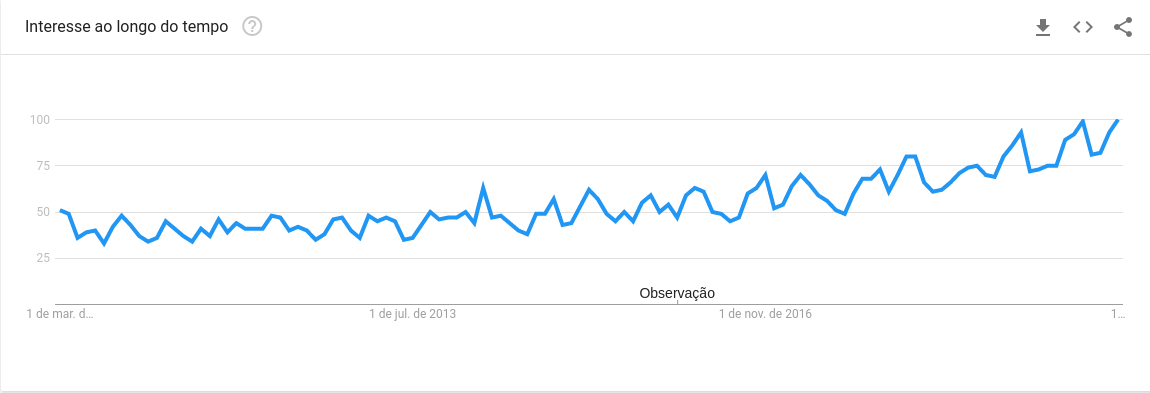
\includegraphics[width=1\linewidth]{imagens/googletrends.png}
	\caption[Número de buscas do termo recommendation system]{Número de buscas do termo "recommendation system" no Google Trends}
	\label{fig:googletrends}
\end{figure}

\nocite{googletrends}
% ----------------------------------------------------------------------

\chapter{\textbf{Objetivos}} % Este comando é utilizado para criar capítulos

\section{Objetivo geral}

Esse trabalho tem como objetivo geral a elaboração de um serviço de recomendação híbrido focado na estruturação dos resultados de algoritmos baseados em filtragem colaborativa e conteúdo.

Além disso, esse trabalho tem como objetivo continuar os estudos apresentados por \citeonline{tcctiago} e \citeonline{tccluisa}, buscando integrar os sistemas desenvolvidos nesses projetos e amplificar os resultados gerados.

Desse modo, o principal objetivo desse trabalho é desenvolver um sistema de recomendação que possua as abordagens colaborativa, baseada em conteúdo e híbrida, possibilitando, com isso, a execução e comparação dos resultados. Espera-se que os resultados obtidos na abordagem híbrida sejam superiores aos da abordagem colaborativa e baseada em conteúdo, quando utilizados de maneira isolada.

\section{Objetivos Específicos}

Como objetivos específicos desse trabalho, considera-se ainda os seguintes itens:
\begin{itemize}
    \item Utilização de técnicas de concorrência nos algoritmos de recomendação desenvolvidos nesse trabalho, buscando desse modo, melhorar a performance do sistema.
    \item Adição de métodos para armazenamento das matrizes de recomendação geradas pelo sistema de forma offline.
    \item Criação de uma aplicação cliente para manipulação e visualização das recomendações, facilitando o processo de acesso aos dados gerados.
    \item Realização de um estudo de caso com recomendação de músicas, avaliando a recomendação híbrida em relação as outras abordagens.
\end{itemize}{}
% ----------------------------------------------------------------------

\chapter{\textbf{Referencial Teórico}}

Nesse capítulo são apresentados os principais conceitos referentes às técnicas aplicadas no desenvolvimento do trabalho, referenciando a literatura e autores utilizados para explicação dos respectivos temas.

\section{Sistemas de Recomendação}

O sistema de recomendação é definido como uma estratégia de tomada de decisão para usuários em ambientes de informação complexos \cite{rashid2002}. Desse modo, a utilização de sistemas de recomendação permite que o usuário consiga lidar com grandes quantidades de informação, provendo recomendações personalizadas e exclusivas do conteúdo analisado \cite{isinkaye2015}.

Para desenvolvimento de um sistema de recomendação, diversos fatores devem ser levados em consideração. De acordo com \citeonline{kimfalk2019}, os seguintes componentes podem ser definidos como a taxonomia \footnote{Taxonomia: no caso citado refere-se a estrutura básica de um sistema de recomendação} de um sistema de recomendação:

\begin{itemize}
	\item \textbf{Domínio}: Refere-se ao tipo de conteúdo recomendado. Com base nesse dado é possível entender, com mais facilidade, o que fazer com as recomendações geradas. Ademais, o conhecimento do domínio possibilita saber qual o custo e impacto que uma recomendação errada poderá gerar ao sistema.
	
	\item \textbf{Objetivo}: Define qual será o foco e estratégia utilizado em cima da recomendação gerada. Principalmente no meio comercial, recomendações com certa tendência a algum produto ou serviço específico podem gerar mais benefícios e lucros para seus criadores, fazendo com que o objetivo da recomendação gere um impacto direto no sistema desenvolvido.
	
	\item \textbf{Contexto}: Refere-se ao ambiente no qual o consumidor utilizará o sistema de recomendação. Esse dado é importante, uma vez que possibilita definir qual será a melhor tecnologia e técnica utilizada no sistema de recomendação. 
	
	\item \textbf{Níveis de personalização}: As recomendações podem apresentar diversos níveis de personalização para seu usuário final, sendo que essas personalizações podem ser divididas em três níveis:
	
	\begin{itemize}
		\item \textit{Não-personalizada}: apresenta as recomendações de forma padronizada para todos os usuários do sistema. Como exemplos típicos dessa abordagem pode-se citar a lista de itens mais populares em um sistema voltado para comércio.
		
		\item \textit{Semi-personalizada ou dividida em segmento}: nesse modelo, o sistema de recomendação procura agrupar os usuários de forma a gerar recomendações voltadas aos interesses de cada grupo.
		
		\item \textit{Personalizada}: nesta abordagem o sistema busca realizar recomendações de acordo com interações passadas do usuário, gerando resultados exclusivos para cada um deles.
	\end{itemize}

	\item \textbf{Quem recomenda}: Em casos específicos, a opinião de especialistas pode apresentar relevância no momento da construção da recomendação, nestes casos, é necessário que esse item seja levado em consideração no desenvolvimento do sistema.
	
	\item \textbf{Privacidade e confiabilidade}: A forma como lidamos com os dados informados e gerados dos usuários é outra questão bastante relevante a ser analisada nos sistemas de recomendação, principalmente em contextos onde informações sigilosas e sensíveis são manipuladas. A confiabilidade refere-se ao quanto o usuário confia nas recomendações ao invés de considerá-las como propagandas ou tentativas de manipulação. O sistema é mais confiável de acordo com que o usuário aceita as recomendações seriamente.
	
	\item \textbf{Interface}: Refere-se aos métodos utilizados para comunicar o usuário ao sistema de recomendação, sendo dividido em \textit{input}: entrada de dados do usuário (de forma explícita ou implícita) e \textit{output}: retorno da recomendação pelo sistema. Em relação ao \textit{output}, pode ser interessante em alguns casos explicar ao usuário como a recomendação é feita. Em um dos estudos de \citeonline{kimfalk2019}, demonstrado na figura \ref{fig:explicabilidade}, é possível analisar a relação entre o nível de acurácia da recomendação e a facilidade de explicação ao usuário de como a mesma foi feita:
	
	\begin{figure}[H]
		\centering
		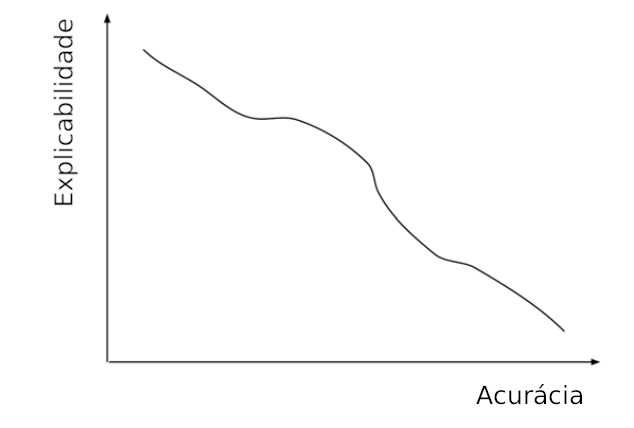
\includegraphics[width=0.7\linewidth]{imagens/explicabilidade}
		\caption[Explicabildade vs. qualidade da recomendação]{Explicabildade vs. qualidade da recomendação}
		\label{fig:explicabilidade}
	\end{figure}
	 
	\item \textbf{Algoritmos}: Existem diversos algoritmos que podem ser utilizados na construção de um sistema de recomendação. Esses algoritmos costumam ser divididos em dois grupos: \textbf{filtragem colaborativa} e \textbf{baseada em conteúdo}, sendo que a escolha do tipo de algoritmo dependerá do tipo de dado utilizado para construção das recomendações. Uma abordagem \textbf{híbrida} também pode ser utilizada, mesclando técnicas dos dois grupos apresentados.
\end{itemize}

\subsection{Filtragem Colaborativa}

O algoritmos de filtragem colaborativa têm como objetivo explorar informações a partir das experiências dos usuários para recomendação de itens \cite{sedhain2015}. Para isso, esses algoritmos utilizam técnicas como a fatoração matricial como apresentado por \citeonline{koren2009}, \citeonline{lee2013} e modelos de vizinhança como definido por \citeonline{sarwar2001}, de forma a recomendar itens parecidos para usuários com certo nível de proximidade \cite{kimfalk2019}.

Um dos problemas ao utilizar-se dessa abordagem é a dependência existente entre a recomendação e os dados dos demais usuários, fazendo com que as recomendações geradas na fase inicial desses sistemas possam apresentar desvios nos resultados gerados \citeonline{wei2017collaborative} e \cite{choi2010content}.

Esse modelo de recomendação é bastante conhecido, sendo um dos mais utilizados nos sistemas de recomendação \cite{alyari2018}.

\subsection{Filtragem baseada em Conteúdo}

A filtragem baseada em conteúdo, como definido por \citeonline{kimfalk2019}, é um modelo de algoritmo que utiliza de metadados para gerar as recomendações dos itens. Nesses sistemas, é buscada a criação de um perfil para os usuários baseado nos itens do sistema, de forma com que seja possível comparar esse perfil aos itens para geração das recomendações.

Como principal problema dessa abordagem de recomendação têm-se o momento em que um novo usuário acaba de ser criado, uma vez que o sistema não consegue inferir quais são os tópicos (assuntos ou tags) de maior relevância para esse usuário, reduzindo a taxa de acertos nas recomendações iniciais \cite{inbook}.

\subsection{Recomendação Híbrida}

Abordagens de recomendação colaborativas e baseadas em conteúdo apresentam pontos positivos e negativos \cite{kimfalk2019}. A recomendação baseada em conteúdo apresenta alguns problemas associados a análise limitada das informações, superespecialização e escassez de dados como demonstrado por \citeonline{adomavicius2005}, enquanto que a abordagem colaborativa apresenta problemas relacionados principalmente a escalabilidade e manipulação de bases com baixo volume de dados \cite{isinkaye2015}.

Com intuito de melhorar a qualidade da recomendação e como forma de mitigar alguns dos problemas identificados, foi proposto o modelo de filtragem híbrida, que busca a partir da combinação das técnicas de filtragem, aumentar o desempenho e precisão dos sistemas de recomendação \cite{goksedef2010}. Com essa abordagem, busca-se aproveitar os pontos fortes vistos em cada uma das abordagens, como também, nivelar suas fraquezas \cite{al2008}. 

Diversas estratégias podem ser utilizadas na recomendação híbrida, onde as principais, levando em conta a forma como os componentes serão combinados para gerar as recomendações, são as seguintes  \cite{barbosa2014}:

\begin{itemize}
    \item \textbf{Ponderada:} nesse modelo de abordagem, as filtragens colaborativa e baseada em conteúdo são aplicadas de forma separada, sendo que, após a geração das recomendações, é realizado um processo de combinação linear, utilizando os resultados gerados. Em alguns casos, pode ser necessário a realização de uma normalização entre os dados, caso os mesmos estejam em escalas diferentes.
    
    \item \textbf{Mista:} nesse modelo as recomendações geradas são mescladas para geração do resultado final. Desde modo, o resultado apresentado ao usuário será uma lista com os dados gerados na recomendação colaborativa e baseada em conteúdo.
    
    \item \textbf{Combinação sequencial:} nesse modelo temos a criação de um perfil do usuário, em um primeiro momento, a partir da recomendação baseada em conteúdo. A partir dos perfis criados, é realizada a recomendação colaborativa que gerará os resultados finais dessa abordagem.
    
    \item \textbf{Comutação:} para essa abordagem, é necessário a utilização de algum critério para avaliação, que pode ser definido de acordo com a natureza do sistema. Esse critério é utilizado para comutar ou chavear os resultados obtidos na recomendação colaborativa e baseada em conteúdo, gerando o resultado final. Outra abordagem válida é a comutação de uma técnica nos pontos de desvantagens da outra.
\end{itemize}

Vale ressaltar, que a escolha da metodologia aplicada variará de acordo com a natureza do problema em questão.

\subsection{Matriz de Recomendação offline}

O processo de recomendação nos sistemas, pode ocorrer de três maneiras diferentes: recomendação online, offline e a combinação das duas formas anteriores. De acordo com \citeonline{gunawardana2009survey} a recomendação offline deve ser utilizada para identificação dos itens mais promissores, para que os mesmos possam ser submetidos ao processo de recomendação online.

Para realização dessa abordagem, é necessário o armazenamento do conjunto de dados utilizados na recomendação, sendo que, segundo \citeonline{gunawardana2009survey}, os dados devem se assemelhar o máximo possível com os dados usados na abordagem online. Utilizando essa técnica de recomendação têm-se uma melhoria na performance do processo, uma vez que se diminui o tempo da tarefa de recomendação no ponto de vista dos utilizadores \cite{moreira2019sistema}.

\section{Programação Concorrente}

Em diversas aplicações, múltiplas atividades podem ocorrer ao mesmo tempo. Desse modo, é possível decompor uma aplicação em múltiplas threads(linhas de execução) sequenciais que executem de forma paralela \cite{tanenbaum2015modern}. Pode-se analisar, na figura \ref{fig:threads}, um exemplo de sistema de edição de texto utilizando três threads simultaneamente. Nesse exemplo simplificado, é possível observar as seguintes funções para cada thread:

\begin{itemize}
    \item \textbf{Thread 1:} Receber os dados informados pelo teclado;
    \item \textbf{Thread 2:} Exibir o texto no editor (tela da aplicação);
    \item \textbf{Thread 3:} Salvar os dados informados no disco (função de auto-salvamento).
\end{itemize}

\begin{figure}[H]
		\centering
		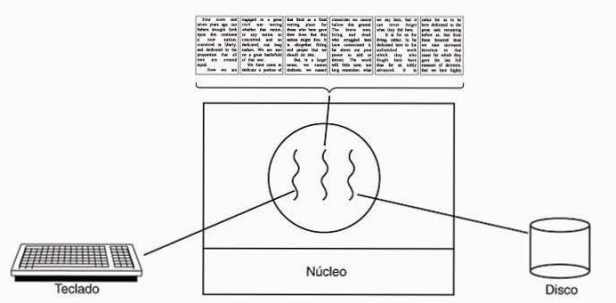
\includegraphics[width=0.8\linewidth]{imagens/threads.png}
		\caption[Uso de threads em um sistema de edição de texto]{Uso de threads em um sistema de edição de texto \cite{tanenbaum2007distributed}}
		\label{fig:threads}
	\end{figure}

O uso de threads possibilita o aumento de desempenho das aplicações que possuem muitos processos de E/S, devido a sobreposição possível entre as linhas de execução \cite{tanenbaum2015modern}.

\textbf{Diferença entre threads e processos}

Segundo \citeonline{tanenbaum2015modern}, um processo pode ser definido como um programa em execução que possui valores de um contador de programa (que define até onde o processo já foi executado), registradores e variáveis. Desse modo, os processos podem ser considerados programas independentes, sendo executados de acordo com o escalonamento definido pelo sistema operacional. Na figura \ref{fig:processos}, é possível visualizar uma exemplo de execução de quatro processos em um sistema:

\begin{figure}[H]
		\centering
		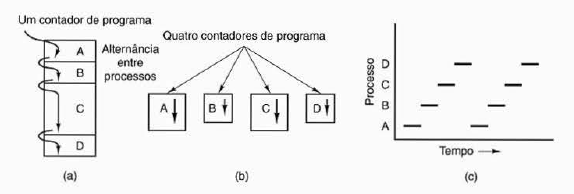
\includegraphics[width=1\linewidth]{imagens/processos.png}
		\caption[Exemplo de execução de quatro processos]{Exemplo de execução de quatro processos \cite{tanenbaum2015modern}}
		\label{fig:processos}
	\end{figure}

Enquanto isso, uma thread pode ser considerada uma linha de execução que compartilha recursos e o espaço de endereçamento da memória, executando de forma quase paralela \cite{tanenbaum2015modern}. A principal razão para seu uso é em aplicações onde ocorram diversas operações ao mesmo tempo, fazendo com que o modelo de programação seja facilitado a partir do uso de threads \cite{tanenbaum2015modern}.

Como definido por \citeonline{tanenbaum2015modern}, existe três argumentos para utilização de threads em um sistema:

\begin{itemize}
    \item \textbf{Compartilhamento de recursos:} capacidade de entidades paralelas compartilharem um mesmo espaço de endereçamento de memória e dados.
    \item \textbf{Velocidade:} as threads são mais fáceis e rápidas de serem destruídas que os processos, uma vez que não possuem quaisquer recursos vinculados a elas. Além disso, em muitos sistemas, a criação de threads é cerca de até cem vezes mais rápida que a criação de um processo. Esse fator é bastante útil em aplicações que o número de threads se altera de forma rápida e dinâmica.
    \item \textbf{Desempenho:} a utilização de threads em processos de E/S (entrada e saída) pode resultar em melhoria de performance da aplicação, já que as threads possibilitam a sobreposição dessas tarefas. 
\end{itemize}

\subsection{Ciclos de Vida e estados da thread}

Durante a execução de um programa concorrente, uma thread pode apresentar vários estados, como definido por \citeonline{deitel2016} e apresentado na figura \ref{fig:ciclovidathread}:

\begin{figure}[H]
	\centering
	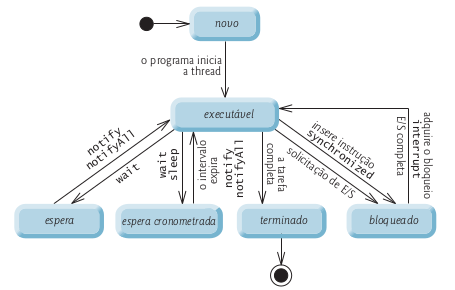
\includegraphics[width=0.8\linewidth]{imagens/cicloVidaThread}
	\caption[Estado e ciclo de vida da thread]{Diagrama de estado e ciclo de vida da thread \cite{deitel2016}}
	\label{fig:ciclovidathread}
\end{figure}

Muitos desses estados são abstraídos pelas linguagens de programação de alto nível, simplificando o processo de desenvolvimento. Porém, para aplicações com rotinas mais avançadas, o conhecimento desses estados e o ciclo de vida das threads torna-se trivial, pois permite ao programador um maior nível de controle sobre o software \cite{deitel2016}. Dessa forma, baseando na obra de \citeonline{deitel2016}, é apresentado abaixo os ciclos e estados que uma thread pode obter durante a execução de um software concorrente.

\textbf{Estado novo e executável}

Uma nova thread tem seu ciclo de vida iniciado com o estado \textbf{novo}. Esse estado é mantido até que o programa inicie a thread, mudando seu estado para \textbf{executável}, que é mantido enquanto essa thread encontra-se em execução.

\textbf{Estado de espera}

Uma thread em estado \textit{executável} transita para o estado de \textbf{espera} quando é necessário aguardar que outra thread realize alguma tarefa. A thread em \textit{espera} volta ao estado \textit{executável} quando é notificada por outra thread que continue sua execução.

\textbf{Estado de espera sincronizada}

Uma thread que está no estado \textit{executável} pode entrar no estado de \textbf{espera sincronizada} por um determinado período de tempo, voltando para o estado \textit{executável} após término desse período ou de um evento que ela esteja aguardando. Threads nesse estado não poderão utilizar o processador, mesmo que ele esteja disponível.

Em determinadas situações, uma thread \textit{executável} pode transitar para o estado de \textit{espera sincronizada} ao fornecer um intervalo de espera opcional, procurando, dessa forma, esperar a realização de alguma tarefa realizada por outra thread.

\textbf{Estado bloqueado}

Uma thread \textit{executável} pode entrar no estado \textbf{bloqueado} ao tentar realizar uma tarefa que não pode ser concluída imediatamente, fazendo com que a thread tenha que esperar até que a tarefa bloqueante seja concluída. Threads nesse estado não poderão acessar o processador, mesmo que ele esteja disponível.

\textbf{Estado terminado}

Ocorre quando uma thread \textit{executável} conclui com sucesso sua tarefa, o que faz com que a mesma mude para o estado \textbf{terminado} (às vezes chamado de estado \textbf{morto}). Esse estado também pode ocorrer caso a thread seja terminada por outro motivo, como razão de um erro, por exemplo. 

\subsection{Sincronização de threads}

Em momentos que várias threads compartilham um objeto que é modificado por uma ou mais delas, podem ocorrer resultados indeterminados caso a manipulação e acesso a esse objeto ocorra de forma incorreta. Neste tipo de caso, o comportamento do programa torna-se não confiável, uma vez que os resultados produzidos dependeram da forma que o acesso as threads é manipulado pelo sistema operacional \cite{deitel2016}. 

Esse problema pode ser resolvido fornecendo acesso a somente uma thread, por vez, ao objeto compartilhado, fazendo com que as outras threads não tenham acesso ao objeto durante esse período, aplicando dessa forma, o conceito de \textbf{exclusão mútua}. Quando a thread com acesso exclusivo ao objeto termina sua tarefa, outras threads em espera poderão utilizar o recurso compartilhado, fazendo com que o acesso aos dados seja coordenado e organizado a partir da \textbf{sincronização das threads} envolvidas \cite{tanenbaum2015modern}.

\section{Sistemas Distribuídos}

Um sistema distribuído, como definido por \citeonline{tanenbaum2007distributed} pode ser descrito como um conjunto de computadores autônomos não obrigatoriamente equivalentes, interligados entre si, sendo compreendidos e apresentados ao usuário como um sistema único.

A comunicação e coordenação das ações entre esses componentes opera-se a partir do envio de mensagens, sendo que a transmissão pode através de redes como a internet ou bluetooth, por exemplo \cite{coulouris2013sistemas}. 

Segundo \citeonline{coulouris2013sistemas}, ao se utilizar a arquitetura de sistemas distribuídos, têm-se como consequência os seguintes pontos:

\begin{itemize}
    \item \textbf{Concorrência:} em uma rede de computadores, o uso da concorrência é de suma importância, uma vez que possibilita a execução de diversas atividades de forma simultânea, no ponto de vista do usuário. Sua utilização permite a distribuição de recursos nos sistemas distribuídos, o que faz esse tópico ser de extrema importância em sistemas que necessitem de boa performance para funcionamento.
    
    \item \textbf{Inexistência de relógio global:} em um sistema que trabalha e coordena suas atividades através da troca de mensagens, torna-se necessário o estabelecimento de uma noção de tempo compartilhada entre seus componentes. Um problema relacionado a esse fator é o limite de precisão existente ao sincronizar esses componentes, o que acaba sendo uma consequência direta do uso da comunicação através da troca de mensagens.
    
    \item \textbf{Falhas independentes:} em qualquer sistema de computadores falhas poderão ocorrer, o que faz com que ao se projetar um sistema seja necessário analisar e prever as consequências de possíveis falhas. Em um sistema distribuído essas falhas podem ocorrer tanto em nível de hardware e software como ainda na rede, impossibilitando ou dificultando a comunicação entre os componentes.
\end{itemize}

Vários benefícios dos sistemas distribuídos podem ser citados em relação aos sistemas centralizados, como redundância, escalabilidade, tolerância a falhas e economia de recursos \cite{puder2011distributed}.

\subsection{Web Services}

Os \textit{web services} podem ser classificados como softwares fornecidos por uma rede (como a internet, por exemplo). São entidades executáveis que funcionam de maneira modular e independente, sendo acessadas e publicadas em uma rede \cite{falter2009system}.
 
 \textbf{Modelo REST (\textit{Representational State Transfer})}
 
 De acordo com \citeonline{falter2009system}, os web services são serviços portáveis entre as diversas plataformas de computação, isso ocorre devido a adoção de padrões e metodologias amplamente aceitas na comunidade de desenvolvimento desses sistemas. Como exemplo de padrão para arquitetura dos sistemas na web pode-se citar o modelo REST(\textit{Representational State Transfer}, definido por \citeonline{fielding2000architectural}, um dos grandes colaboradores do protocolo HTTP, que acabou por defender o uso do modelo no protocolo da internet.

O modelo REST apresenta algumas atribuições básicas, criadas por \cite{fielding2000architectural}. Elas podem ser definidas como:

\begin{itemize}
		\item Os sistemas devem seguir a \textbf{arquitetura cliente-servidor}, permitindo desse modo a independência e separação das responsabilidades entre os sistemas, além de favorecer a escalabilidade desses sistemas.
		
		\item A comunicação entre os sistema deve ocorrer \textbf{sem estado (\textit{stateless})}, sendo de responsabilidade da aplicação cliente manter, caso necessário, a sessão do usuário. Essa ideia possibilita uma maior escalabilidade do sistema, além de se apoiar em outros princípios como visibilidade e confiabilidade dos dados.
		
		\item Como forma de se obter um melhor desempenho na comunicação, pode-se ser utilizado a \textbf{estratégia de cache nas requisições}, evitando dessa forma, processamento desnecessário uma vez que o cache mantém dados já requisitados armazenados, fazendo com que a aplicação não tenha necessidade de buscá-los novamente caso a mesma consulta seja realizada.
		
		\item Os sistemas REST devem possuir uma ênfase em construir uma \textbf{interface uniforme entre os componentes}. O que acaba resultando em uma interface mais visível e simples entre as interações e comunicação.
		
		\item A criação dos sistemas REST devem ser pensadas em uma \textbf{estrutura de camadas}, onde cada componente deve saber apenas interagir com suas camadas vizinhas. Com isso os componentes podem usufruir de uma estrutura menos complexa além de permitir um melhor encapsulamento e separação das responsabilidades.
		
		\item Os sistemas podem possuir, de maneira opcional, \textit{applets} e \textit{scripts} que possam ser disponibilizados para os clientes, facilitando a implementação dos sistemas REST. Essa estratégia pode ser definida como \textbf{entrega de código sob demanda}.
	\end{itemize}

A realização da comunicação nesse modelo de arquitetura é realizada a partir do protocolo HTTP, onde os verbos do HTTP definem qual tipo de operação será realizada com o recurso requerido na requisição.

Na tabela , pode-se analisar a correspondência entre os métodos HTTP e as operações realizadas nas requisições de acordo com a \citeonline{rfc7231} e \citeonline{rfc7231}:

\begin{table}[H]
\begin{tabular}{c|l}
\textbf{Método HTTP} & \multicolumn{1}{c}{\textbf{Operação}}                        \\ \hline
GET                  & Solicita recurso (leitura)                                   \\
HEAD                 & Solicita resposta igual o GET, porém sem corpo na resposta   \\
POST                 & Cria um recurso                                              \\
PUT                  & Altera um recurso                                            \\
DELETE               & Remove um recurso                                            \\
CONNECT              & Estabelece um túnel de conexão ao servidor                   \\
OPTIONS              & Solicita os métodos e opções disponíveis no servidor         \\
TRACE                & Executa um teste de chamada loop-back ao servidor de destino \\
PATCH                & Realiza alterações parciais em um recurso                  \label{table:metodoHttp} 
\end{tabular}
\end{table}

O modelo de arquitetura definido por \citeonline{fielding2000architectural} mostra-se uma excelente opção aos tradicionais \textit{web services} SOAP \footnote{Protocolo para troca de mensagens em sistemas distribuídos. Baseia-se na estrutura de XML para representação dados, sendo comumente combinado com protocolos como o HTTP \cite{box2000simple}} disponíveis, principalmente em relação ao desempenho que se beneficia de menores tempos de respostas e trafégos de dados na arquitetura REST como apresentado por \citeonline{saad2010performance} e \citeonline{dudhe2014performance}.
	
Na figura \ref{fig:rest} é possível observar uma representação básica de um \textit{web service} utilizando a arquitetura REST. Neste exemplo, uma aplicação cliente realiza requisições HTTP (\textit{HTTP Request}) ao servidor que responde com outra requisição (\textit{HTTP Response}), utilizando algum formato para representação de estado do recurso solicitado (XML, JSON, HTML, TEXT).

\begin{figure}[H]
	\centering
	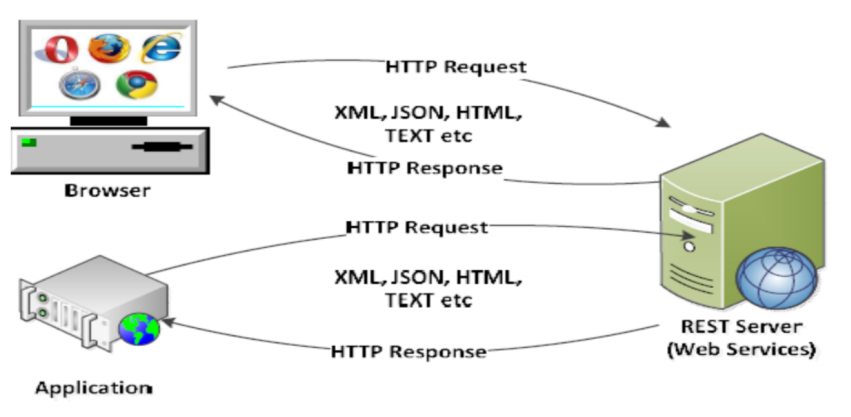
\includegraphics[width=0.9\linewidth]{imagens/rest.png}
	\caption[Exemplo de arquitetura REST]{Exemplo de arquitetura REST \cite{thu2015developing}}
	\label{fig:rest}
\end{figure}

\textbf{RESTful}

Como forma de mensurar a qualidade dos sistemas REST, \citeonline{richardson2008justice} definiu um modelo que possibilita a avaliação do nível de maturidade da arquitetura implementada. Esse modelo é dividido em quatro níveis, sendo que o autor define o último nível como a "glória dos sistemas REST". A organização desses níveis pode ser vista na figura \ref{fig:restNiveis}:

\begin{figure}[H]
	\centering
	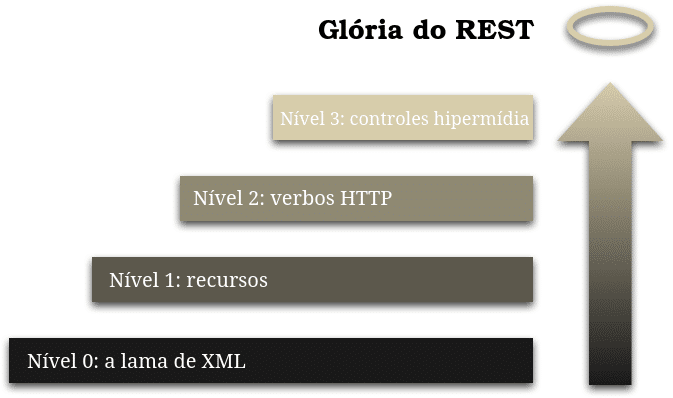
\includegraphics[width=0.7\linewidth]{imagens/restNiveis.png}
	\caption[Níveis da arquitetura REST]{Níveis da arquitetura REST \cite{fowler2010richardson} (adaptado)}
	\label{fig:restNiveis}
\end{figure}

Segundo \citeonline{richardson2008justice} os níveis da arquitetura podem ser definidos da seguinte forma:

\begin{itemize}
    \item \textbf{Nível 0:} Como ponto de partida do modelo, têm-se a utilização do protocolo HTTP para transporte das solicitações, sem utilização de qualquer mecanismos da web. Neste modo, o uso do HTTP apresenta-se normalmente a partir de um mecanismo de encapsulamento, onde é feita uma requisição para determinado endereço que irá realizar a chamada de algum método do sistema, como apresentado na figura \ref{fig:nivel0}. Neste nível, não existe preocupação em relação aos status e retorno das requisições realizadas.
    
    \begin{figure}[H]
    	\centering
    	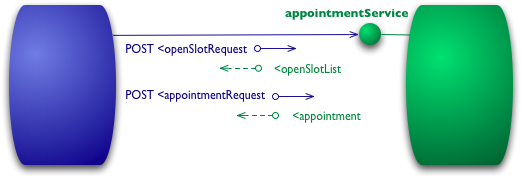
\includegraphics[width=0.7\linewidth]{imagens/level0.png}
    	\caption[Nível 0 no modelo de maturidade]{Nível 0 no modelo de maturidade \cite{fowler2010richardson}}
	    \label{fig:nivel0}
    \end{figure}
    
    \item \textbf{Nível 1:} Para atingir esse nível de maturidade, é necessário a introdução de recursos no sistema. Então, levando em conta a figura \ref{fig:nivel0}, ao invés da chamada a um método do sistema, será realizada a requisição de um recurso, como apresentado na figura \ref{fig:nivel1}:
    
    \begin{figure}[H]
    	\centering
    	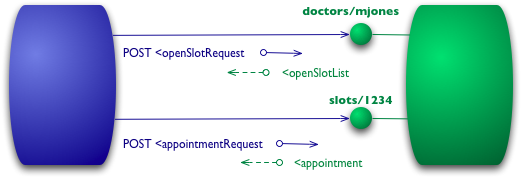
\includegraphics[width=0.7\linewidth]{imagens/level1.png}
    	\caption[Nível 1 no modelo de maturidade]{Nível 1 no modelo de maturidade \cite{fowler2010richardson}}
	    \label{fig:nivel1}
    \end{figure}
    
    \item \textbf{Nível 2:} Neste nível, têm-se a preocupação da correta utilização dos verbos HTTP e seus respectivos status, o que acaba tornando as operações mais semânticas e legíveis para seus utilizadores. Na figura \ref{fig:nivel2}, podemos ver as alterações em relação ao nível 1:
    
    \begin{figure}[H]
    	\centering
    	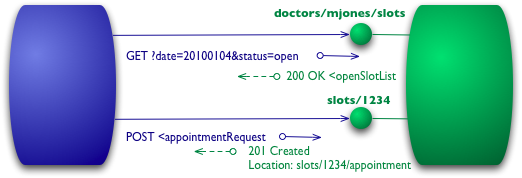
\includegraphics[width=0.7\linewidth]{imagens/level2.png}
    	\caption[Nível 2 no modelo de maturidade]{Nível 2 no modelo de maturidade \cite{fowler2010richardson}}
	    \label{fig:nivel2}
    \end{figure}
    
    \item \textbf{Nível 3:} No nível final de maturidade, é vista a introdução do conceito de HATEOAS (\textit{Hypertext As The Engine Of Application State}). Esse recurso possibilita uma visão dos relacionamentos e das ações possíveis a partir de determinado recurso no sistema. Para realização dessa técnica, são utilizados \textit{hyperlinks} que serão enviados juntamente com a resposta do servidor, explicitando os recursos e ações vinculados ao recurso solicitado. Na figura \ref{fig:nivel3}, temos uma visão desse nível:
    
    \begin{figure}[H]
    	\centering
    	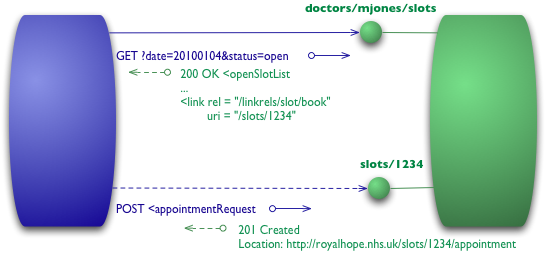
\includegraphics[width=0.7\linewidth]{imagens/level3.png}
    	\caption[Nível 3 no modelo de maturidade]{Nível 3 no modelo de maturidade \cite{fowler2010richardson}}
	    \label{fig:nivel3}
    \end{figure}
\end{itemize}

A utilização do modelo RESTful permite a criação de aplicações distribuídas escaláveis, além de adicionar poderosas descrições e interoperabilidade entre os dados semânticos fornecidos pelo sistema \cite{restfulPerformance}.
%%% ====================================================================
%%% Início da parte textual do documento.


%%% Configuração do espaçamento entre títulos e texto
\setlength{\afterchapskip}{1.5cm minus \baselineskip}


\chapter{Metodologia}
\label{cha:metodologia}

\section{Arquitetura utilizada}

\subsection{Componentes}

Para elaboração do sistema proposto, foi utilizado uma arquitetura baseada em sistemas distribuídos, que a partir do protocolo HTTP comunica-se entre seus componentes. Esses componentes podem ser vistos na figura \ref{fig:arquitetura}:

\begin{figure}[H]
	\centering
	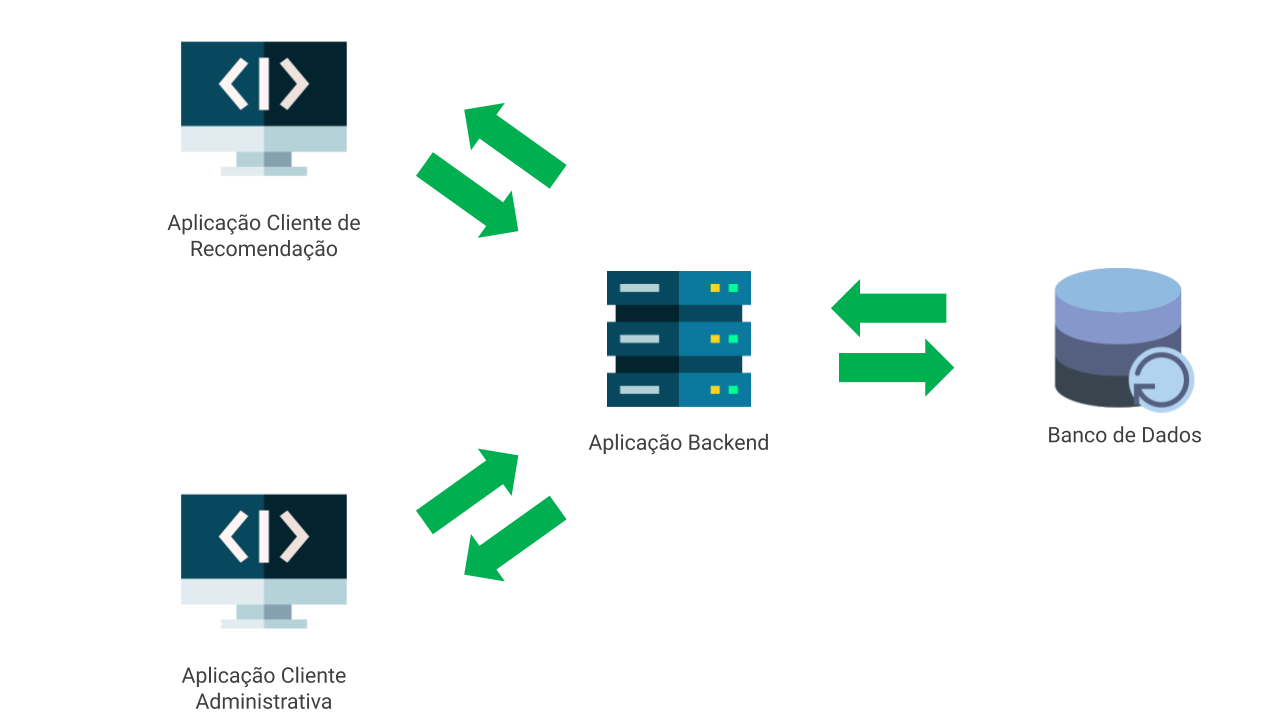
\includegraphics[width=0.7\linewidth]{imagens/arquitetura.png}
	\caption[Arquitetura do sistema]{Arquitetura do sistema (AUTOR, 2020)}
    \label{fig:arquitetura}
\end{figure}

Cada um dos componentes definidos apresenta uma respectiva função no sistema, que pode ser observada abaixo:

\begin{itemize}
    \item \textbf{Backend:} responsável pelo processamento e gerenciamento das recomendações e de todos os recursos existentes no sistema.
    
    \item \textbf{Cliente Administrativo:} aplicação gráfica para acesso e manipulação dos recursos pelo administrador do sistema. Nessa aplicação o administrador poderá manipular os recursos relacionados aos seus casos de uso além de poder emitir diversas listagens e relatórios para avaliação dos resultados gerados pelo sistema.
    
    \item \textbf{Cliente de Recomendação:} aplicação gráfica para acesso e manipulação dos recursos pelos avaliadores do sistema.
\end{itemize}

\subsection{Tecnologias}

As seguintes tecnologias foram utilizadas para elaboração do sistema:

\begin{itemize}
    \item \textbf{Java 14:} linguagem escolhida para desenvolvimento do backend devido a facilidade de implementação de concorrência e por ter sido utilizada na elaboração dos algoritmos usados como base para elaboração do sistema proposto.
    
    \item \textbf{Spring Boot 2.2.6:} framework utilizado para desenvolvimento da arquitetura web do backend. Possui diversas bibliotecas e implementações que facilitam o desenvolvimento de sistemas robustos e seguros.
    
    \item \textbf{PostgreSQL:} sistema de banco de dados que utiliza a especificação SQL em seu funcionamento.
    
    \item \textbf{H2:} sistema de banco de dados em memória utilizado para testes da aplicação.
    
    \item \textbf{VueJS:} Framework web baseado em Javascript, possui diversas ferramentas e recursos que facilitam o processo de desenvolvimento. 
    
    \item \textbf{Quasar Framework:} biblioteca baseada no VueJS que dispõe inúmeros componentes e estruturas para desenvolvimento de sistemas web com alta performance. Utilizado para desenvolvimento dos clientes frontend do sistema.
    
    \item \textbf{JWT:} especificação para transferência segura de dados a partir de requisições HTTP, definida na RFC 7519 \cite{ietftools}. Segundo \citeonline{jones2015json}, o JWT apresenta-se como uma alternativa concreta para transmissão de informações confidenciais em sistemas stateless.
\end{itemize}


\subsection{Ferramentas}

No processo de desenvolvimento do sistema proposto, foram utilizadas as seguintes ferramentas:

\begin{itemize}
    \item \textbf{IntelliJ IDEA Community:} IDE utilizada para desenvolvimento do backend da aplicação e gerenciamento de suas dependências.

    \item \textbf{PhpStorm:} IDE utilizada para desenvolvimento dos clientes frontend e gerenciamento de suas dependências.

    \item \textbf{Git e Github:} Ferramentas utilizadas respectivamente no versionamento e na criação e publicação dos repositórios na internet.

    \item \textbf{pgAdmin4:} ferramenta gráfica para manipulação e gerenciamento do banco de dados PostgreSQL.
    
    \item \textbf{Postman:} ferramenta utilizada para realização de requisições HTTP para o sistema e na geração de documentação para a API.

    \item \textbf{Adobe XD:} ferramenta utilizada para criação dos protótipos e wireframes dos clientes frontend do sistema.

    \item \textbf{Docker e Docker Compose:} ferramentas baseadas em containers e utilizadas na criação do banco de dados PostgreSQL e na ferramenta pgAdmin4, possibilitando uma melhor interoperabilidade entre diversos sistemas operacionais.
    
    \item \textbf{UML (Unified Modeling Language):} ferramenta para modelagem do sistema, que segundo \citeonline{booch2006uml}, pode ser definida como uma linguagem gráfica utilizada para visualização, construção, especificação e documentação de artefatos em sistemas de software complexos.
    
    \item \textbf{Astah Community:} ferramenta utilizada na criação dos diagramas UML para documentação do backend do sistema.
    
    \item \textbf{Git Flow:} ferramenta utilizada para organização e fluxo dos versionamentos de código. O modelo apresentado pelo Git Flow permite aos desenvolvedores um maior controle das ramificações \textit{(branch)} e fluxos de trabalho criados no Git, organizando e separando controle de recursos, hotfixes \footnote{Mudanças de código pontuais, normalmente utilizadas para correções de bugs \cite{chopra2014automated}} e versões em softwares de maior escala \cite{kreeftmeijer2015using}.
\end{itemize}

\section{Algoritmo}

Para desenvolvimento dos algoritmos de filtragem colaborativa e baseada em conteúdo, foram usados como base, respectivamente, os trabalhos de \citeonline{tcctiago} e \citeonline{tccluisa}. A recomendação híbrida combina os dois métodos de recomendações (colaborativa e baseada em conteúdo) e gera seus resultados de acordo com a abordagem definida para execução do algoritmo. Todos os cálculos podem serem vistos detalhadamente na seção de Anexos desse trabalho.

\subsection{Distância euclidiana}

O cálculo da distância euclidiana prove a medição da distância entre dois pontos, permitindo desse modo, sua utilização para definição da similaridade entre os objetos de um sistema de recomendação. A fórmula da distância euclidiana pode ser visualizada abaixo:

\begin{equation*}
    DE\left( x,y\right)   = \sqrt {\sum _{i}^{p}  \left( x_{i}-y_{i}\right)^2 }
    \label{eq:euclidiana}
\end{equation*}

\subsection{Recomendação colaborativa}

Para exemplificação do algoritmo de filtragem colaborativa, será utilizado o exemplo apresentado na figura \ref{fig:algoritmocolaborativo}:

\begin{figure}[H]
	\centering
	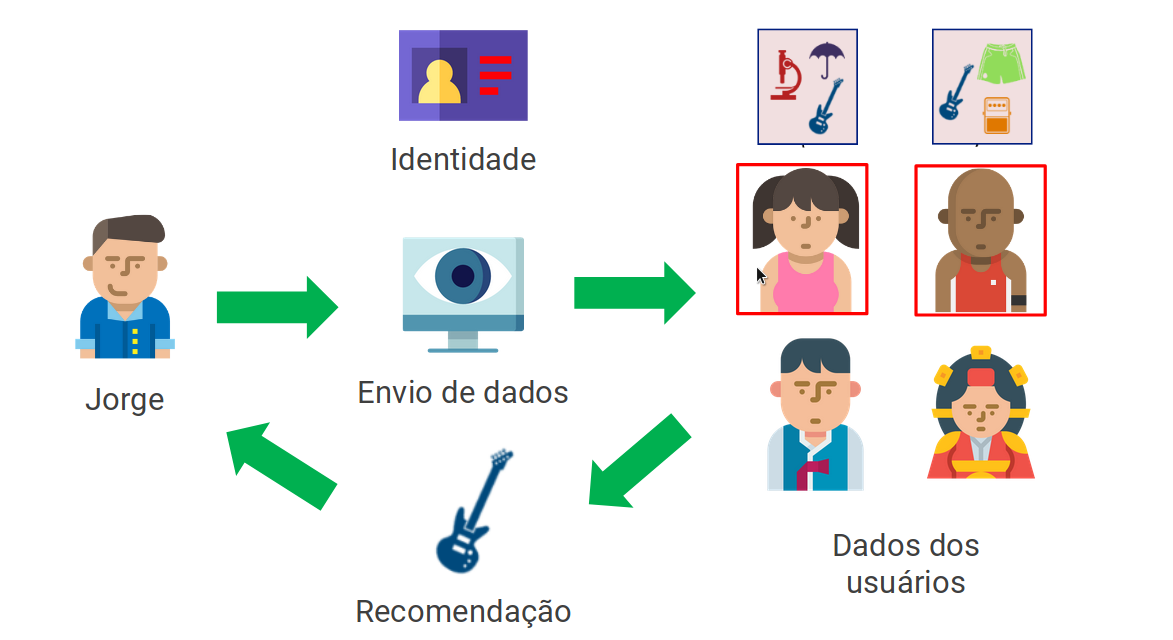
\includegraphics[width=0.7\linewidth]{imagens/colaborativa.png}
	\caption[Exemplo de filtragem colaborativa]{Exemplo de filtragem colaborativa, adaptado de \cite{araujo2011apprecommender}}
    \label{fig:algoritmocolaborativo}
\end{figure}

No seguinte exemplo, têm-se um usuário (definido como Jorge) que está acessando um site de vendas que possui um sistema de recomendação baseado em conteúdo. Durante o acesso de Jorge ao site, o sistema realiza uma coleta e análise de seus dados de navegação, procurando traçar o seu perfil de usuário (representado como a identidade na figura \ref{fig:algoritmocolaborativo}). Esse perfil é utilizado para quantificação e análise da avaliação do Jorge acerca dos produtos do site.

A partir da comparação do perfil do Jorge com o de outros usuários, é possível definir um vínculo de similaridade entre os perfis de ambos. Com isso, é possível identificar quais os usuários com os gostos mais parecidos com o Jorge, esses usuários são identificados como vizinhos.

Com a análise dos perfis dos vizinhos, torna-se possível identificar quais seriam os prováveis itens que poderiam ser recomendados ao Jorge, levando em conta que provavelmente os itens comprados pelos vizinhos atendem ao gosto do Jorge. 

\subsection{Recomendação baseada em conteúdo}

Para exemplificação do algoritmo de filtragem baseada em conteúdo, será utilizado o exemplo apresentado na figura \ref{fig:algoritmoconteudo}:

\begin{figure}[H]
	\centering
	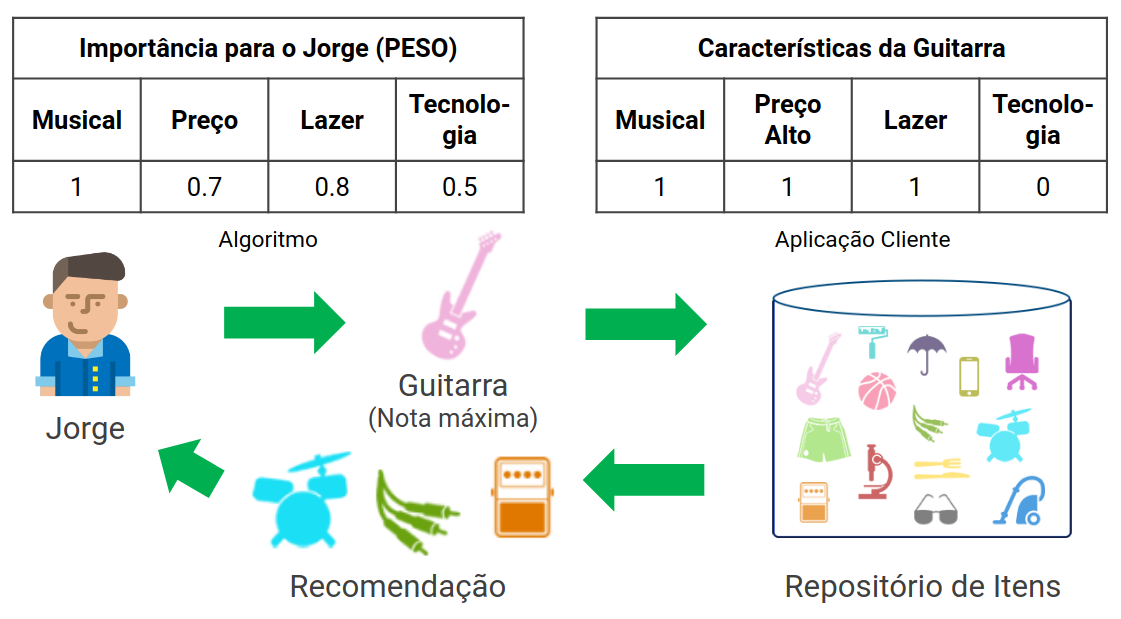
\includegraphics[width=0.7\linewidth]{imagens/baseadoconteudo.png}
	\caption[Exemplo de filtragem baseada em conteúdo]{Exemplo de filtragem baseada em conteúdo, adaptado de \cite{araujo2011apprecommender}}
    \label{fig:algoritmoconteudo}
\end{figure}

No seguinte exemplo, temos o mesmo caso apresentado no algoritmo de filtragem colaborativa, contudo utilizando a abordagem de recomendação baseada em conteúdo.

No caso apresentado, o usuário Jorge realiza a compra de uma guitarra em um site de compras que está utilizando a abordagem baseada em conteúdo para recomendação de produtos. Nesse modelo de produto, foram definidos algumas tags que possuem uma nota que define o quanto o produto atende a característica definida na tag em questão (tabela de características da guitarra).

A partir dessa tabela de característica, somada a dos outros produtos que Jorge possa ter comprado ou avaliado, é possível gerar uma tabela de importância das tags para o Jorge, que definirá quais os atributos que ele considera mais importantes na compra de um produto.

Com essa tabela gerada, é possível utilizá-la para multiplicação e geração dos pesos que Jorge possivelmente dará aos produtos ainda não avaliados. Logo, torna-se possível recomendar os itens que possuam as melhores notas.

\subsection{Recomendação Híbrida}

Na recomendação híbrida é utilizado uma combinação das abordagens colaborativa e baseada em conteúdo conforme a figura \ref{fig:algoritmohibrido}:

\begin{figure}[H]
	\centering
	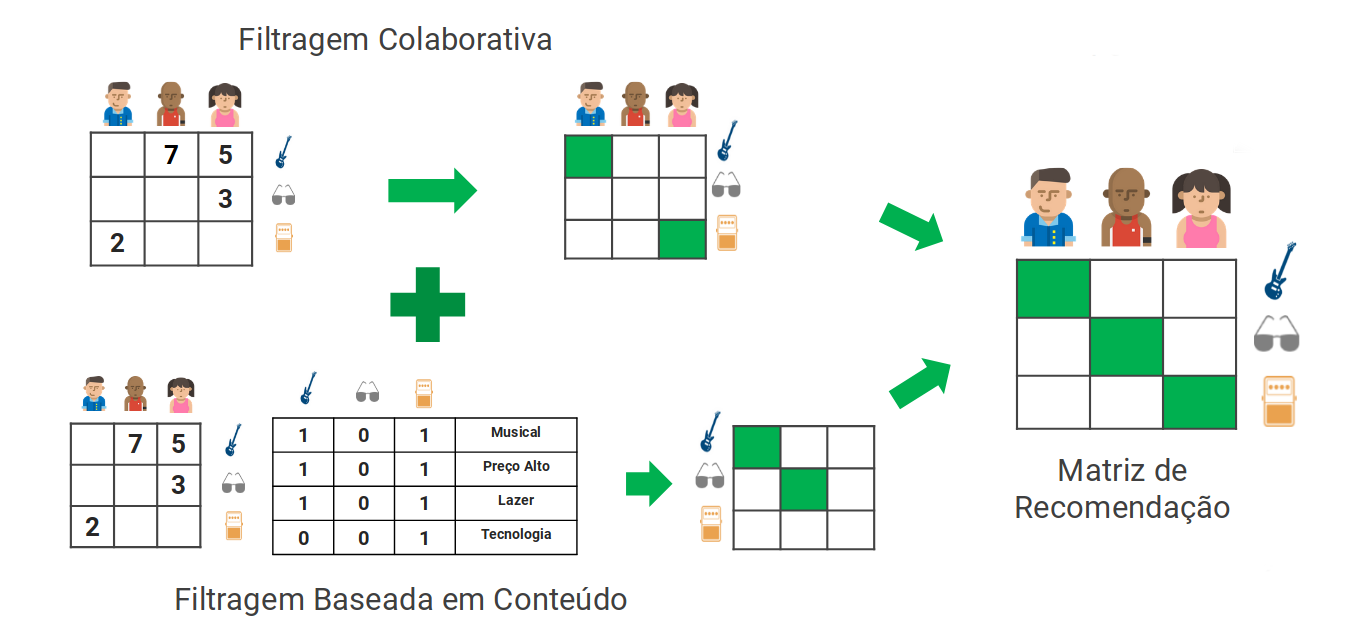
\includegraphics[width=1\linewidth]{imagens/hibrida.png}
	\caption[Exemplo de filtragem híbrida]{Exemplo de filtragem híbrida, adaptado de \cite{araujo2011apprecommender}}
    \label{fig:algoritmohibrido}
\end{figure}

A partir dos resultados gerados em cada uma das abordagens é possível realizar um processo que gere um valor final para a matriz que será recomendada, sendo que, esse processo irá variar de acordo com a abordagem escolhida. 

No trabalho apresentado estão sendo utilizadas as abordagens mista e ponderada para recomendação híbrida.

Na abordagem mista os resultados gerados por ambas as recomendações (colaborativa e baseada em conteúdo) são enviados para o cliente que solicitou a recomendação, conforme figura \ref{fig:algoritmohibridomisto}:

\begin{figure}[H]
	\centering
	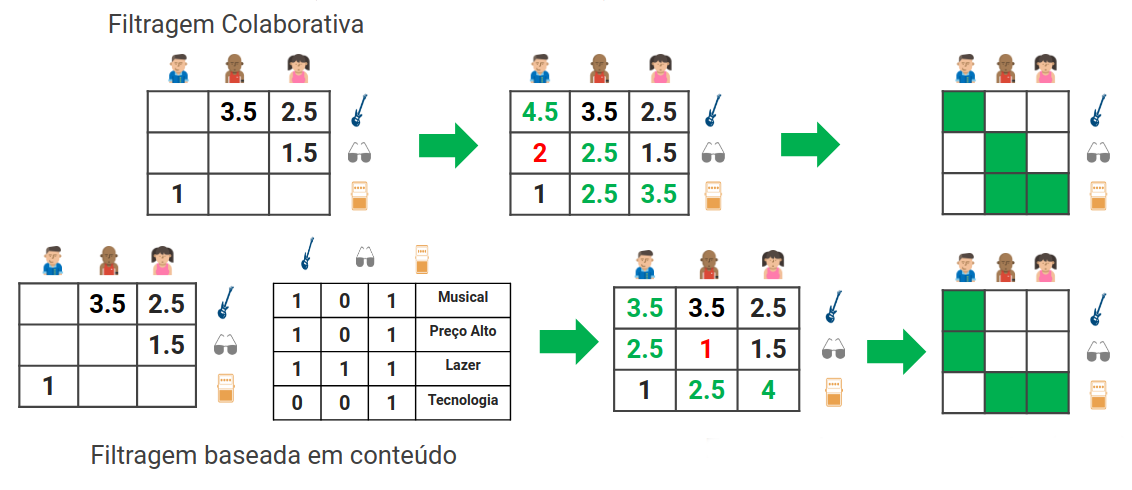
\includegraphics[width=1\linewidth]{imagens/hibridamista.png}
	\caption[Exemplo de filtragem híbrida mista]{Exemplo de filtragem híbrida mista, adaptado de \cite{araujo2011apprecommender}}
    \label{fig:algoritmohibridomisto}
\end{figure}

Para abordagem ponderada, é realizado uma normalização e combinação linear dos dados obtidos nas abordagens colaborativa e baseada em conteúdo, para que então, a partir disso, seja gerado a matriz de recomendação final. Nesse trabalho foi utilizado a média entre valores para o processo de combinação dos resultados, é possível ver um exemplo dessa abordagem na figura \ref{fig:algoritmohibridoponderado}:

\begin{figure}[H]
	\centering
	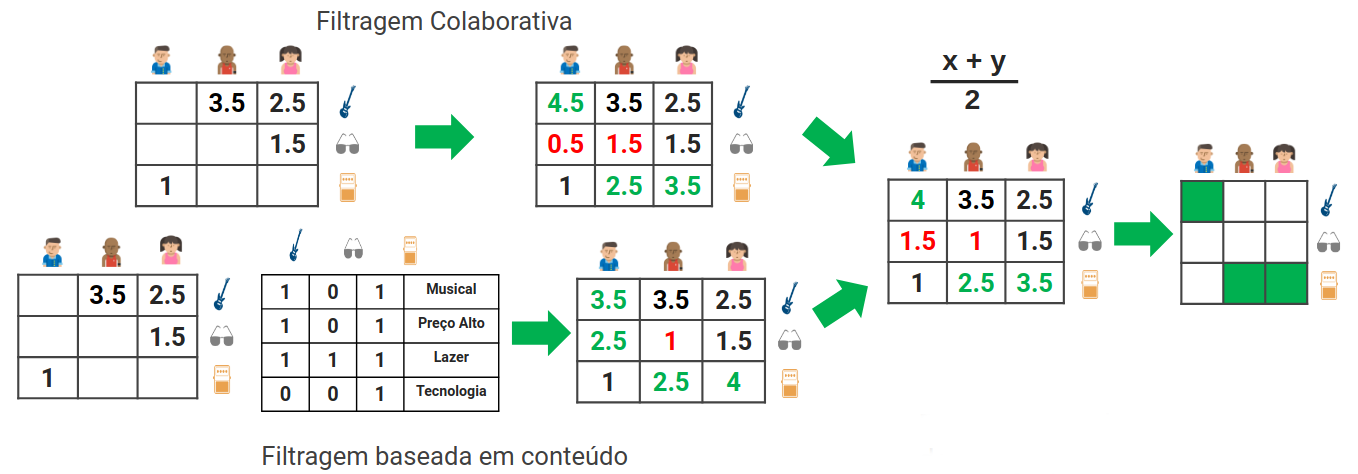
\includegraphics[width=1\linewidth]{imagens/hibridaponderada.png}
	\caption[Exemplo de filtragem híbrida ponderada]{Exemplo de filtragem híbrida ponderada, adaptado de \cite{araujo2011apprecommender}}
    \label{fig:algoritmohibridoponderado}
\end{figure}
%%% ====================================================================
%%% Início da parte textual do documento.


%%% Configuração do espaçamento entre títulos e texto
\setlength{\afterchapskip}{1.5cm minus \baselineskip}


\chapter{Resultados}
\label{cha:resultados}

Esse capítulo contém os resultados da aplicação e dos estudos de casos aplicados.

\section{Aplicação}

\subsection{Diagrama de Classes}

Com auxílio da ferramenta \textit{Astah Community}, foi desenvolvido o seguinte Diagrama de Classes, apresentado na figura \ref{fig:diagramaClasses}:

\begin{figure}[H]
	\centering
	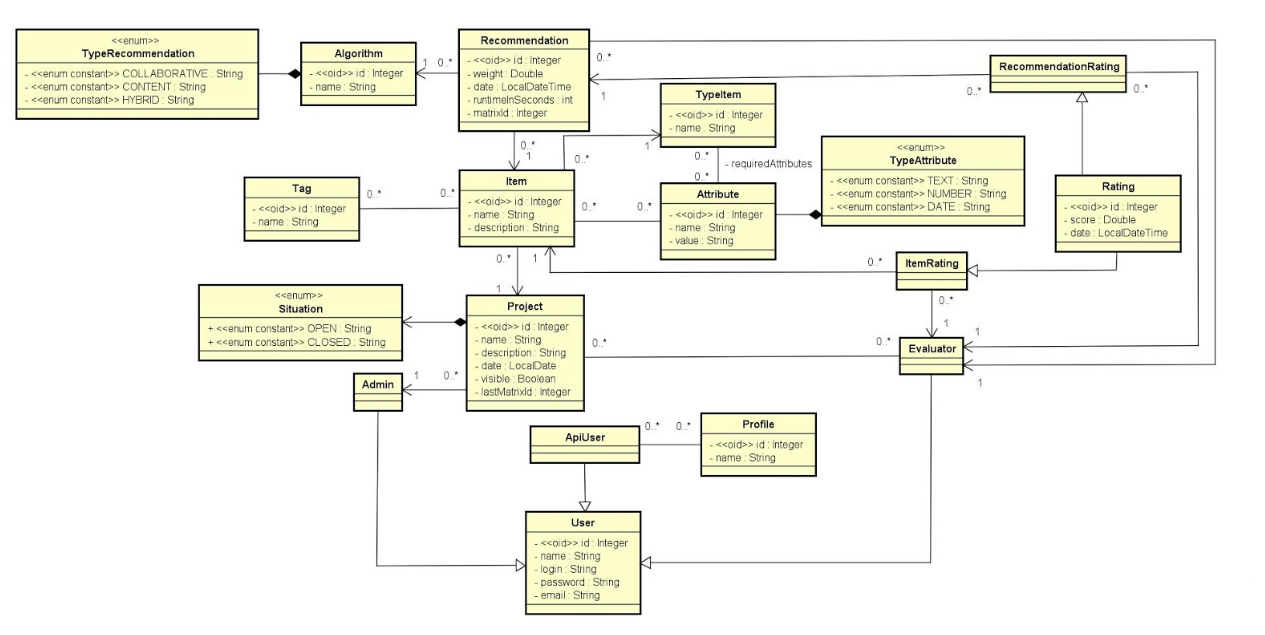
\includegraphics[width=1\linewidth]{imagens/diagramaClasses.PNG}
	\caption[Diagrama de Classes]{Diagrama de Classes}
    \label{fig:diagramaClasses}
\end{figure}

\subsection{API de Recomendação}

Foi desenvolvida uma aplicação backend aberta para uso e modificações. O código fonte de aplicação está disponível no \href{https://github.com/herikLorencao/srh-backend}{GitHub} \footnote{Link do repositório: https://github.com/herikLorencao/srh-backend} podendo ser modificado e adaptado.

Foram desenvolvidos um total de 103 endpoints para a API, que incluem desde cadastros até rotinas de autenticação e recomendação. Todas as rotas estão documentadas e disponíveis no serviço \href{https://documenter.getpostman.com/view/6420672/T1LVA4ST}{Postman} \footnote{Link dos endpoints da API: https://documenter.getpostman.com/view/6420672/T1LVA4ST} para acesso.

Na figura \ref{fig:requisicaoPostman} é possível verificar a documentação das requisições que encontra-se aberta para consulta e uso.

\begin{figure}[H]
	\centering
	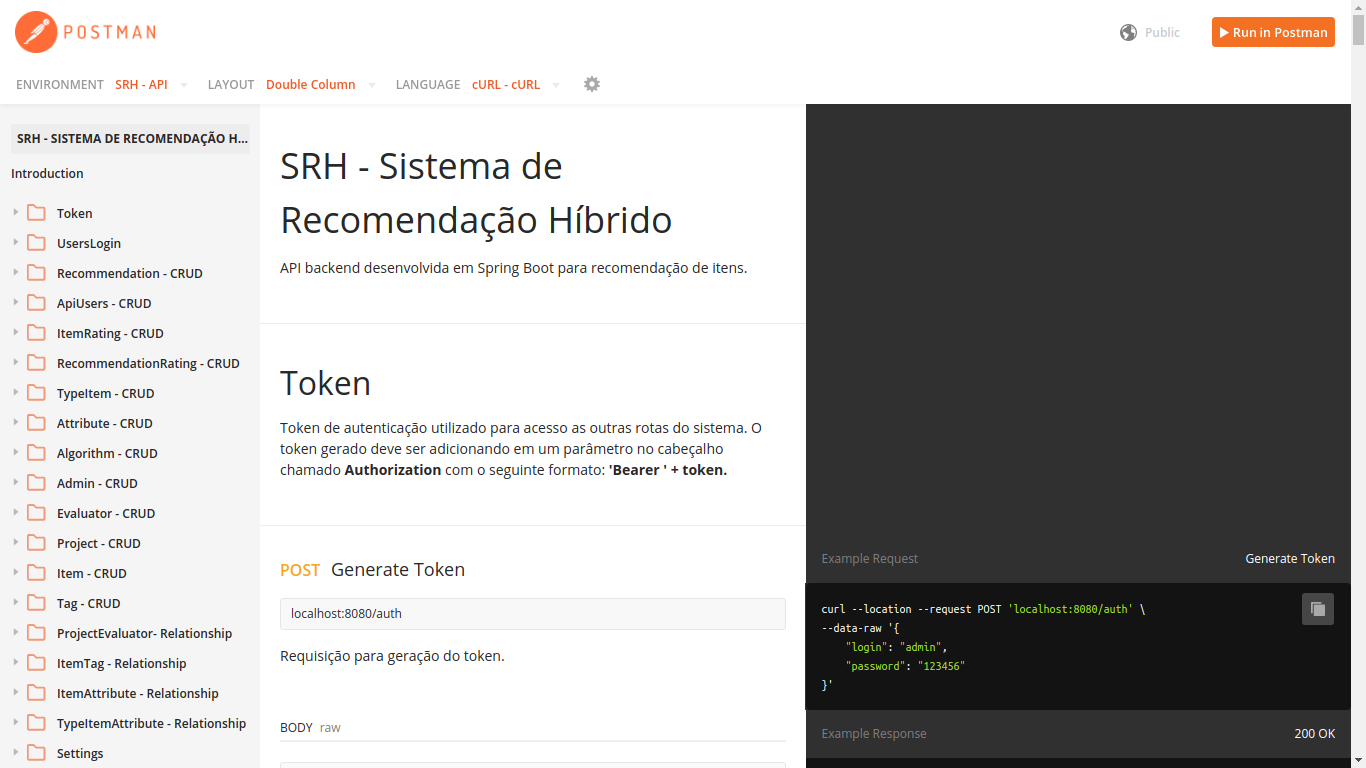
\includegraphics[width=1\linewidth]{imagens/requisicoesPostman.png}
	\caption[Documentação das requisições]{Documentação das requisições}
    \label{fig:requisicaoPostman}
\end{figure}

A API desenvolvida apresenta configuração para uso e distribuição de informação entre diversos clientes, possuindo configurações para tokenização de endpoints e criação de níveis de usuário com privilégios distintos, permitindo um maior controle de acessos aos dados e recursos do sistema.

\textbf{Concorrência}

Foi desenvolvido um endpoint que possibilita o cálculo das recomendações de maneira concorrente, a partir do uso de funções assíncronas no framework \textbf{Spring Boot}.

Como base para desenvolvimento foi utilizado o projeto oferecido pela documentação do \textbf{Spring} \footnote{Disponível em: https://spring.io/guides/gs/async-method/} que demonstra o uso do sistema de concorrência e como essa técnica pode permitir a melhoria no tempo de execução de códigos complexos.
\newline

Para os testes de velocidade, foi utilizado o seguinte ambiente para execução, mostrado na tabela \ref{tableref:ambienteTeste}:

\begin{table}[H]
\centering
\begin{tabular}{|c|c|}
\hline
\textbf{Componentes} & \textbf{Informações} \\ \hline
Número Processadores & 2                               \\ \hline
Número de Threads    & 4                               \\ \hline
Mémoria RAM          & 8 GB                            \\ \hline
Armazenamento        & 1 TB HDD                        \\ \hline
\end{tabular}
\caption{Ambiente de execução dos testes}
\label{tableref:ambienteTeste}
\end{table}

Com os ambientes definidos, foram executadas três requisições para cada abordagem de recomendação nos servidores onde foi mapeado o tempo de resposta para o cliente de cada recomendação. Com os dados definidos, foi realizada uma média aritmética dos valores, resultando nos dados definidos nas tabelas \ref{tableref:execucaoRecomendacaoSemConcorrencia} e \ref{tableref:execucaoRecomendacaoComConcorrencia}. Como dados para análise foram utilizados as informações coletadas no estudo de caso educacional.

\begin{table}[H]
\centering
\begin{tabular}{|c|c|}
\hline
\multicolumn{2}{|c|}{\textbf{Tempo de Recomendação - Sem Concorrência}} \\ \hline
\textbf{Informações}                 & \textbf{Tempo de Execução (s)}    \\ \hline
Recomendação Colaborativa            & 2,88                               \\ \hline
Recomendação Baseada em Conteúdo     & 3,02                               \\ \hline
Recomendação Híbrida Ponderada       & 20,64                              \\ \hline
Recomendação Híbrida Mista           & 5,64                               \\ \hline
\end{tabular}
\caption{Tempo de execução das recomendações: sem concorrência}
\label{tableref:execucaoRecomendacaoSemConcorrencia}
\end{table}

\begin{table}[H]
\centering
\begin{tabular}{|c|c|}
\hline
\multicolumn{2}{|c|}{\textbf{Tempo de Recomendação - Com Concorrência}} \\ \hline
\textbf{Informações}                 & \textbf{Tempo de Execução (s)}    \\ \hline
Recomendação Colaborativa            & 30,41                              \\ \hline
Recomendação Baseada em Conteúdo     & 26,78                               \\ \hline
Recomendação Híbrida Ponderada       & 180                              \\ \hline
Recomendação Híbrida Mista           & 32,81                              \\ \hline
\end{tabular}
\caption{Tempo de execução das recomendações: com concorrência}
\label{tableref:execucaoRecomendacaoComConcorrencia}
\end{table}

Infelizmente, devido ao nível de complexidade do algoritmo, principalmente em relação ao acesso aos dados pelo ORM \textit{(Object Relational Mapper)} foi observado uma perca de performance significativa no uso do algoritmo de maneira concorrente. Outro fator que deve ser levado em consideração, é em relação ao \textit{overhead} gerado pelo processo de concorrência, visto que vários processos também precisar ser iniciados e manipulados para que o processo de recomendação ocorra, fazendo com que o tempo de execução possa ser prejudicado.

Para verificar os resultados com um volume maior de dados, foram gerados diversos cadastros randômicos no sistema fazendo com que se atingisse o valor de cerca de 2000 recomendações. De maneira geral, os problemas do ORM ainda persistiram, fazendo com que não houvesse melhorias significativas no desempenho do sistema, mesmo com um volume de dados maior.

Para um melhor resultado no processo de concorrência torna-se necessário um conhecimento mais profundo acerca do gerenciamento de processos e escalonamento embutido no Spring, além de ajustes na arquitetura e modelagem do sistema procurando separar logicamente as classes de recomendação do restante do projeto.

Como alternativa para desenvolvimento de um sistema concorrente pode ser interessante avaliar o uso do Spring Reactive \footnote{Documentação disponível em: https://spring.io/reactive}, uma vez que essa ferramenta apresenta diversos recursos que visam permitir e facilitar o desenvolvimento de sistemas que utilizem conceitos concorrentes.

\textbf{Matriz de recomendação offline}

Como forma de buscar uma maneira de acesso mais rápido às recomendações, foi desenvolvido um endpoint para recomendação offline que acaba utilizando-se de dados salvos anteriormente para busca das recomendações, evitando o processamento e cálculo das recomendações novamente, o que acaba por oferecer um menor tempo de resposta para os usuários.

Vale ressaltar que esse processo utiliza-se das recomendações já salvas no banco de dados da aplicação, fazendo com que esses dados não sejam os mais atuais possíveis. Esse fator negativo é recompensado pelo menor tempo de resposta do servidor, além da redução de processamento e acesso ao banco de dados pelo sistema.

Para realização dos testes de performance, foram utilizados os mesmos ambientes de teste informados na seção de resultados relativa à concorrência. O processo de mapeamento dos dados foi semelhante, capturando o tempo de resposta das requisições e realizando a média aritmética dos resultados.

Desse modo, foi possível definir os seguintes dados apresentados na tabela \ref{tableref:execucaoRecomendacaoMatrix}:

\begin{table}[H]
\centering
\begin{tabular}{|c|c|c|}
\hline
\multicolumn{3}{|c|}{\textbf{Tempo de Execução das Recomendações em segundos}}  \\ \hline
\textbf{Abordagem}  & \textbf{Com matrix offline} & \textbf{Sem matrix offline} \\ \hline
Colaborativa        & 1,96                        & 2,88                        \\ \hline
Baseada em Conteúdo & 1,60                        & 3,02                        \\ \hline
Híbrida Ponderada   & 1,31                        & 20,64                       \\ \hline
Híbrida Mista       & 1,32                        & 5,64                        \\ \hline
\end{tabular}
\caption{Comparação da execução utilizando a técnica de matrix de recomendação offline}
\label{tableref:execucaoRecomendacaoMatrix}
\end{table}

\subsection{Cliente Administrativo}

Para acesso e manipulação dos recursos do sistema foi desenvolvido um cliente administrativo para acesso na WEB\footnote{Link do repositório: https://github.com/herikLorencao/srh-client-admin}. Nele é possível cadastrar, alterar, visualizar e remover os principais recursos do sistema, permitindo que um usuário com perfil de administrador possa criar e manipular diversos projetos. Nas figuras \ref{fig:clienteAdminLogin}, \ref{fig:clienteAdminProjeto}, \ref{fig:clienteAdminCriarProjeto}, \ref{fig:clienteAdminUsuarios}, \ref{fig:clienteAdminAvaliacoes}, \ref{fig:clienteAdminRecomendacoes} e \ref{fig:clienteAdminUsuarioAPI} é possível visualizar algumas das telas do sistema.

\begin{figure}[H]
	\centering
	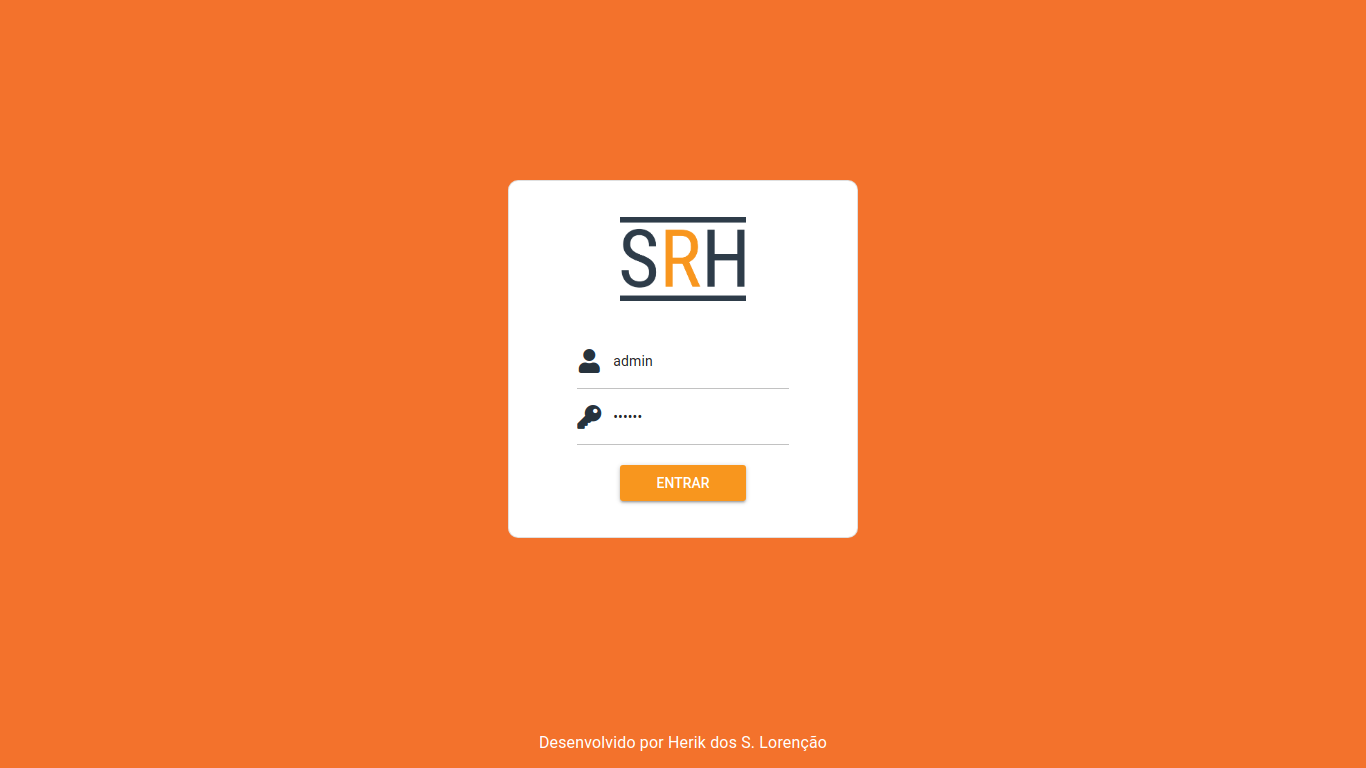
\includegraphics[width=.9\linewidth]{imagens/adminLogin.png}
	\caption[Cliente Administrativo: Login]{Cliente Administrativo: Login}
    \label{fig:clienteAdminLogin}
\end{figure}

\begin{figure}[H]
	\centering
	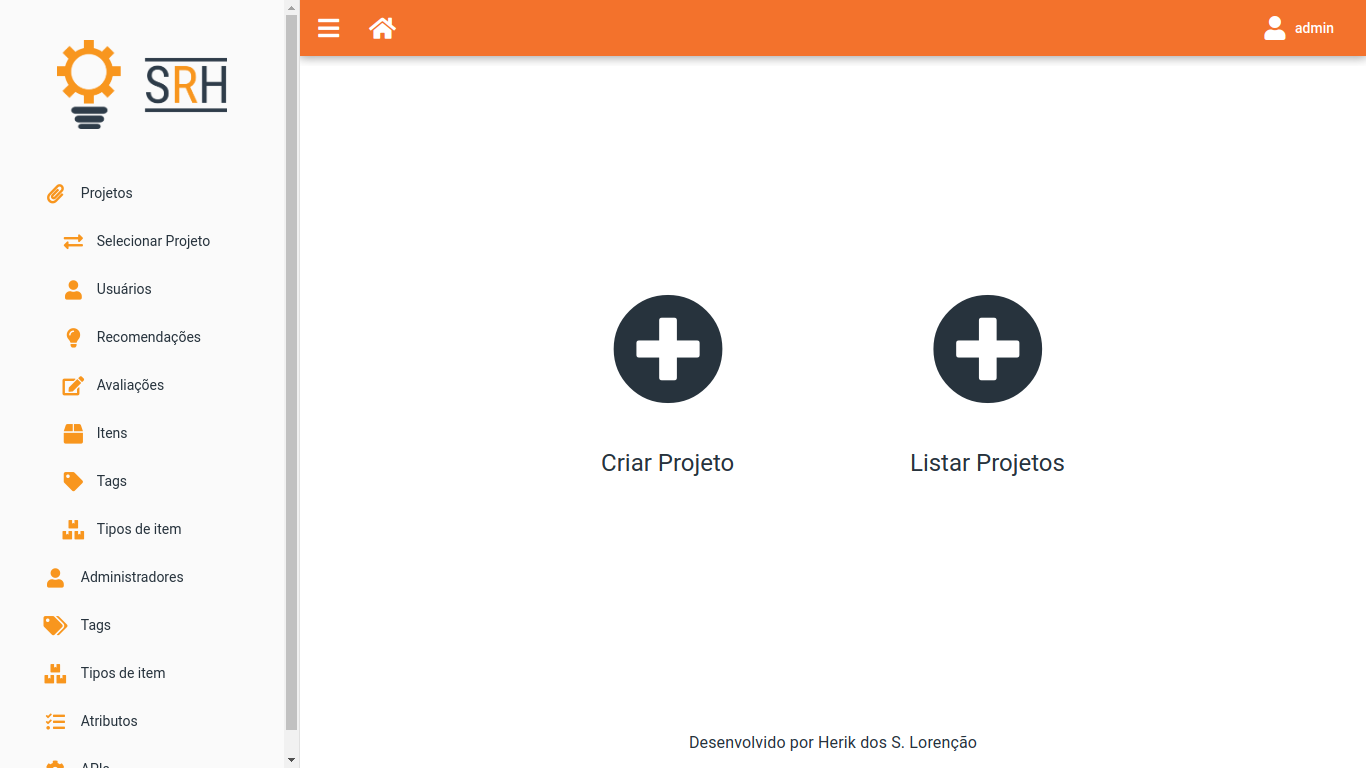
\includegraphics[width=.9\linewidth]{imagens/adminCriarProjeto.png}
	\caption[Cliente Administrativo: Projeto]{Cliente Administrativo: Projeto}
    \label{fig:clienteAdminProjeto}
\end{figure}

\begin{figure}[H]
	\centering
	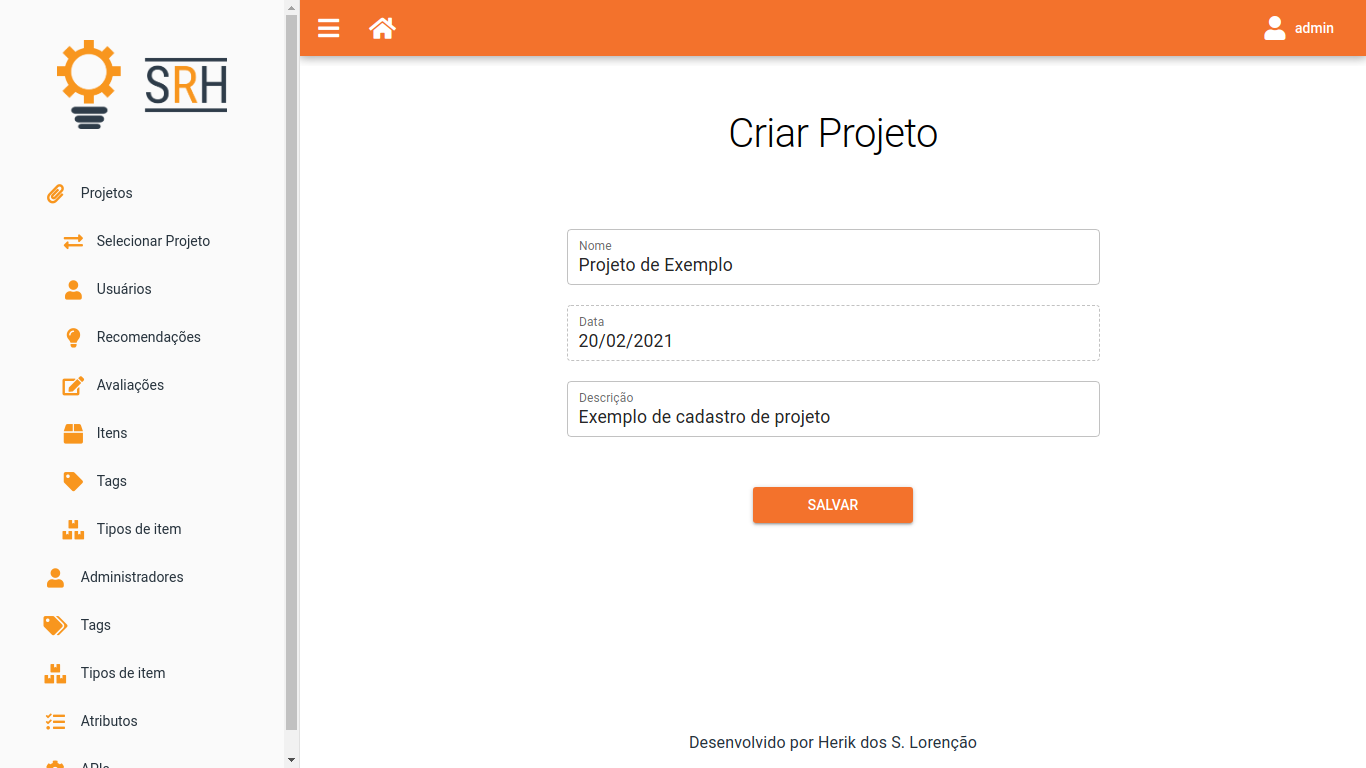
\includegraphics[width=.9\linewidth]{imagens/adminCriarProjetoForm.png}
	\caption[Cliente Administrativo: Criar Projeto]{Cliente Administrativo: Criar Projeto}
    \label{fig:clienteAdminCriarProjeto}
\end{figure}

\begin{figure}[H]
	\centering
	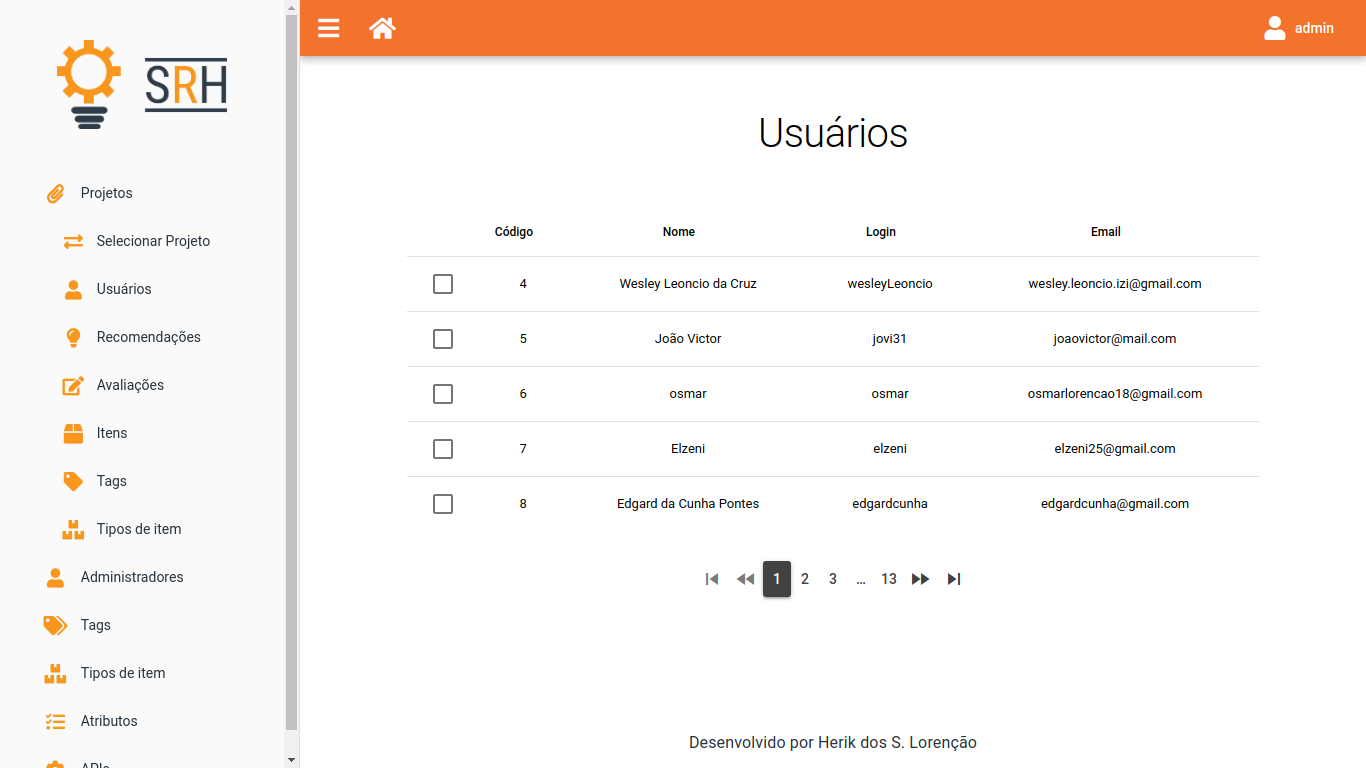
\includegraphics[width=.9\linewidth]{imagens/adminUsuarios.png}
	\caption[Cliente Administrativo - Usuários]{Cliente Administrativo: Usuários}
    \label{fig:clienteAdminUsuarios}
\end{figure}

\begin{figure}[H]
	\centering
	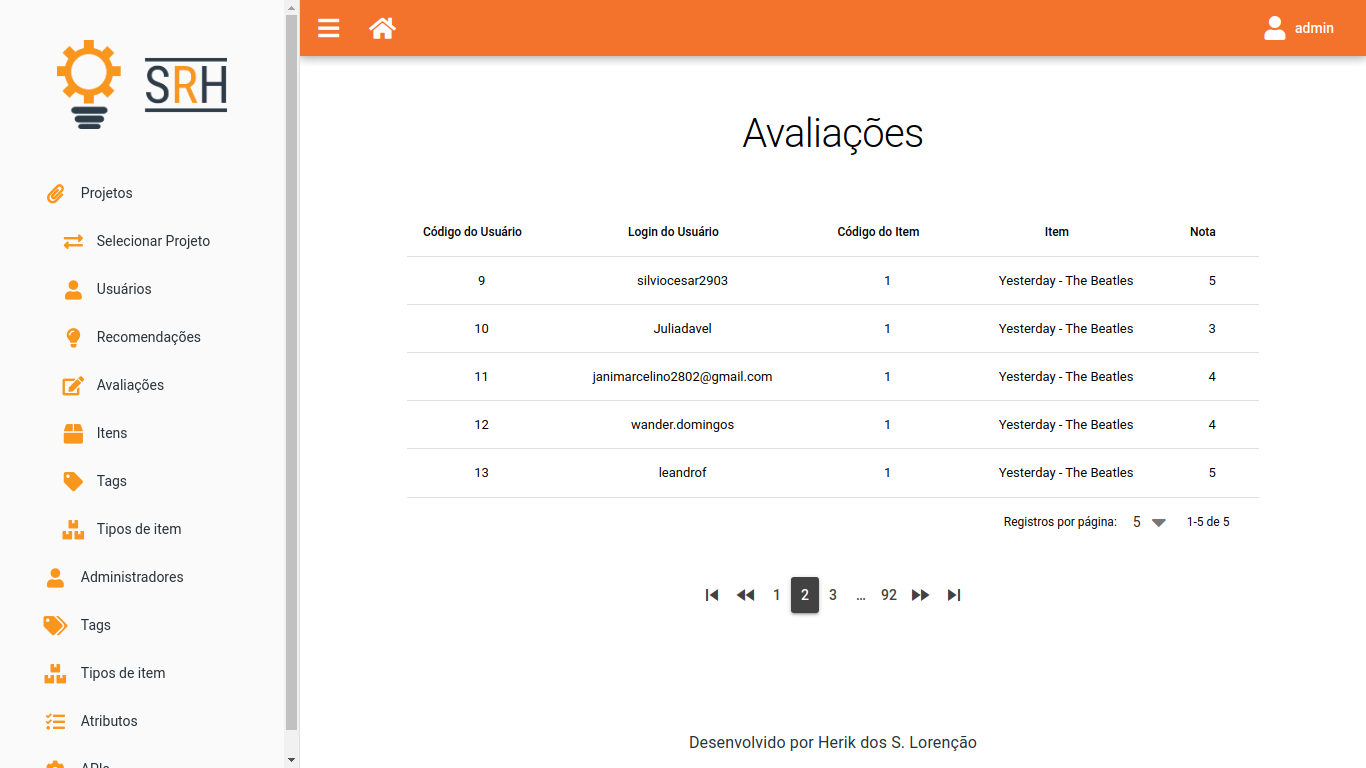
\includegraphics[width=.9\linewidth]{imagens/adminAvaliacoes.png}
	\caption[Cliente Administrativo: Avaliações]{Cliente Administrativo: Avaliações}
    \label{fig:clienteAdminAvaliacoes}
\end{figure}

\begin{figure}[H]
	\centering
	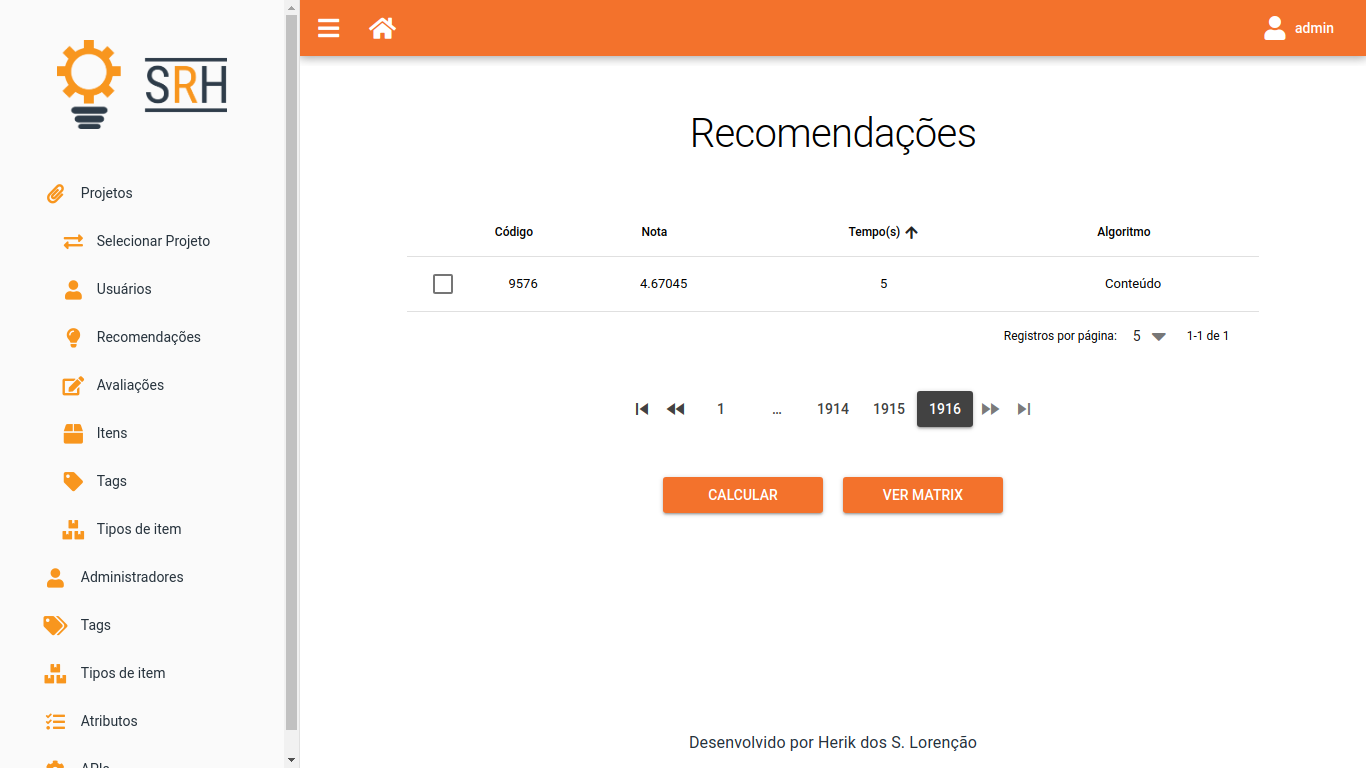
\includegraphics[width=.9\linewidth]{imagens/adminRecomendacoes.png}
	\caption[Cliente Administrativo: Recomendações]{Cliente Administrativo: Recomendações}
    \label{fig:clienteAdminRecomendacoes}
\end{figure}

\begin{figure}[H]
	\centering
	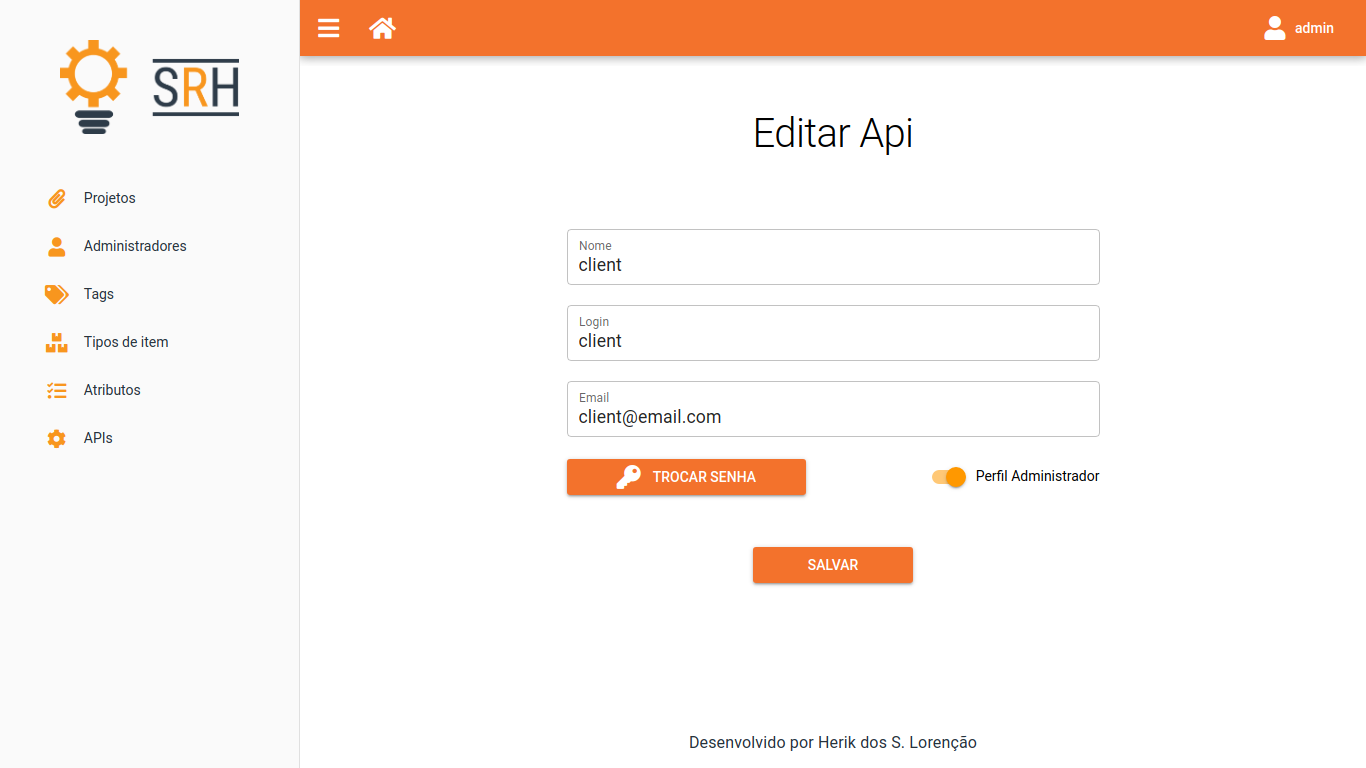
\includegraphics[width=.9\linewidth]{imagens/adminApi.png}
	\caption[Cliente Administrativo - Login]{Cliente Administrativo: Editar Usuário de API}
    \label{fig:clienteAdminUsuarioAPI}
\end{figure}

\subsection{Cliente de Recomendação}

Para que os avaliadores possam avaliar os itens em seus respectivos projetos foi desenvolvido uma aplicação cliente de recomendação\footnote{Link do repositório: https://github.com/herikLorencao/srh-client}, que permite o cadastro e acesso de um avaliador a um determinado projeto. Nas figuras \ref{fig:clienteLogin}, \ref{fig:clienteInicio}, \ref{fig:clienteAvaliacao}, \ref{fig:clienteAvaliacaoFinalizar} e \ref{fig:clienteEditarPerfil} pode-se visualizar algumas telas do sistema.

\begin{figure}[H]
	\centering
	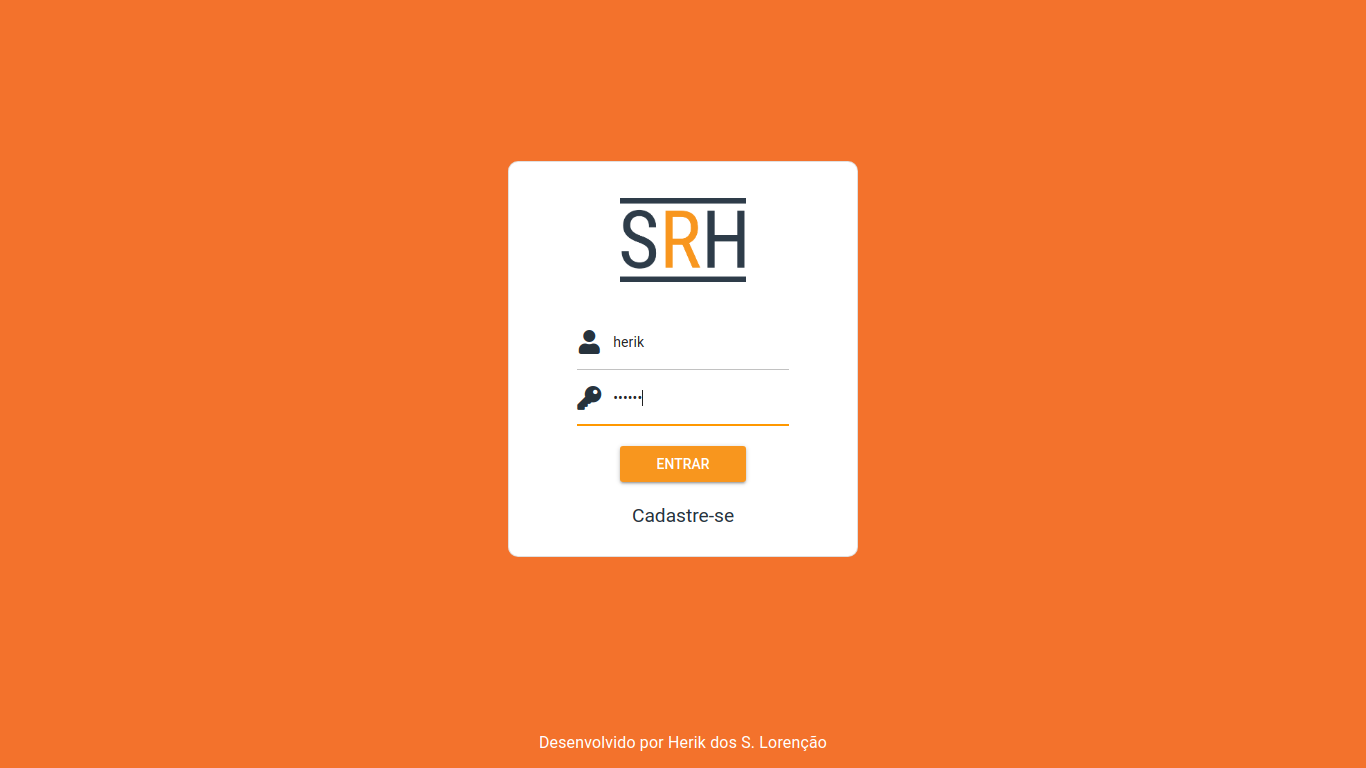
\includegraphics[width=.9\linewidth]{imagens/clientLogin.png}
	\caption[Cliente de Recomendação: Login]{Cliente de Recomendação: Login}
    \label{fig:clienteLogin}
\end{figure}

\begin{figure}[H]
	\centering
	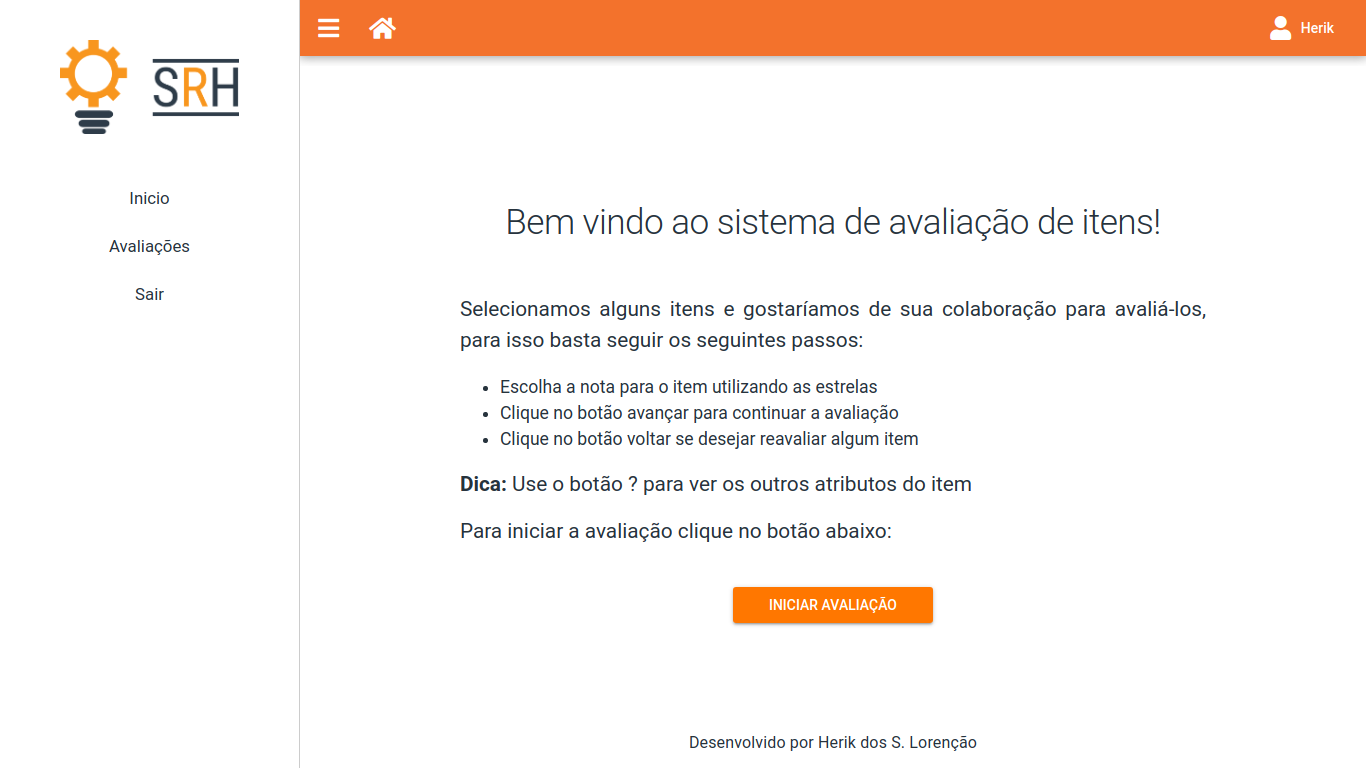
\includegraphics[width=.9\linewidth]{imagens/clientInicio.png}
	\caption[Cliente de Recomendação: Inicio]{Cliente de Recomendação: Inicio}
    \label{fig:clienteInicio}
\end{figure}

\begin{figure}[H]
	\centering
	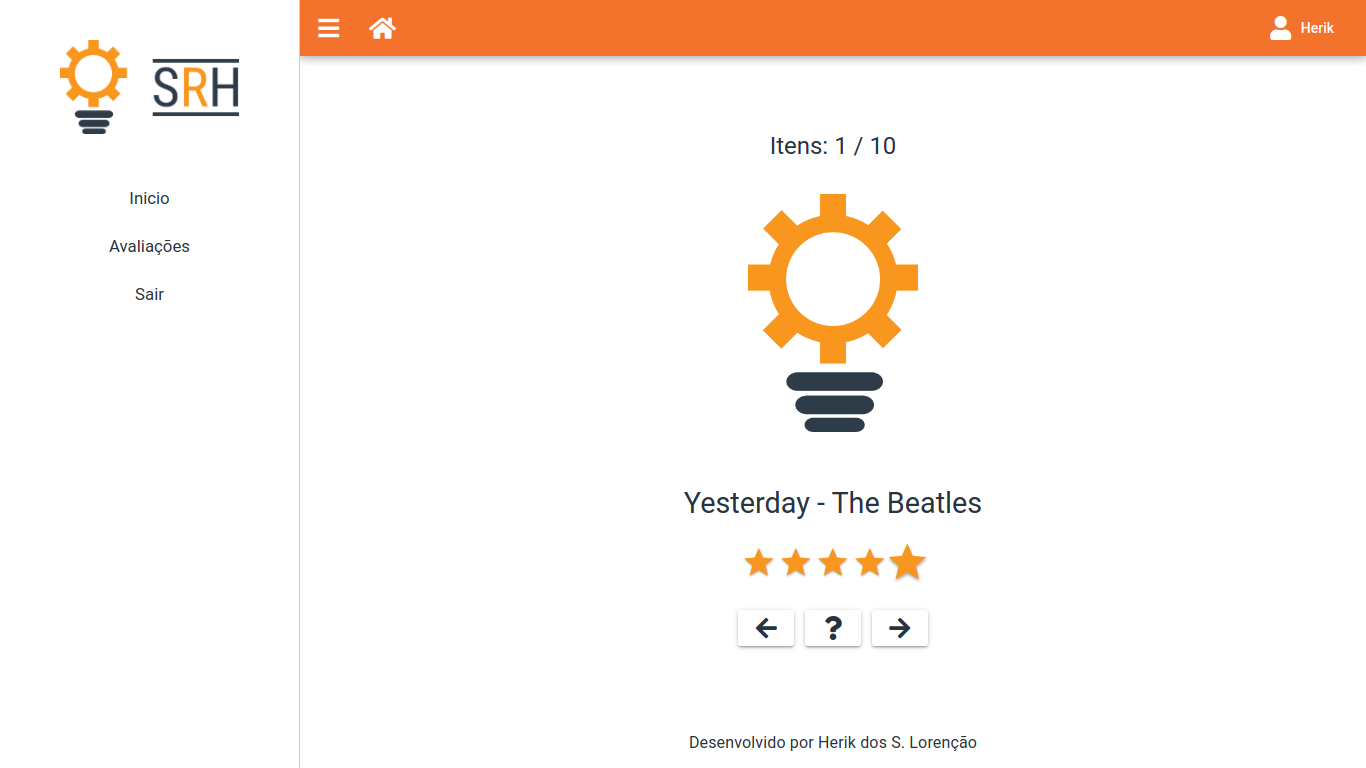
\includegraphics[width=.9\linewidth]{imagens/clientAvaliacao.png}
	\caption[Cliente de Recomendação: Avaliação]{Cliente de Recomendação: Avaliação}
    \label{fig:clienteAvaliacao}
\end{figure}

\begin{figure}[H]
	\centering
	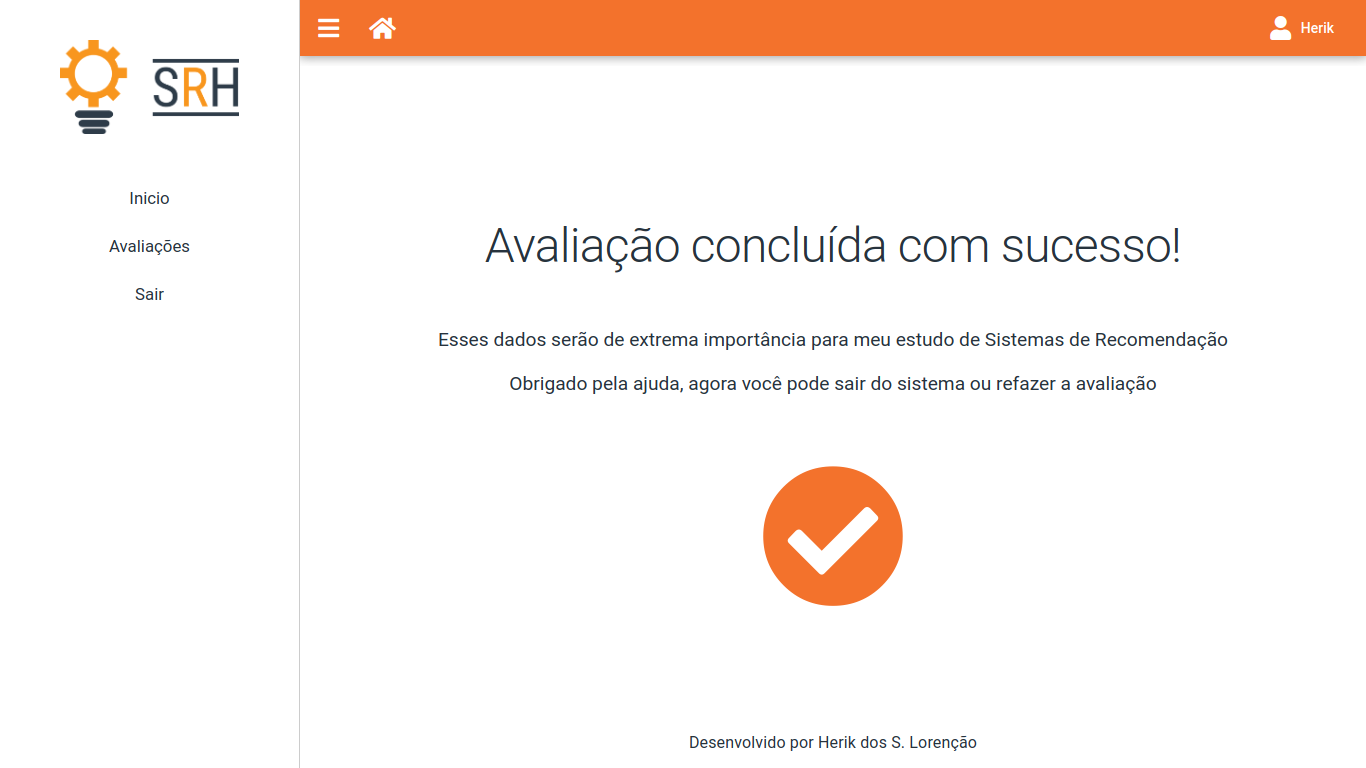
\includegraphics[width=.9\linewidth]{imagens/clientFinalizar.png}
	\caption[Cliente de Recomendação: Finalizar Avaliação]{Cliente de Recomendação: Finalizar Avaliação}
    \label{fig:clienteAvaliacaoFinalizar}
\end{figure}

\begin{figure}[H]
	\centering
	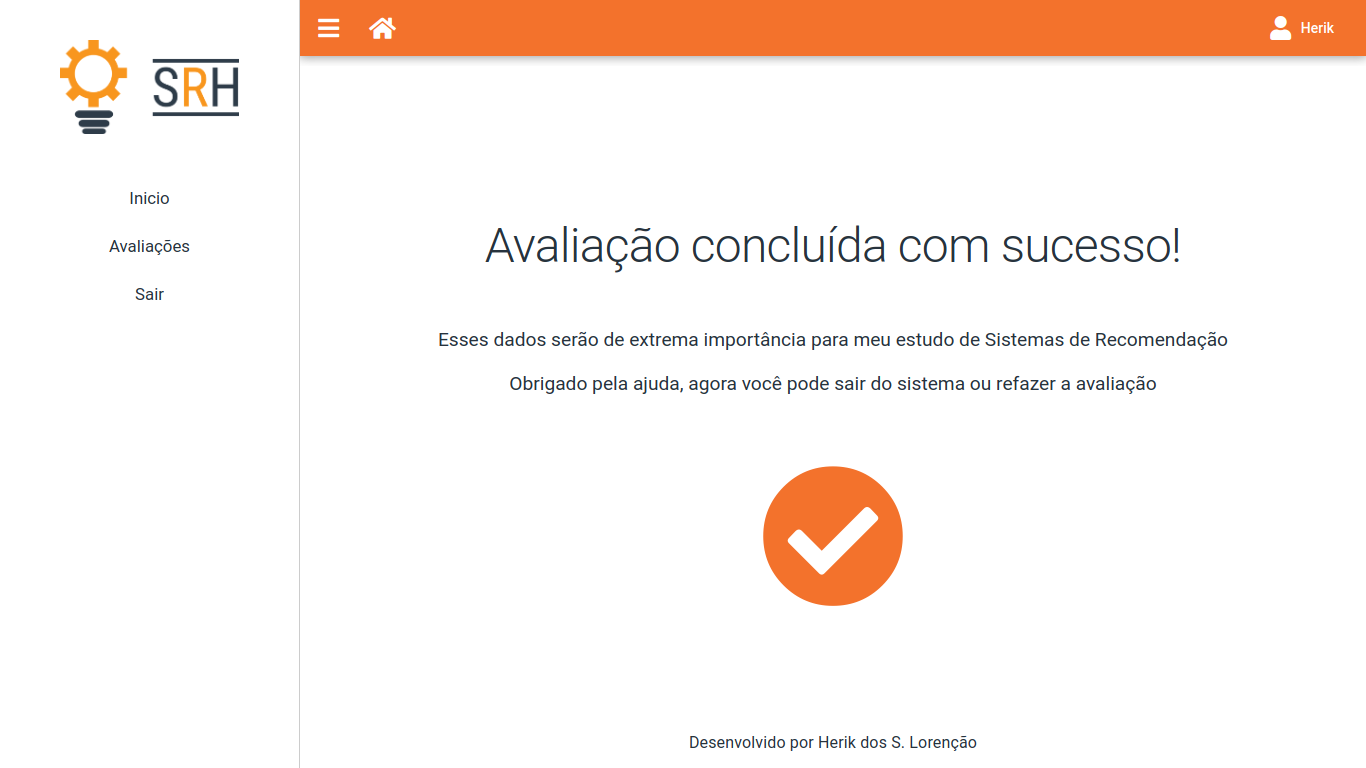
\includegraphics[width=.9\linewidth]{imagens/clientFinalizar.png}
	\caption[Cliente de Recomendação: Editar Perfil]{Cliente de Recomendação: Editar Perfil}
    \label{fig:clienteEditarPerfil}
\end{figure}

\section{Estudo de Caso: Educacional}

\subsection{Contexto}

O intuito deste estudo de caso foi recomendar exercícios aos alunos que pudessem auxiliar significativamente com seu aprendizado no conteúdo estudado.

Para desenvolvendo do estudo de caso, foi selecionada uma turma do curso técnico de Informática Integrado ao Ensino Médio do IFES - Campus Cachoeiro de Itapemirim. O objetivo era o de realizar perguntas relacionadas ao tema de estruturas de controle, na disciplina de Programação I.

Desse modo, o questionário foi aplicado na turma sendo pedido que todos os alunos respondessem todas as perguntas. Para avaliar a assertividade do sistema de recomendação, foram retiradas, de forma aleatória, um conjunto de 0 a 4 respostas de cada aluno, tendo como objetivo criar um ambiente para recomendação onde fosse possível avaliar a taxa de acerto das notas recomendadas.

Na tabela \ref{tableref:dadosEstudoCasoEducacional} é possível visualizar os dados acerca da pesquisa realizada:

\begin{table}[H]
\centering
\begin{tabular}{|c|c|}
\hline
\textbf{Itens}          & \textbf{Quantidade} \\ \hline
Número de alunos        & 29                  \\ \hline
Número de perguntas     & 9                   \\ \hline
Número de avaliações    & 214                 \\ \hline
Número de tags          & 9                   \\ \hline
Número de recomendações & 47                  \\ \hline
\end{tabular}
\caption{Dados do estudo de caso educacional}
\label{tableref:dadosEstudoCasoEducacional}
\end{table}

\subsection{Análise Descritiva}

Utilizando-se da estatística descritiva, pode-se avaliar a porcentagem de recomendações que foram aceitas pelos usuários do sistema, verificando, desse modo, sua taxa de acerto. Na figura \ref{fig:analiseDescritiva}, é possível avaliar os resultados obtidos nas recomendações como também as notas avaliadas pelos alunos para cada pergunta. A partir desses dados é possível realizar o processo de estatística descritiva.

\begin{figure}[H]
	\centering
	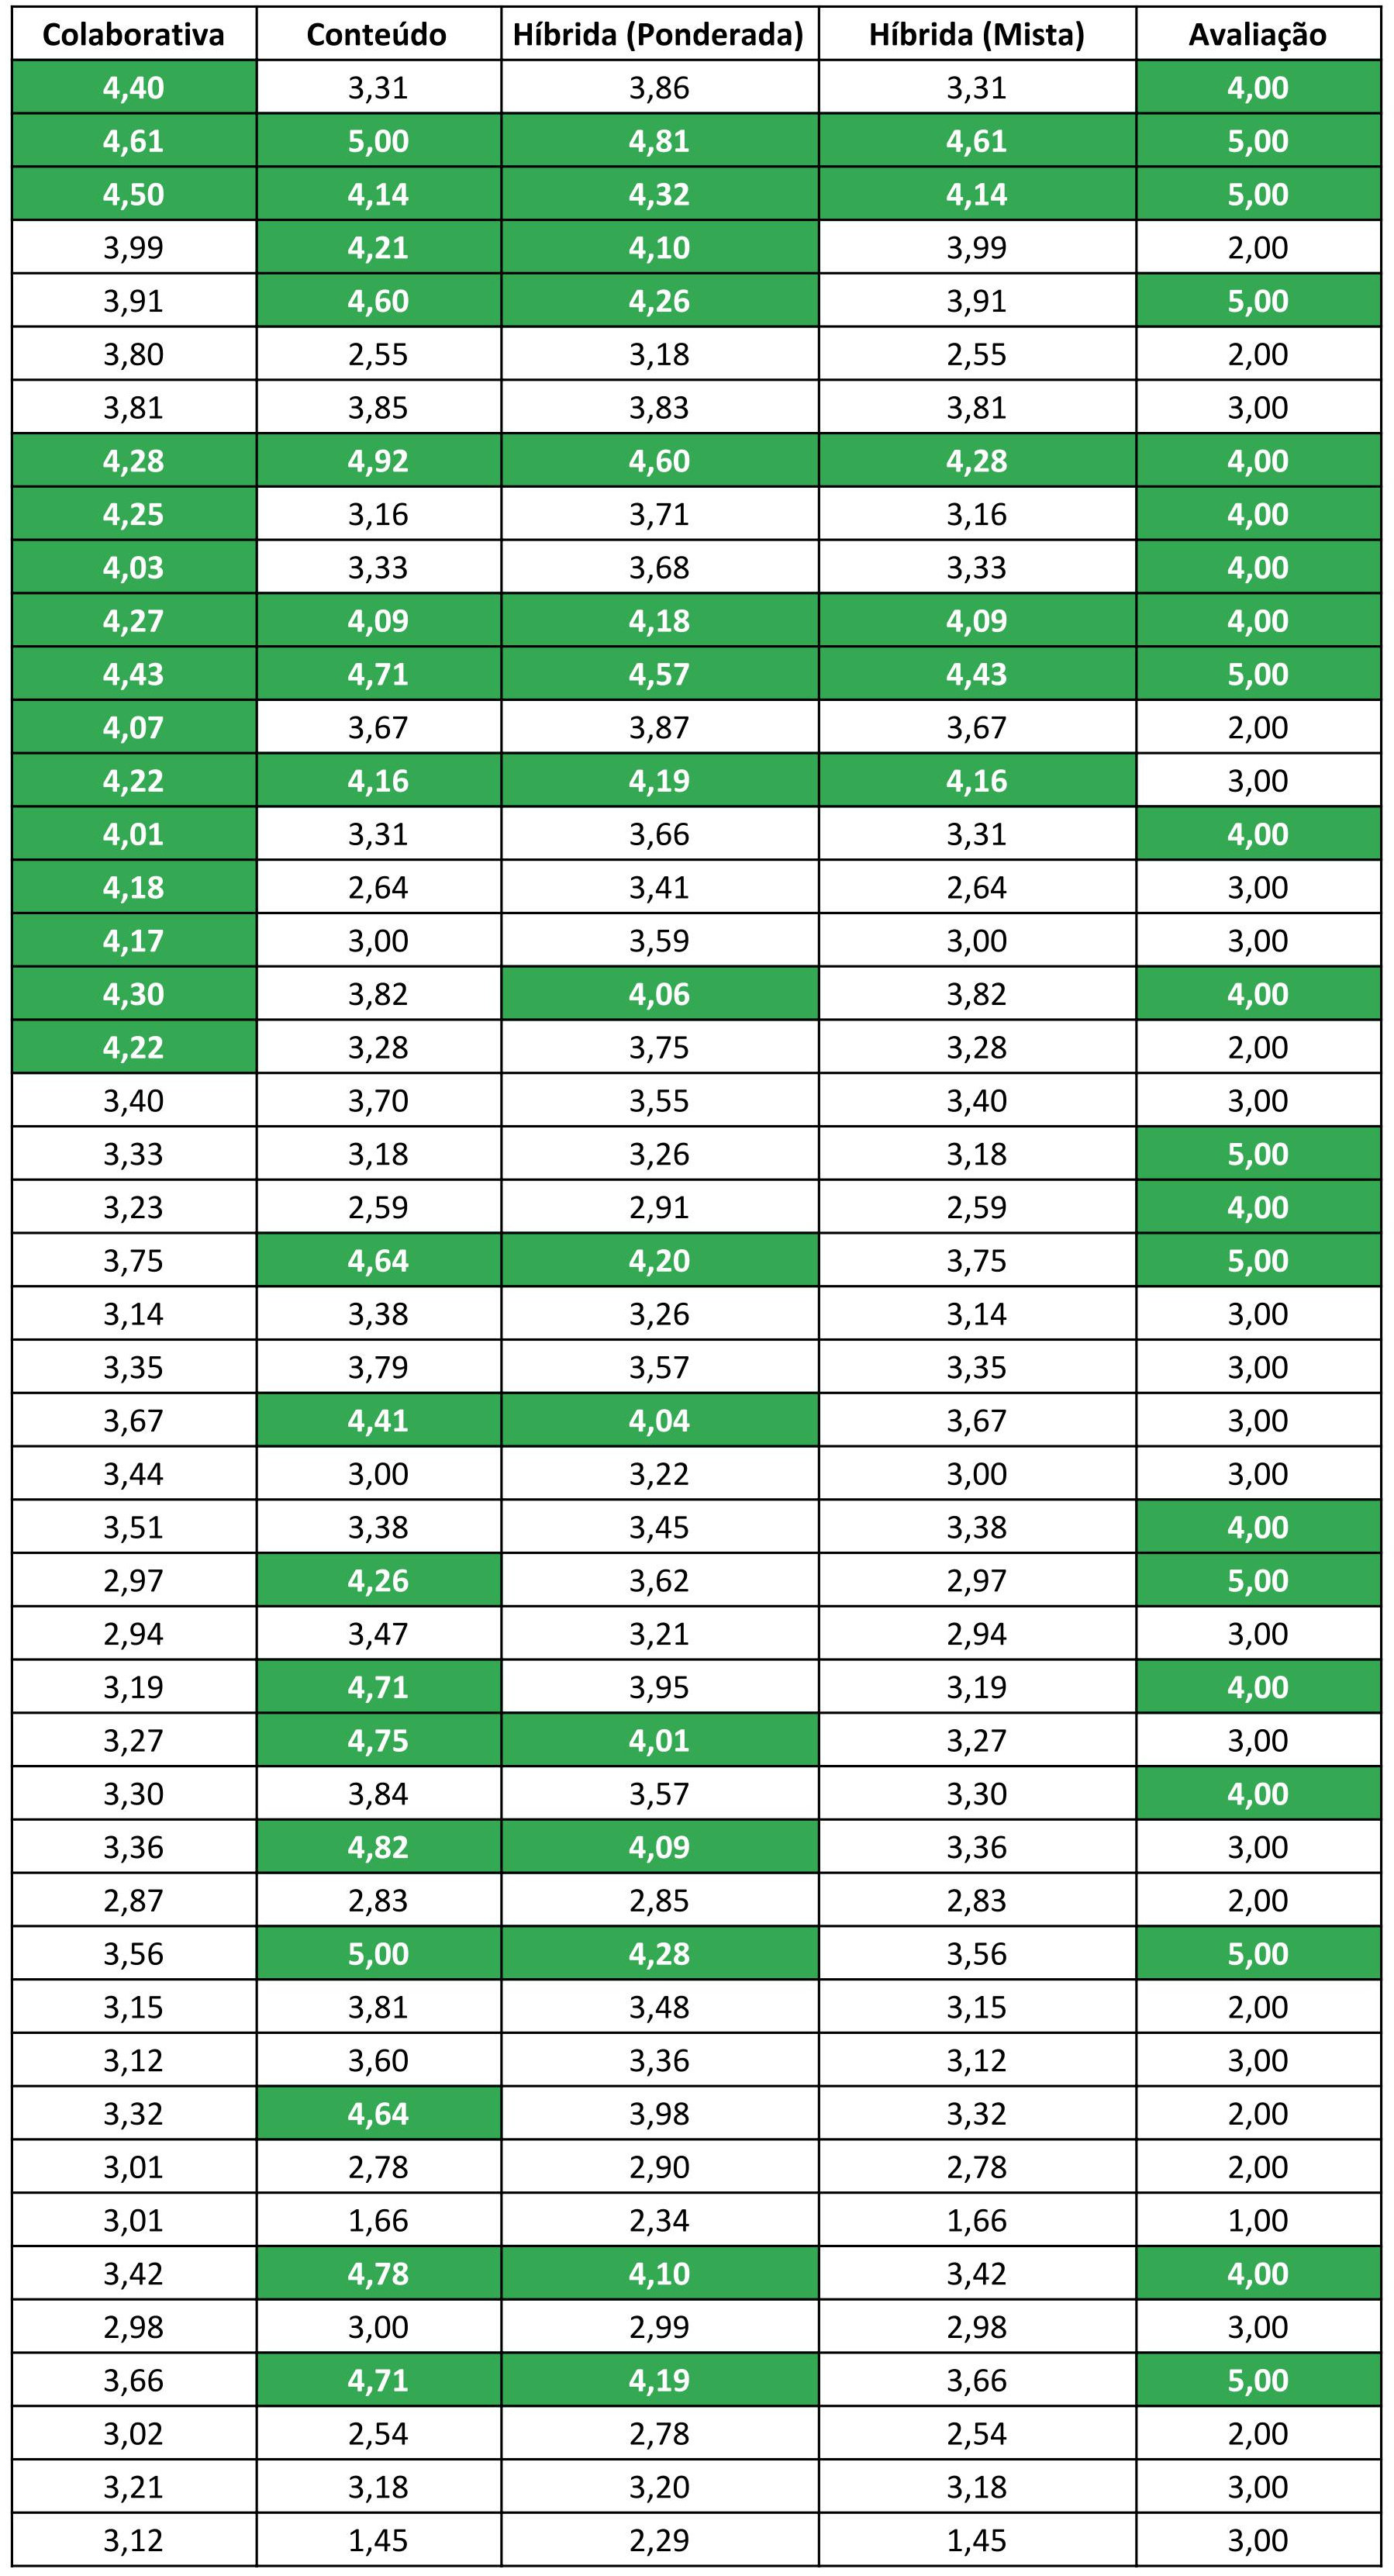
\includegraphics[width=0.8\linewidth]{imagens/estatisticaDescritiva.jpg}
	\caption[Estatística Descritiva]{Estatística Descritiva}
    \label{fig:analiseDescritiva}
\end{figure}

Avaliando as células marcadas na cor verde na figura \ref{fig:analiseDescritiva}, que representam os itens recomendados (notas maiores que o ponto de corte, definido como 4), é possível visualizar a quantidade de acertos e erros das abordagens de recomendação em relação as notas avaliadas pelos usuários. Esses dados são apresentados na figura \ref{fig:analiseDescritivaTaxas}:

\begin{figure}[H]
	\centering
	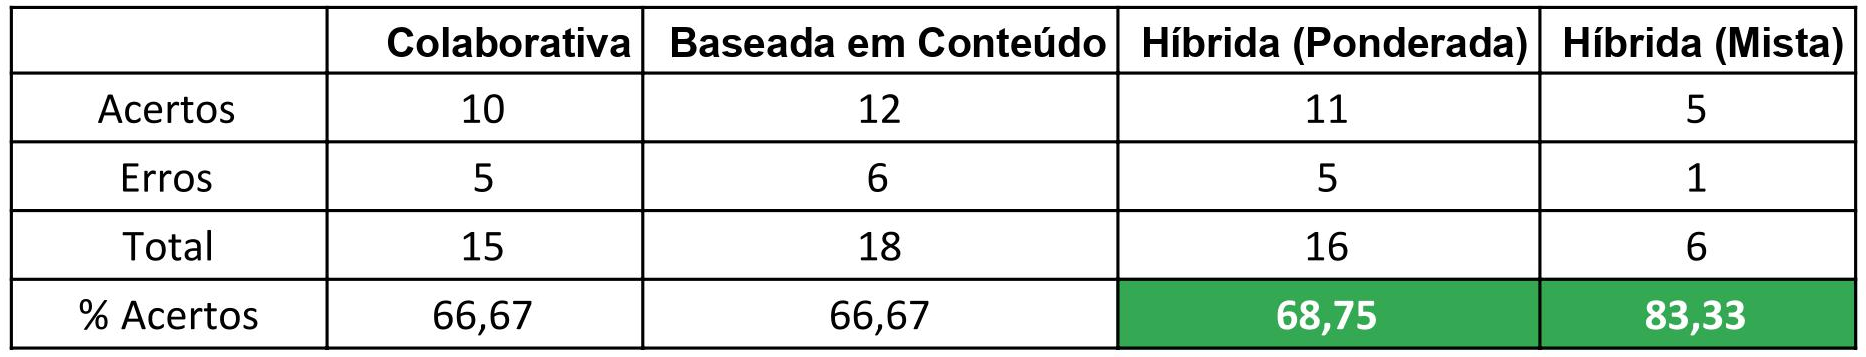
\includegraphics[width=.9\linewidth]{imagens/analiseDescritivaTaxas.jpg}
	\caption[Taxas da Estatística Descritiva]{Taxas da Estatística Descritiva}
    \label{fig:analiseDescritivaTaxas}
\end{figure}

A partir dos dados disponíveis na figura \ref{fig:analiseDescritivaTaxas}, conclui-se que as abordagens híbridas (marcadas com a cor verde) obtiveram um resultado superior as abordagens colaborativas e baseada em conteúdo no estudo analisado. Vale ressaltar o resultado obtido na abordagem híbrida mista, que apresentou um resultado 16,66\% superior as abordagens não híbridas.

\subsection{Teste T de Student}

Como forma de avaliar os resultados sobre outra perspectiva e metodologia, foram realizados os testes t de Student que representam outra forma de análise estatística. Nesse tipo de análise, é buscado verificar a diferença entre as médias das recomendações e as avaliações dos estudantes, buscando a menor divergência possível entre os resultados.

\begin{figure}[H]
	\centering
	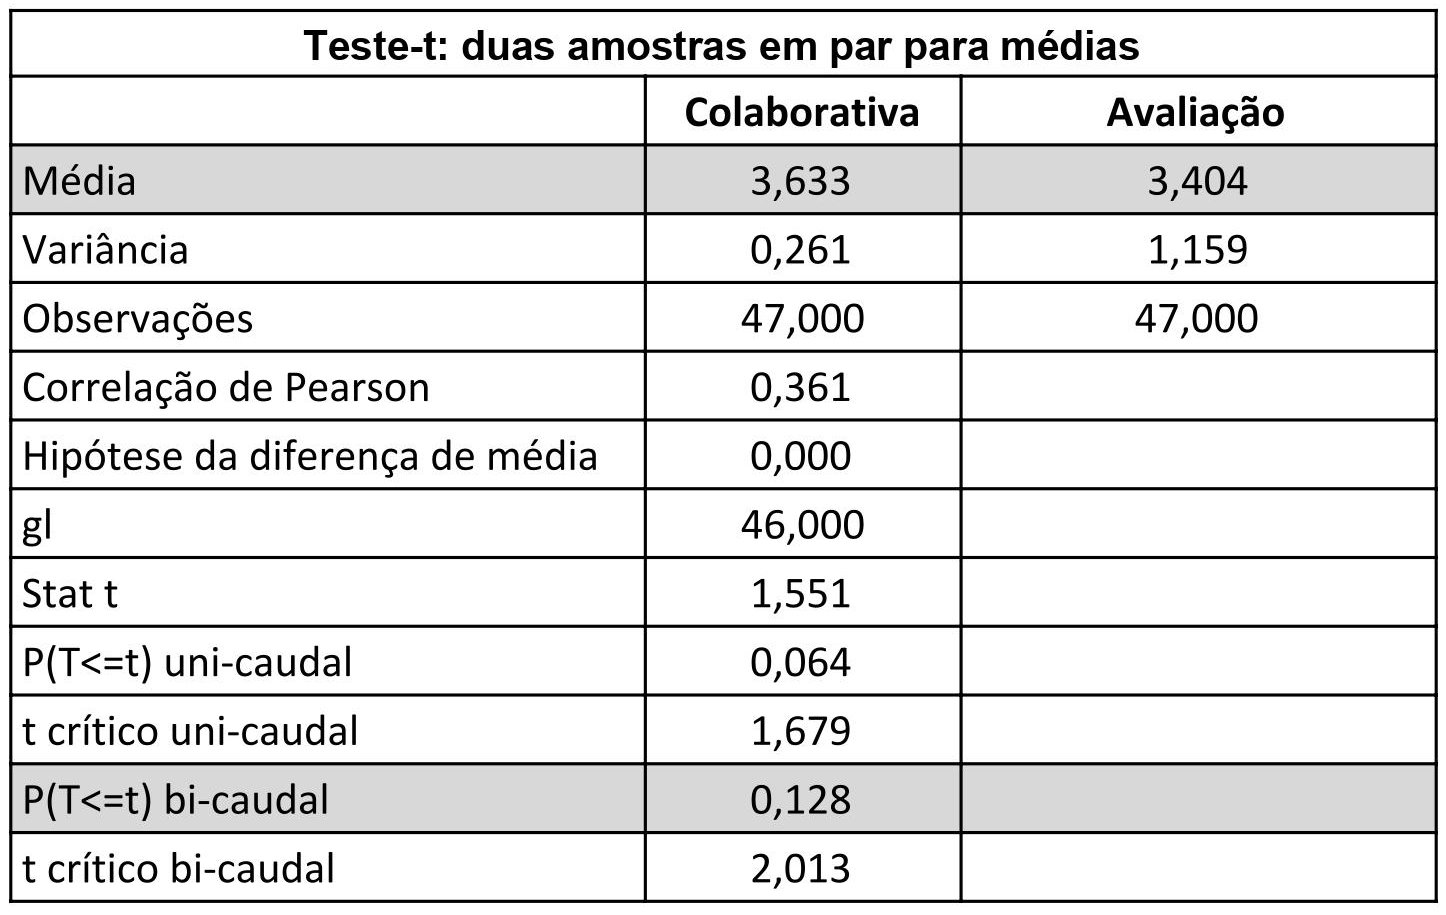
\includegraphics[width=.7\linewidth]{imagens/testeTColaborativa.jpg}
	\caption[Teste T: Filtragem Colaborativa]{Teste T: Filtragem Colaborativa}
    \label{fig:testeTColaborativa}
\end{figure}

A partir dos resultados obtidos na figura \ref{fig:testeTColaborativa}, pode-se observar que o valor de \textbf{P(t<=t) bi-caudal} é superior a \textbf{0,05}. Isso significa que as recomendações para filtragem colaborativa foram boas, uma vez que são iguais estatisticamente as avaliações dos usuários.

\begin{figure}[H]
	\centering
	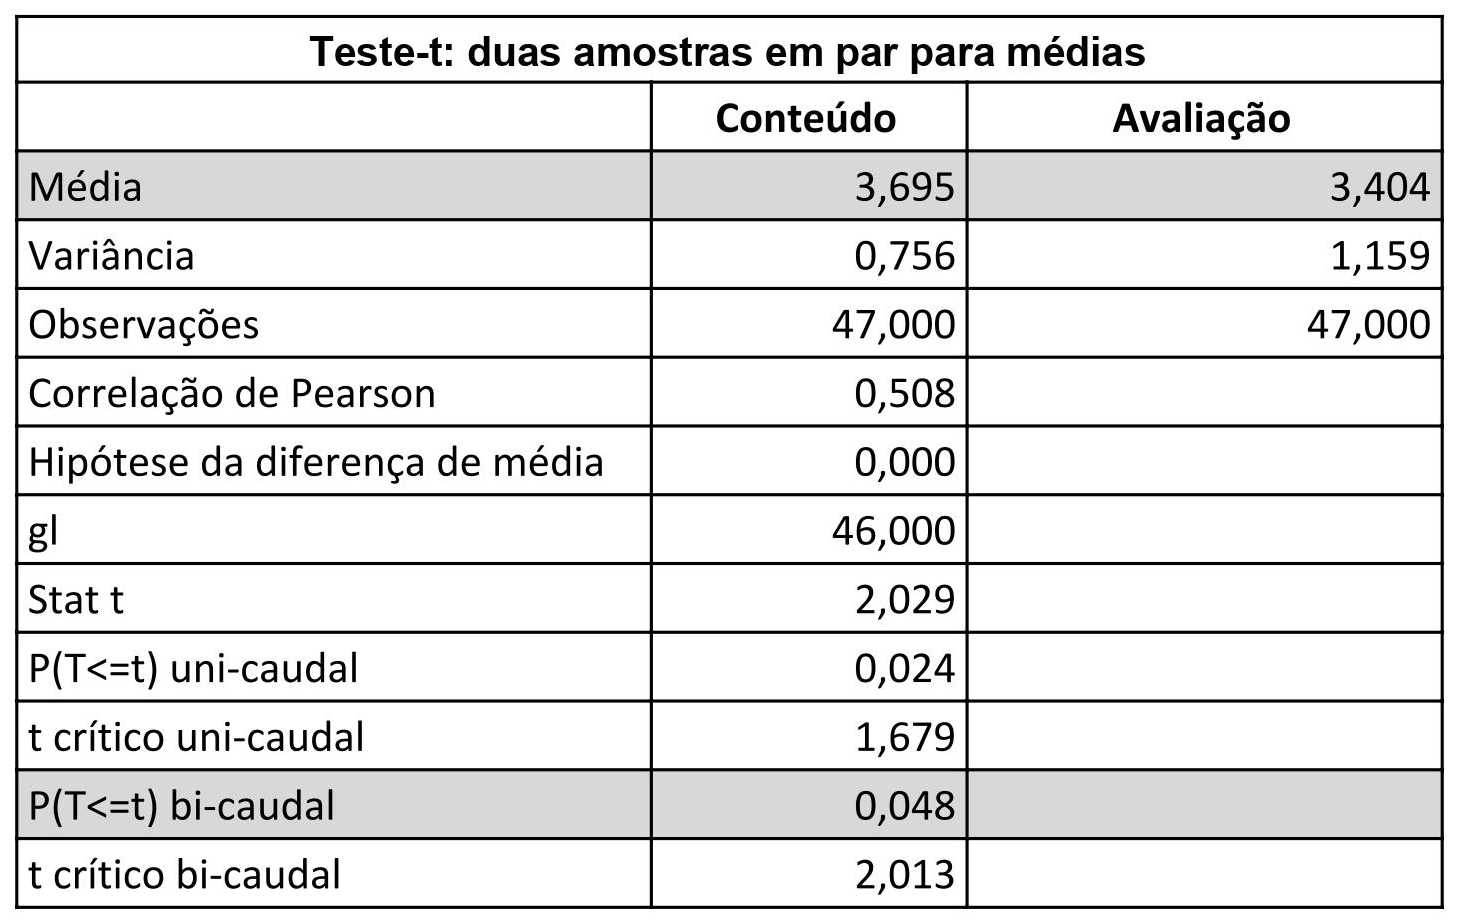
\includegraphics[width=.7\linewidth]{imagens/testeTConteudo.jpg}
	\caption[Teste T: Filtragem Baseada em Conteúdo]{Teste T: Filtragem Baseada em Conteúdo}
    \label{fig:testeTConteudo}
\end{figure}

Os resultados para filtragem baseada em conteúdo, apresentados na figura \ref{fig:testeTConteudo} demonstram um valor para \textbf{P(t<=t) bi-caudal} inferior a \textbf{0,05}. Com isso, é observado que existem uma divergência entre os resultados das recomendações baseadas em conteúdo se comparado com as avaliações dos usuários.

\begin{figure}[H]
	\centering
	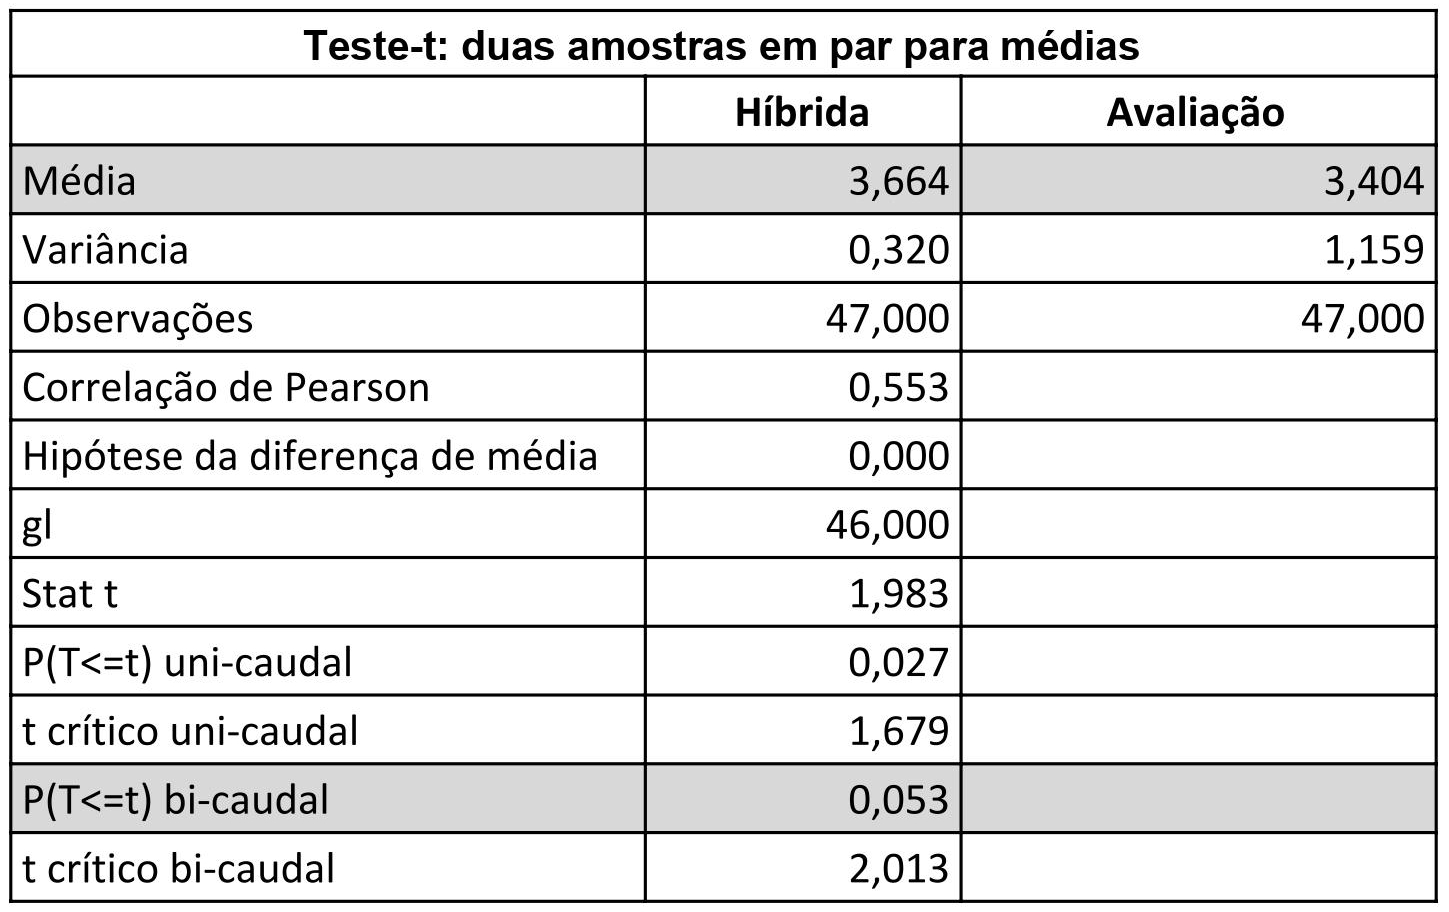
\includegraphics[width=.7\linewidth]{imagens/testeTPonderada.jpg}
	\caption[Teste T: Filtragem Híbrida Ponderada]{Filtragem Híbrida Ponderada}
    \label{fig:testeTPonderado}
\end{figure}

A partir das informações mostradas na figura \ref{fig:testeTPonderado}, é possível analisar que o valor \textbf{P(t<=t) bi-caudal} é superior a \textbf{0,05}. Isso demonstra que as recomendações geradas na filtragem híbrida ponderada são estatisticamente iguais as avaliações dos usuários.

\begin{figure}[H]
	\centering
	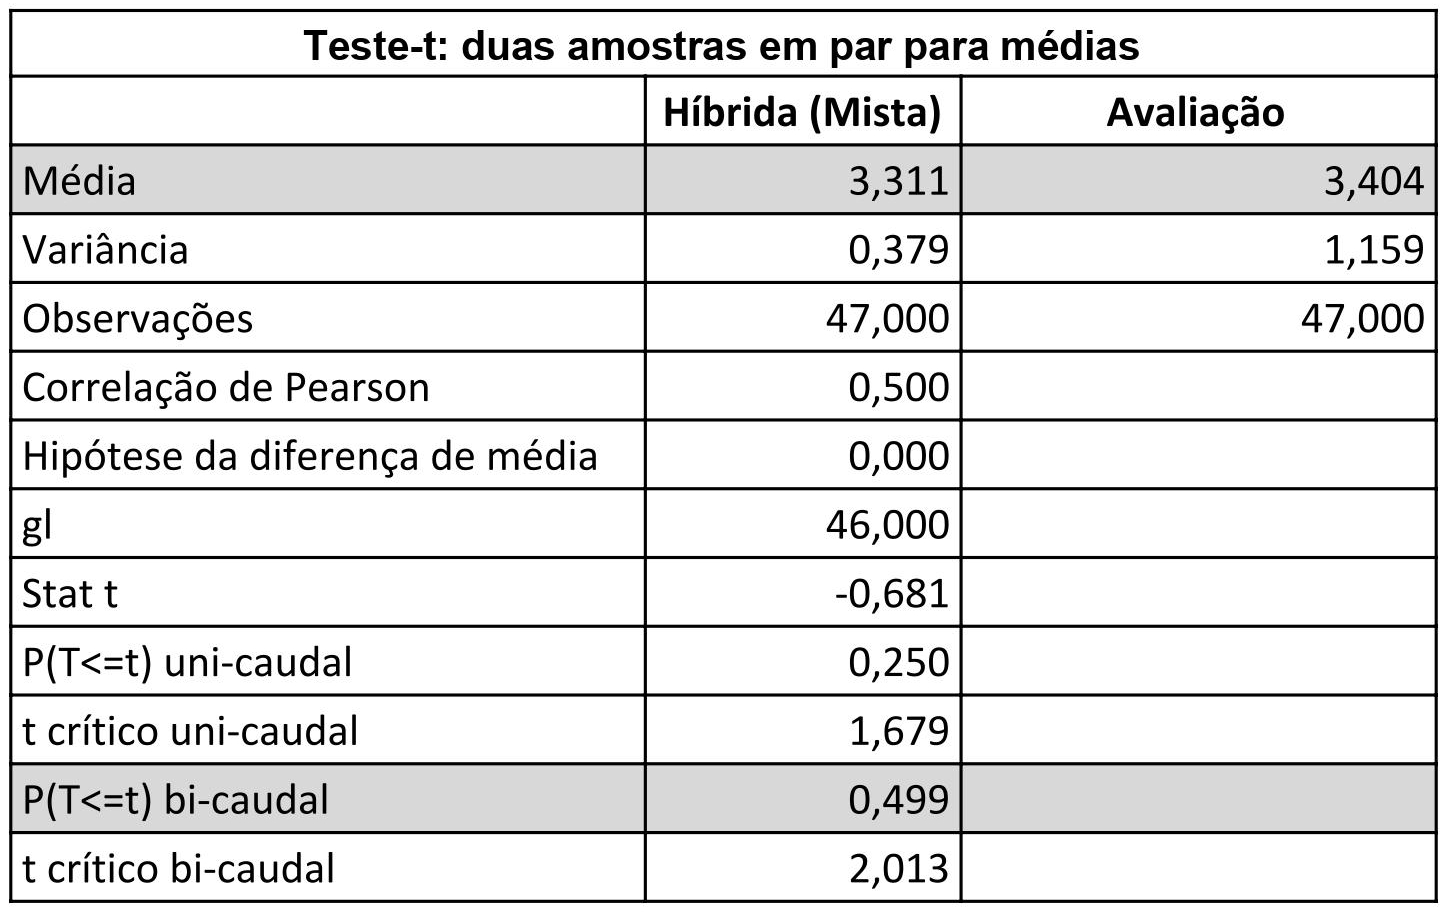
\includegraphics[width=.7\linewidth]{imagens/testeTMisto.jpg}
	\caption[Teste T: Filtragem Híbrida Mista]{Filtragem Híbrida Mista}
    \label{fig:testeTMisto}
\end{figure}

Os resultados da filtragem híbrida mista, apresentados na figura \ref{fig:testeTMisto} demonstram que o valor \textbf{P(t<=t) bi-caudal} é superior a \textbf{0,05}. Desse modo, é possível observar que os resultados apresentados pela filtragem híbrida mista são estatisticamente iguais as avaliações dos usuários.

\subsection{Resumo dos resultados}

A partir de todos os resultados apresentados, é possível definir os seguintes dados, apresentados na figura \ref{fig:resumoEstatisticaEducacional}:

\begin{figure}[H]
	\centering
	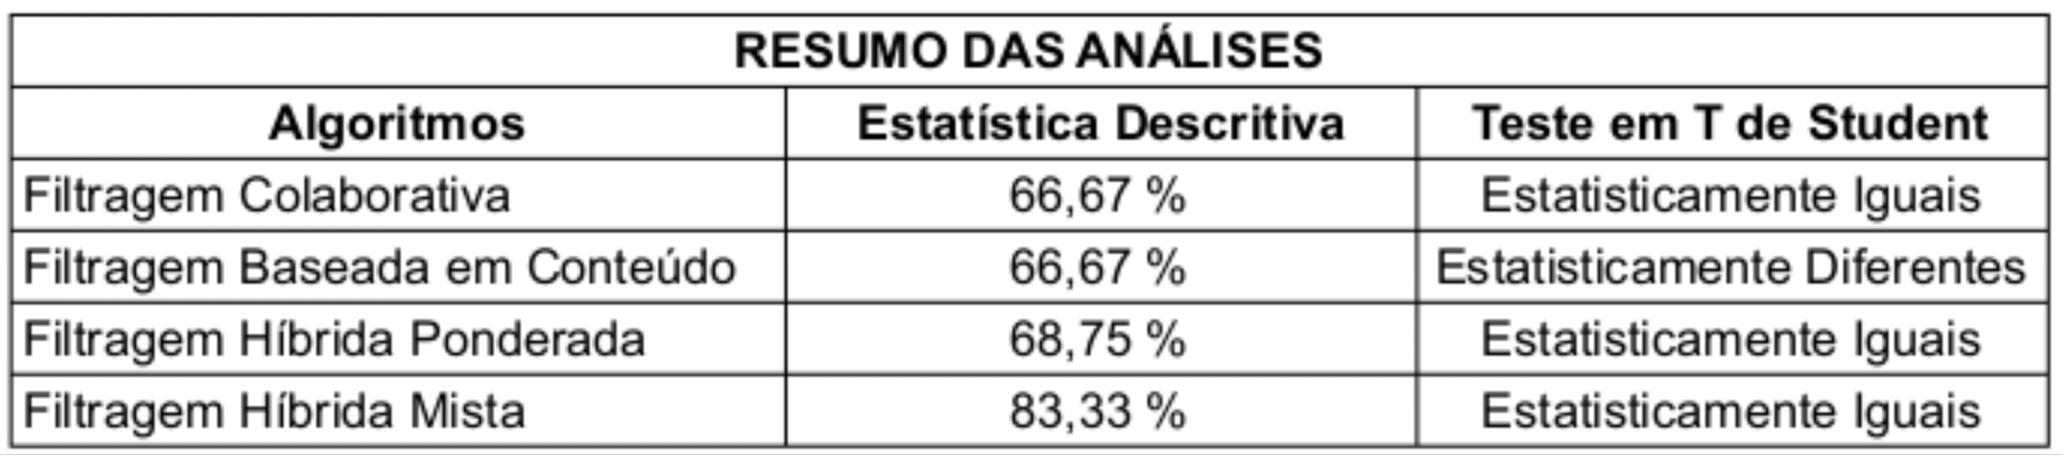
\includegraphics[width=.8\linewidth]{imagens/resumoEstatisticaEducacional.jpg}
	\caption[Resumo da estatística para o estudo de caso educacional]{Resumo da estatística para o estudo de caso educacional}
    \label{fig:resumoEstatisticaEducacional}
\end{figure}

\section{Estudo de Caso Cultural: Recomendação de Músicas}

\subsection{Contexto}

No estudo de caso realizado foi avaliado o gosto musical de diversas pessoas acerca de 10 músicas previamente selecionadas, compondo um repertório bastante variado, permitindo a definição de diversas Tags para recomendação.

Para a elaboração desse estudo foi desenvolvida uma aplicação web contextualizada para o ambiente musical, como apresentado nas figuras \ref{fig:findmusicLogin}, \ref{fig:findmusicInicio} e \ref{fig:findmusicAvaliacao}. Essa aplicação foi disponibilizada e divulgada na internet, possibilitando o acesso das pessoas que tivessem interesse.

\begin{figure}[H]
	\centering
	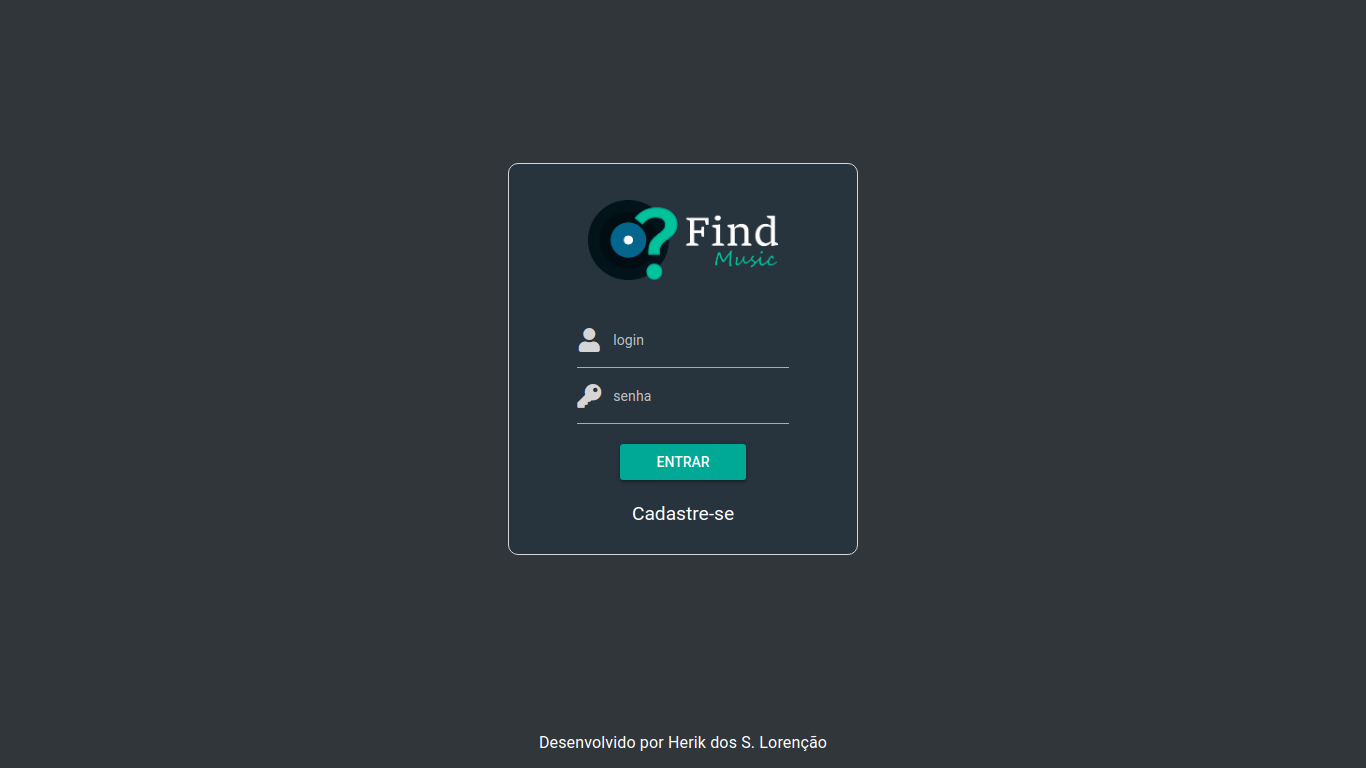
\includegraphics[width=.7\linewidth]{imagens/findmusicLogin.png}
	\caption[Aplicação cliente: Tela de Login]{Aplicação cliente: Tela de Login}
    \label{fig:findmusicLogin}
\end{figure}

\begin{figure}[H]
	\centering
	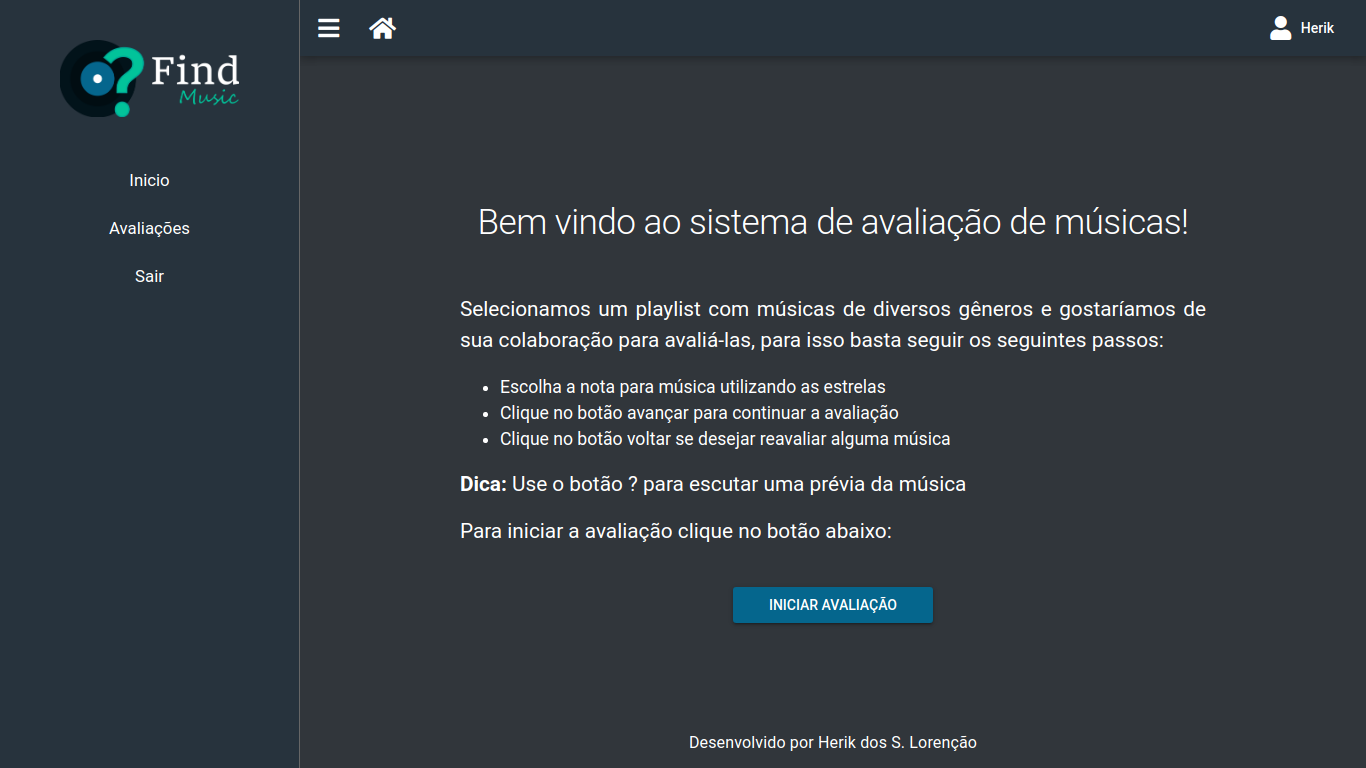
\includegraphics[width=.7\linewidth]{imagens/findmusicInicio.png}
	\caption[Aplicação cliente: Tela Inicial]{Aplicação cliente: Tela Inicial}
    \label{fig:findmusicInicio}
\end{figure}

\begin{figure}[H]
	\centering
	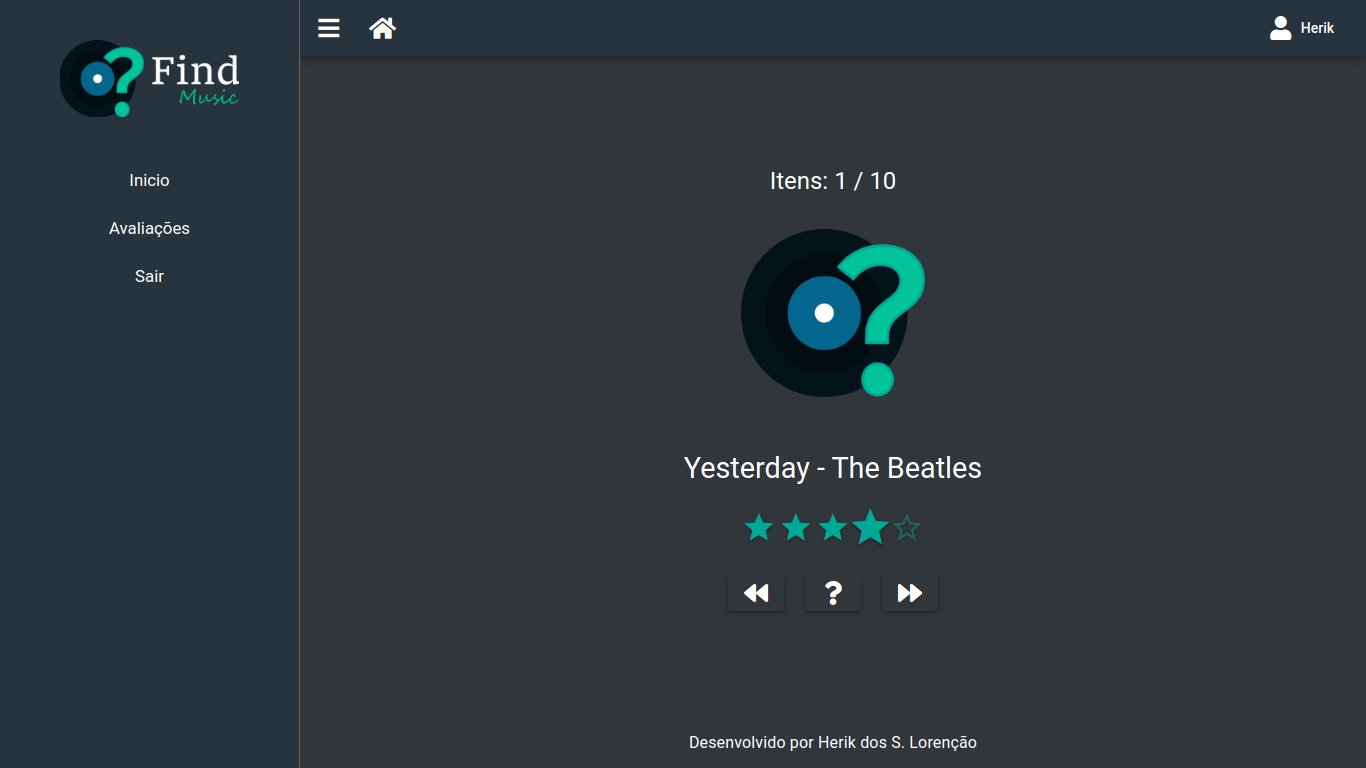
\includegraphics[width=.7\linewidth]{imagens/findmusicAvaliacao.png}
	\caption[Aplicação cliente: Avaliação]{Aplicação cliente: Avaliação}
    \label{fig:findmusicAvaliacao}
\end{figure}

A partir das avaliações recebidas foram selecionados, de forma e quantidade aleatória, valores para serem retirados das avaliações de cada avaliador, com isso, foi possível realizar o processo de recomendação e comparar o resultado recomendado com o avaliado pelo usuário. Com isso, foi possível obter os dados apresentados na tabela \ref{tableref:dadosEstudoCasoCultural}:

\begin{table}[H]
\centering
\begin{tabular}{|c|c|}
\hline
\textbf{Itens}          & \textbf{Quantidade} \\ \hline
Número de avaliadores   & 60                  \\ \hline
Número de músicas       & 10                  \\ \hline
Número de avaliações    & 600                 \\ \hline
Número de tags          & 6                   \\ \hline
Número de recomendações & 141                  \\ \hline
\end{tabular}
\caption{Dados estudo de caso cultural}
\label{tableref:dadosEstudoCasoCultural}
\end{table}

\subsection{Análise Descritiva}

Utilizando-se da análise descritiva foi possível definir a taxa de acerto do sistema sobre as recomendações que seriam aceitas pelos usuários. Nas figuras \ref{fig:findMusicEstatistica1}, \ref{fig:findMusicEstatistica2}, \ref{fig:findMusicEstatistica3} e \ref{fig:findMusicEstatistica4} pode ser observado a comparação entre as notas geradas pelas estratégias de recomendação e a nota real informada pelo usuário, o que possibilita a realização do processo de estatística descritiva.

\begin{figure}[H]
	\centering
	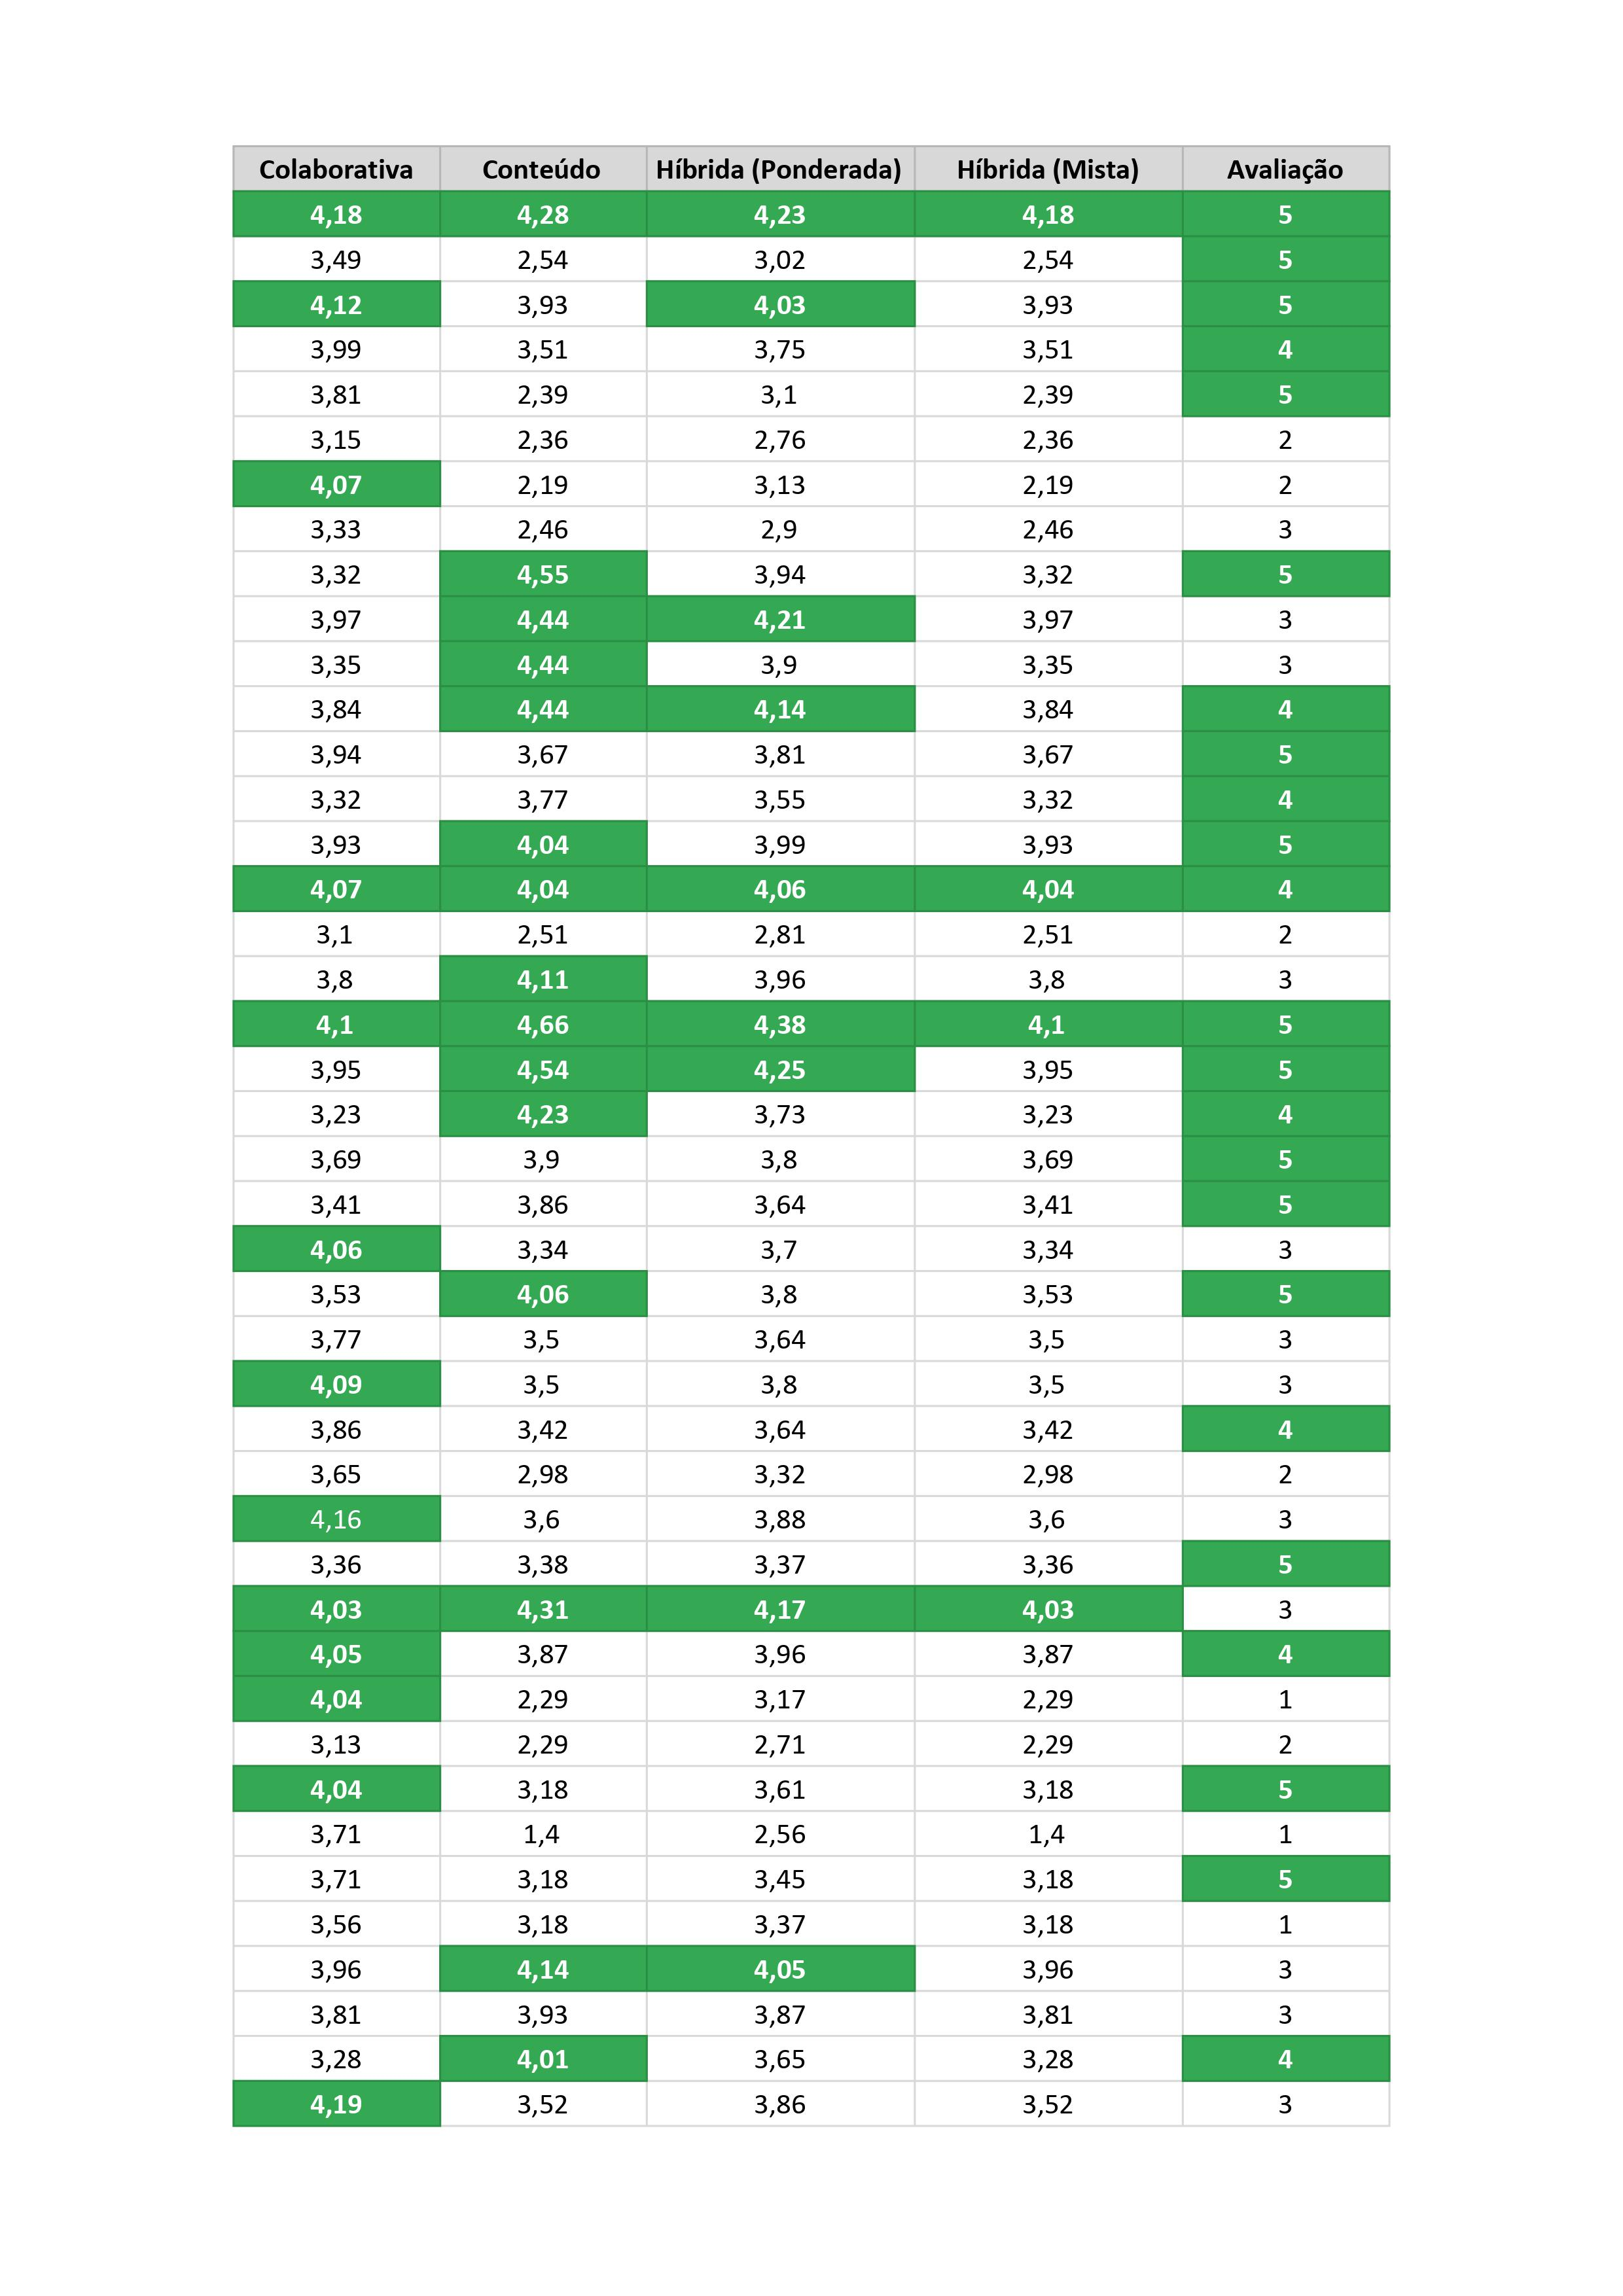
\includegraphics[width=.8\linewidth]{imagens/findMusicResultados1.jpg}
	\caption[Estatística Descritiva: Parte 1]{Estatística Descritiva: Parte 1}
    \label{fig:findMusicEstatistica1}
\end{figure}

\begin{figure}[H]
	\centering
	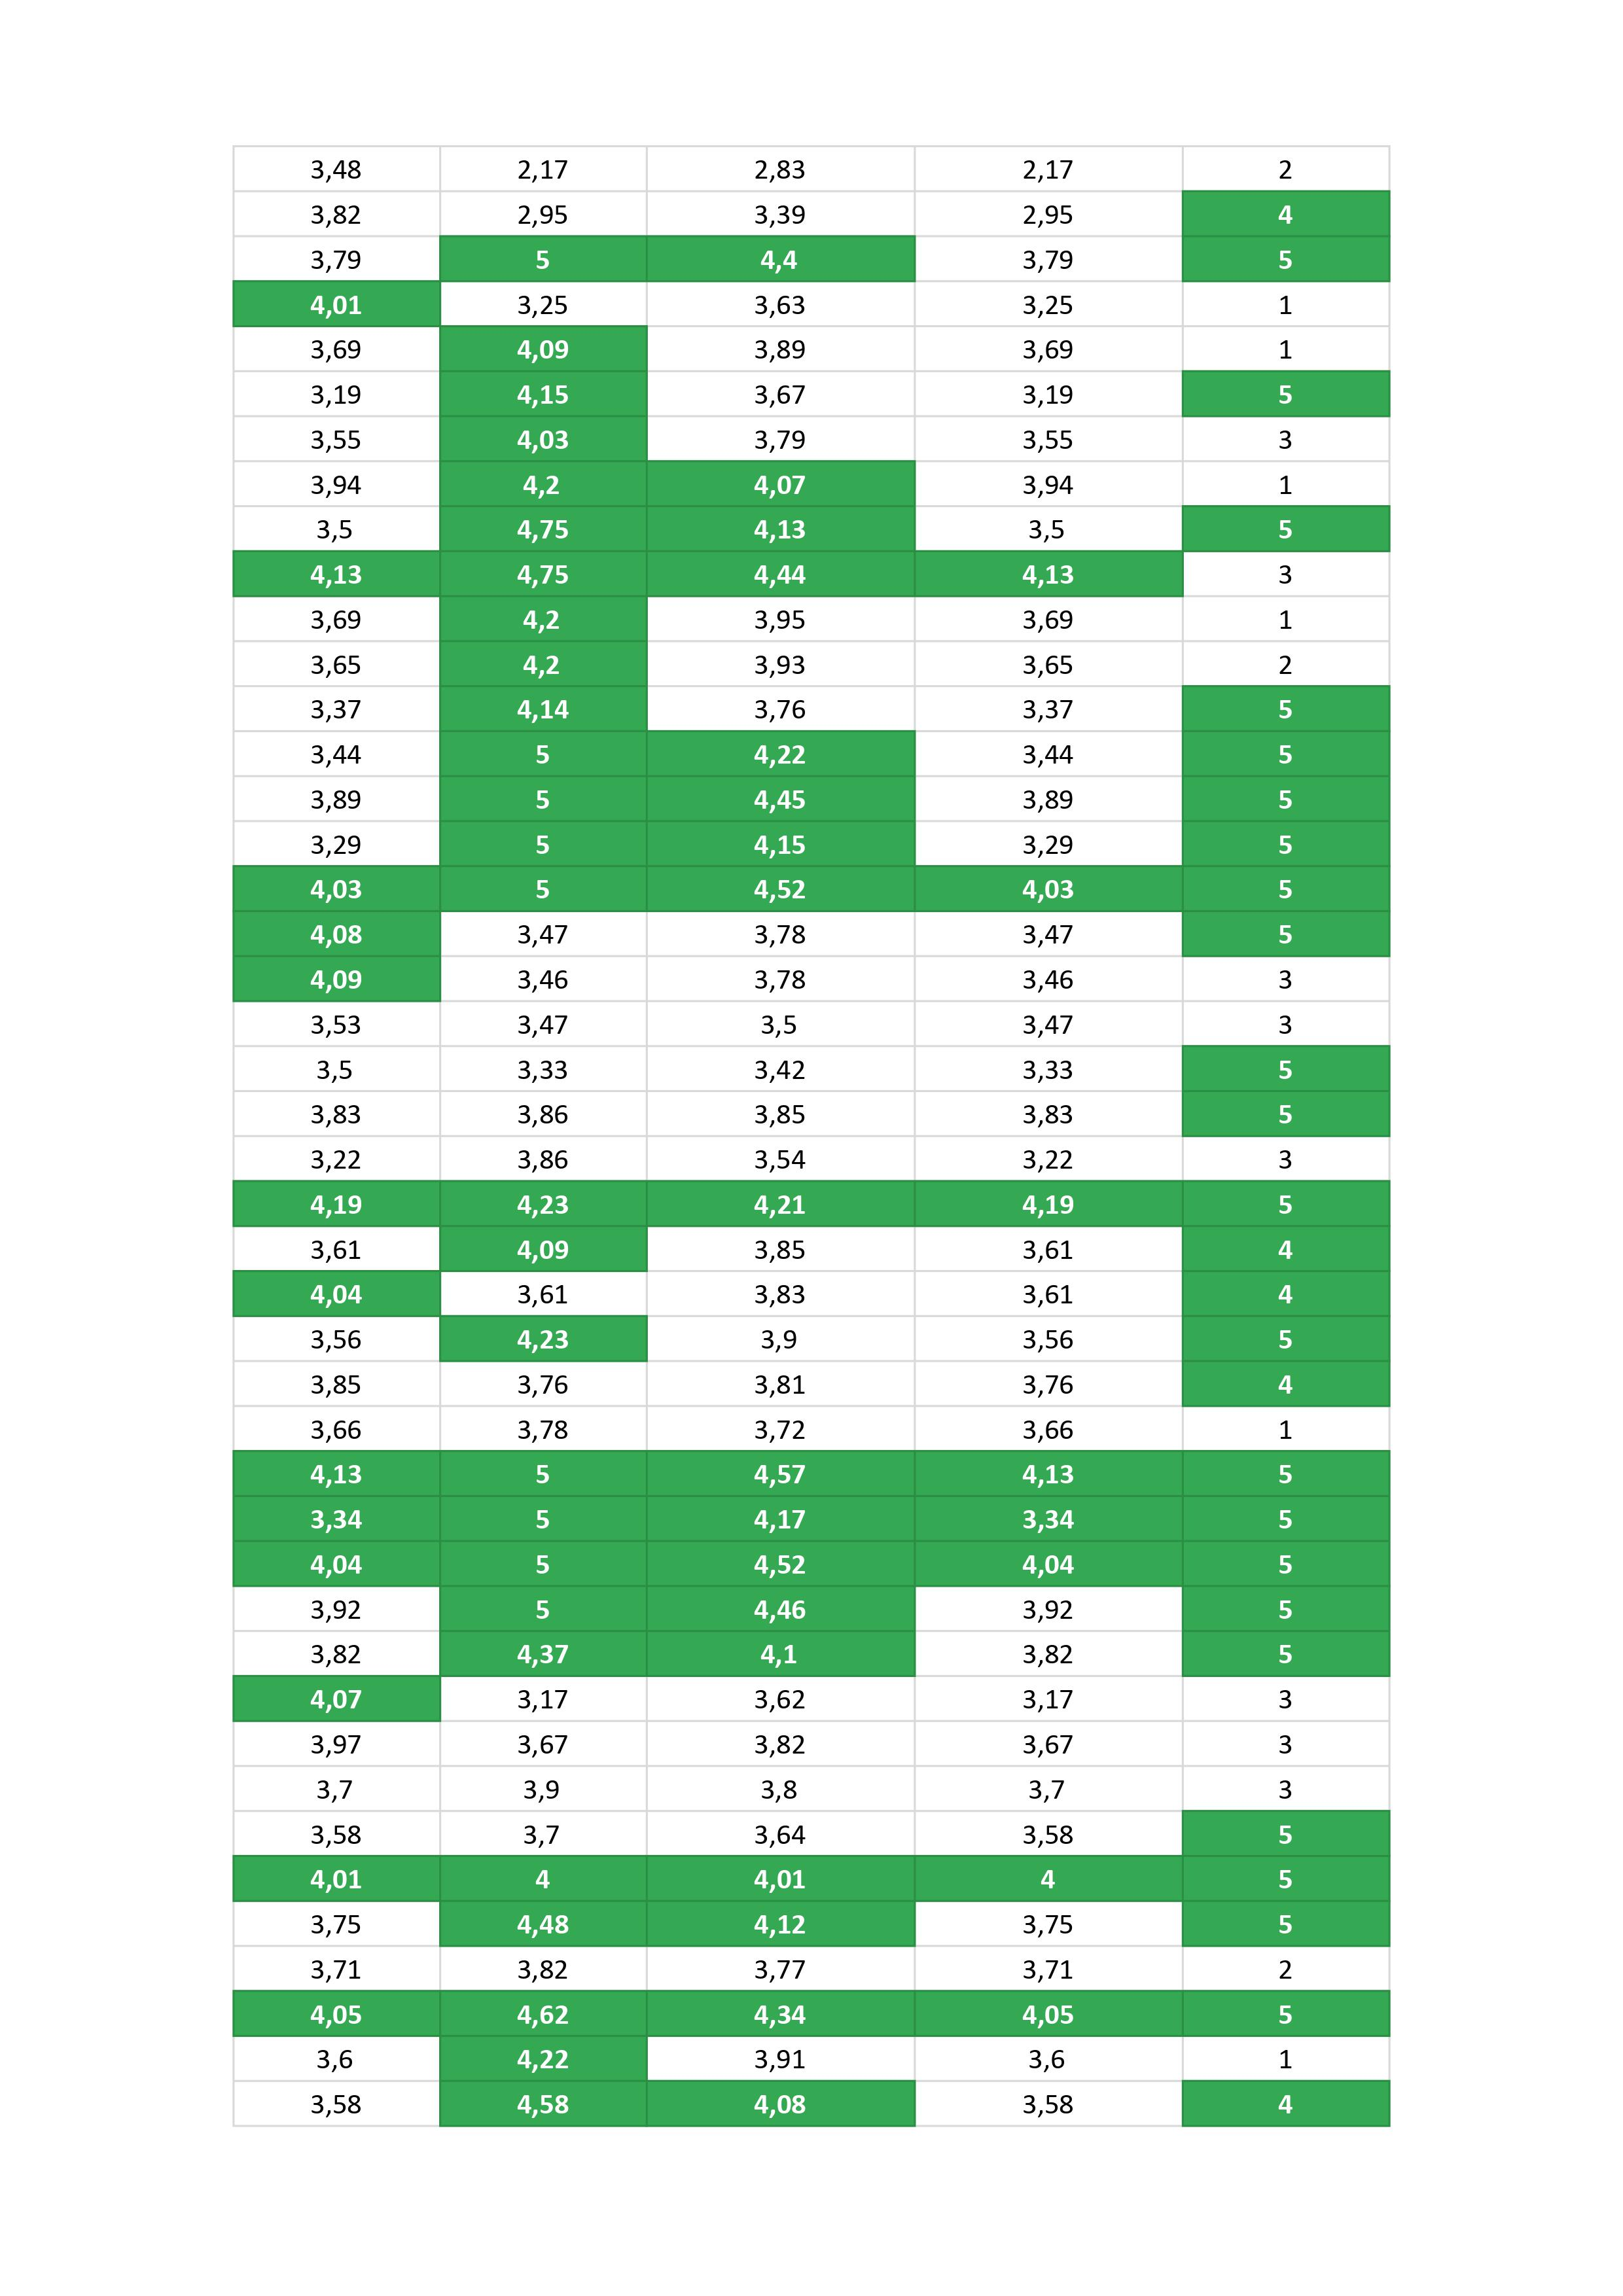
\includegraphics[width=1\linewidth]{imagens/findMusicResultados2.jpg}
	\caption[Estatística Descritiva: Parte 2]{Estatística Descritiva: Parte 2}
    \label{fig:findMusicEstatistica2}
\end{figure}

\begin{figure}[H]
	\centering
	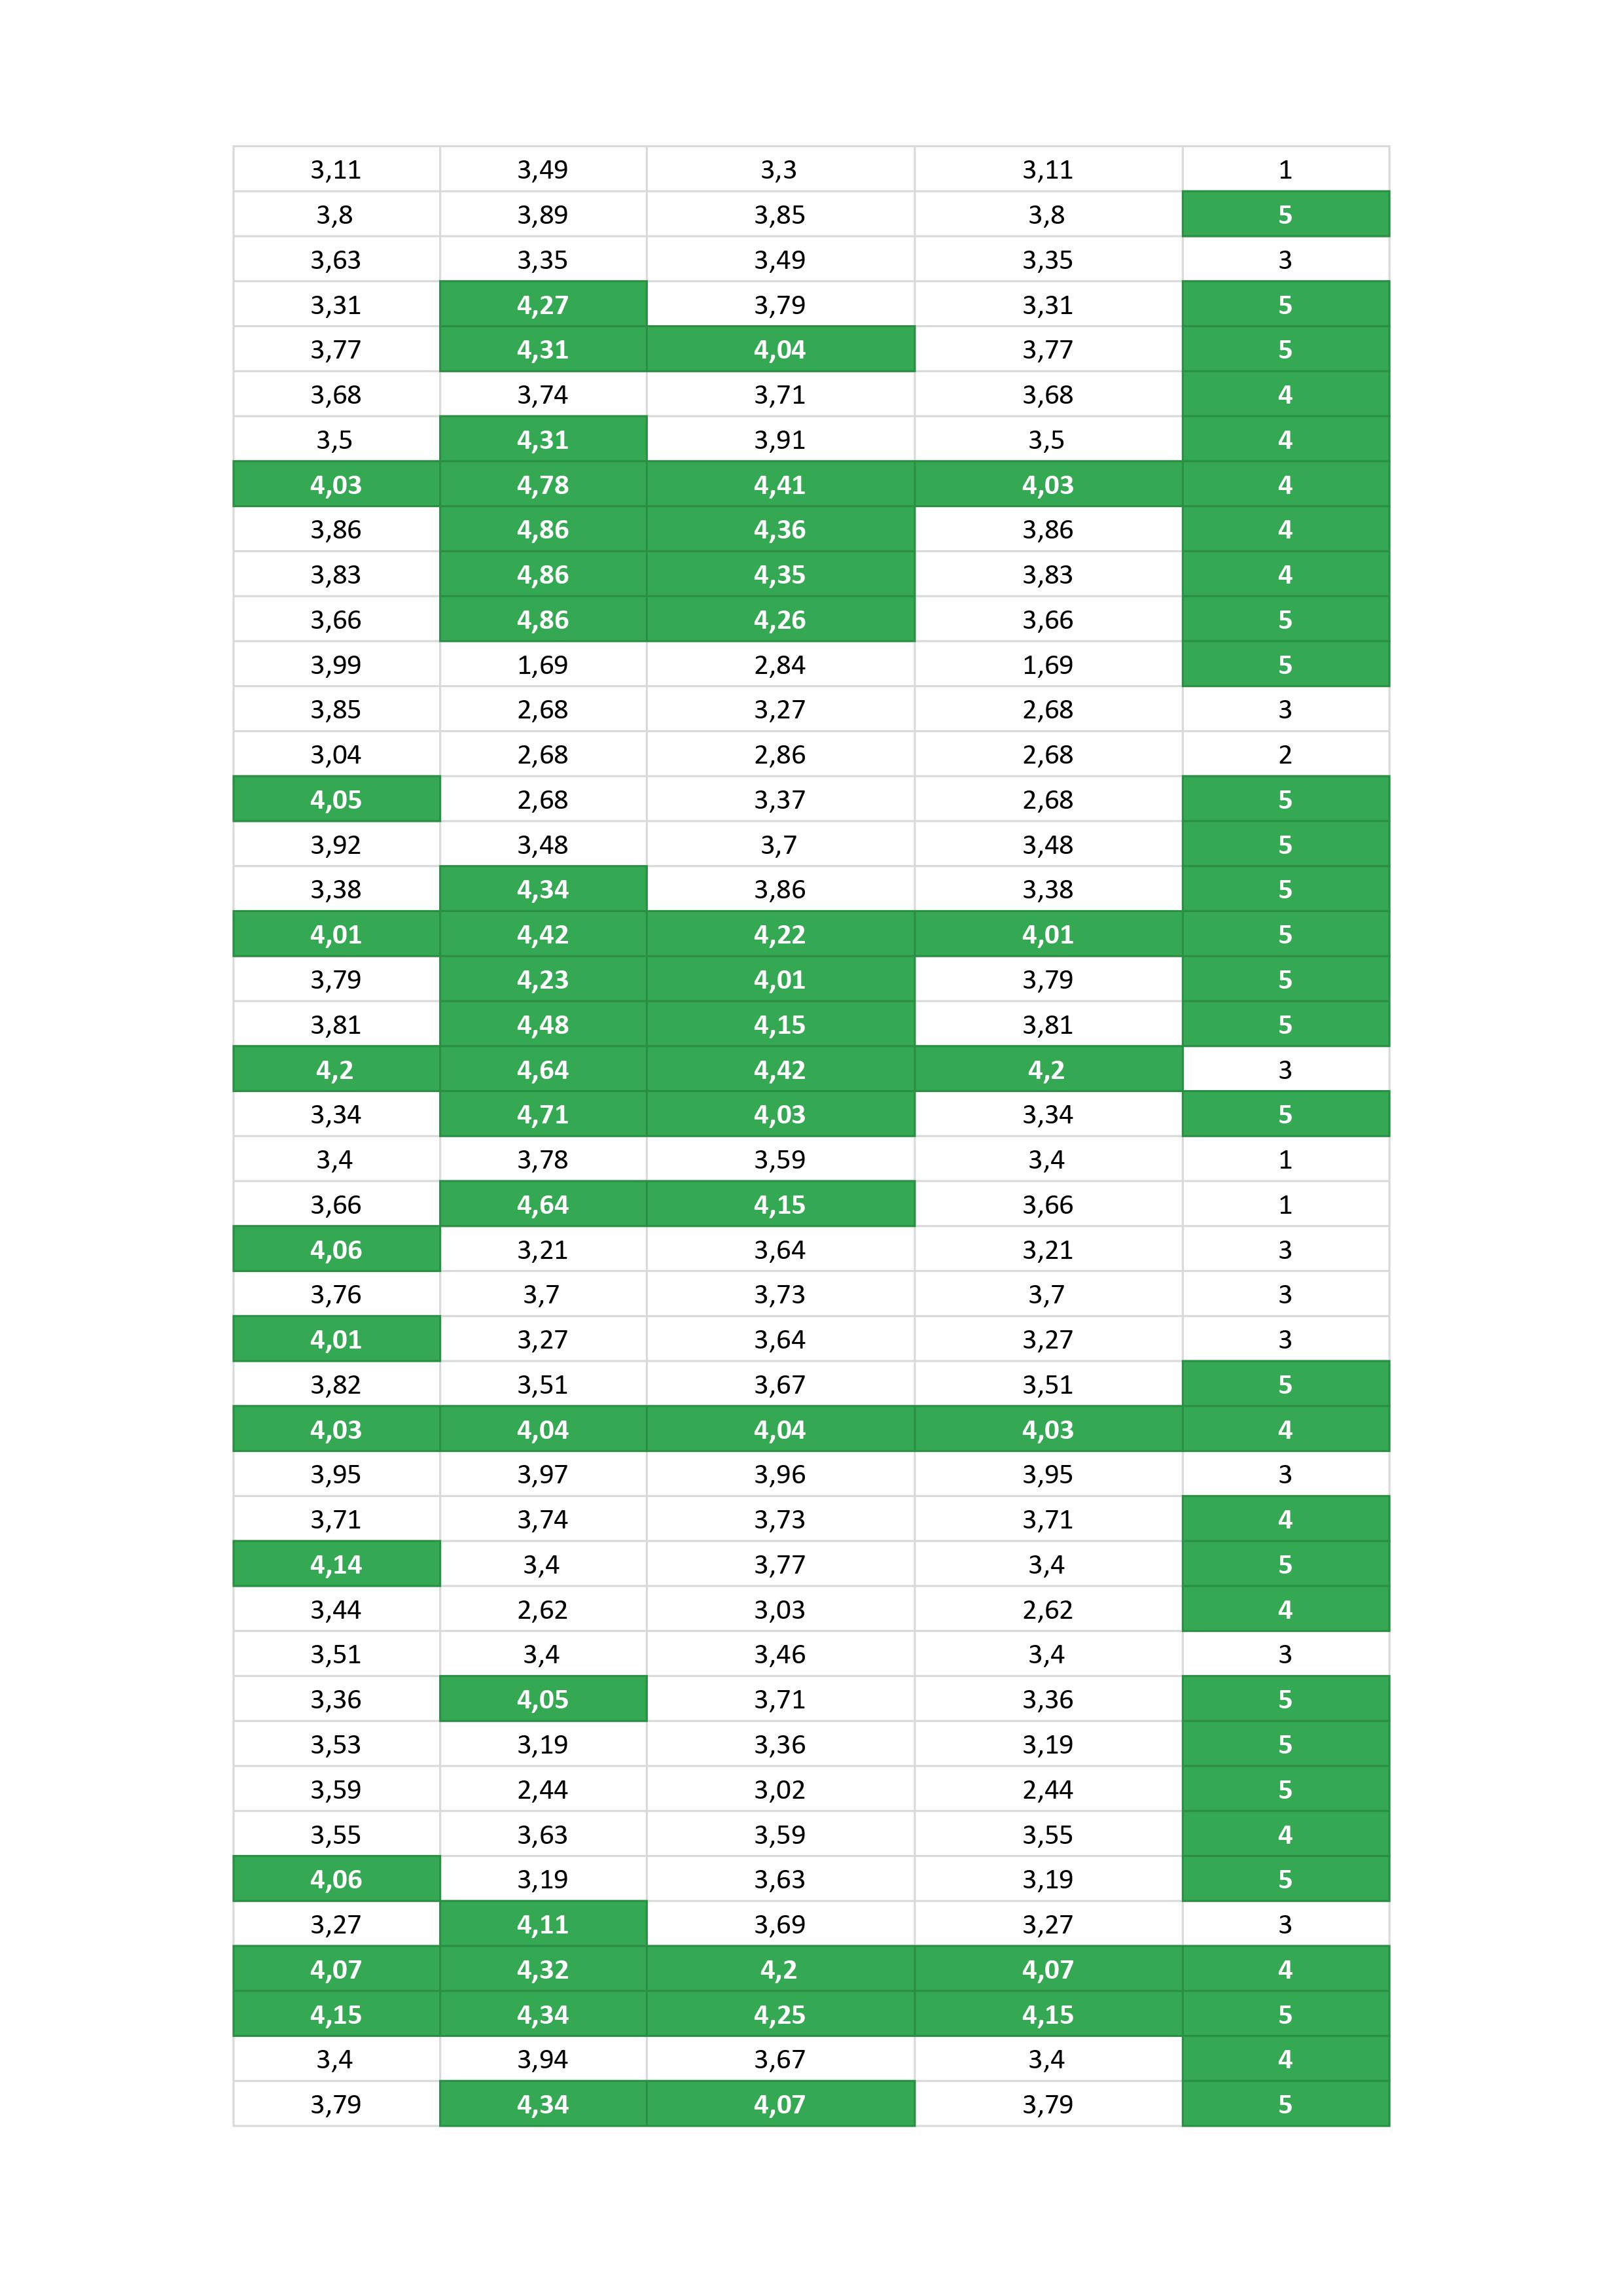
\includegraphics[width=1\linewidth]{imagens/findMusicResultados3.jpg}
	\caption[Estatística Descritiva: Parte 3]{Estatística Descritiva: Parte 3}
    \label{fig:findMusicEstatistica3}
\end{figure}

\begin{figure}[H]
	\centering
	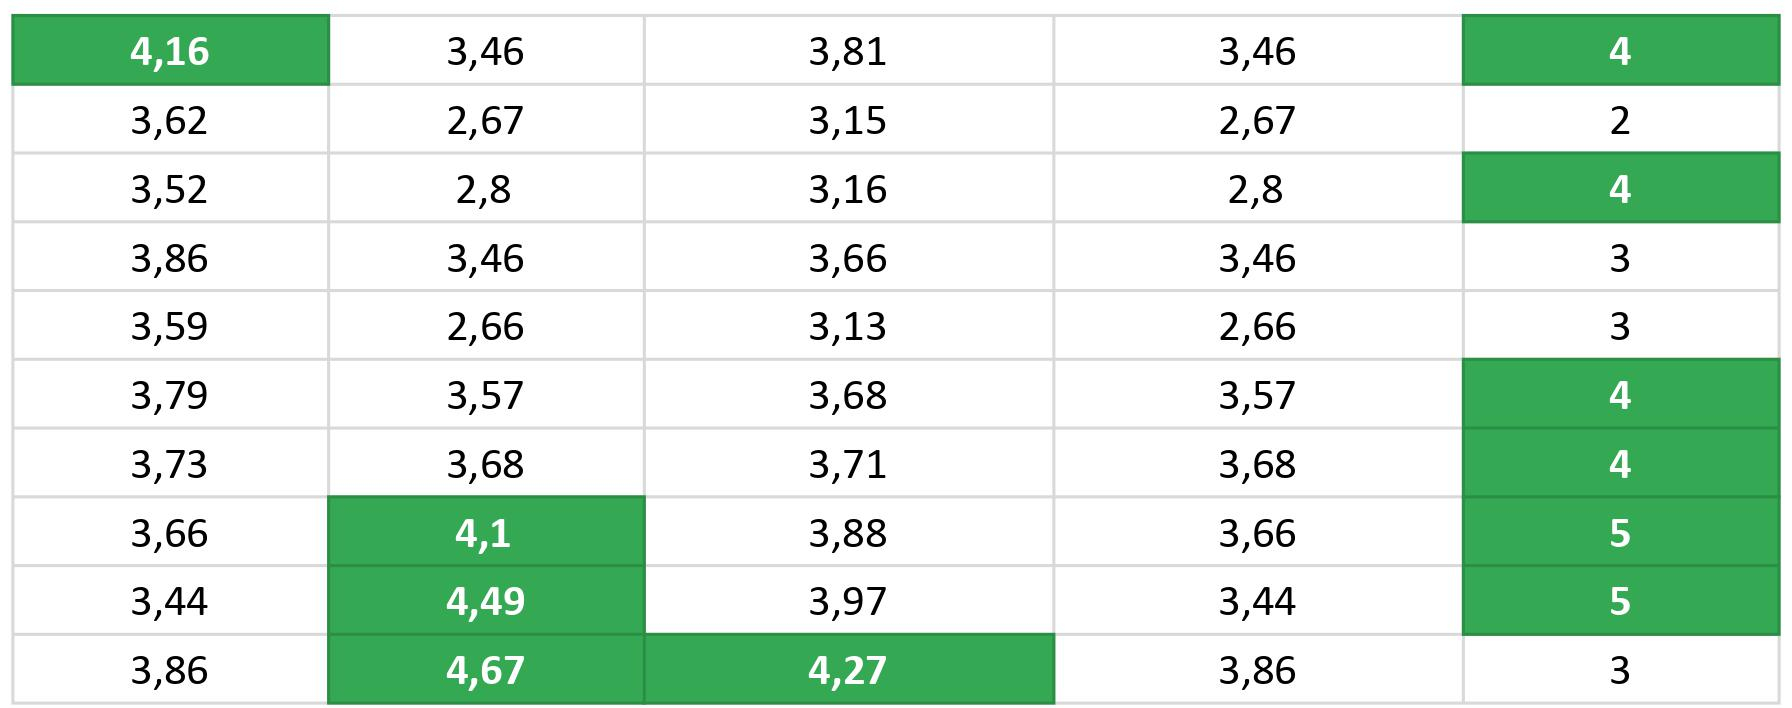
\includegraphics[width=.8\linewidth]{imagens/findMusicResultados4.jpg}
	\caption[Estatística Descritiva: Parte 4]{Estatística Descritiva: Parte 4}
    \label{fig:findMusicEstatistica4}
\end{figure}

A partir das células marcadas com a cor verde nas figuras \ref{fig:findMusicEstatistica1}, \ref{fig:findMusicEstatistica2}, \ref{fig:findMusicEstatistica3} e \ref{fig:findMusicEstatistica4}, torna-se possível observar quais itens seriam recomendados pelo sistema (tendo como consideração um ponto de corte definido como 4 pontos). Na figura \ref{fig:findMusicEstatisticaTaxa} são apresentados os resultados relativos a taxa de erros e acertos das recomendações nesse estudo de caso:

\begin{figure}[H]
	\centering
	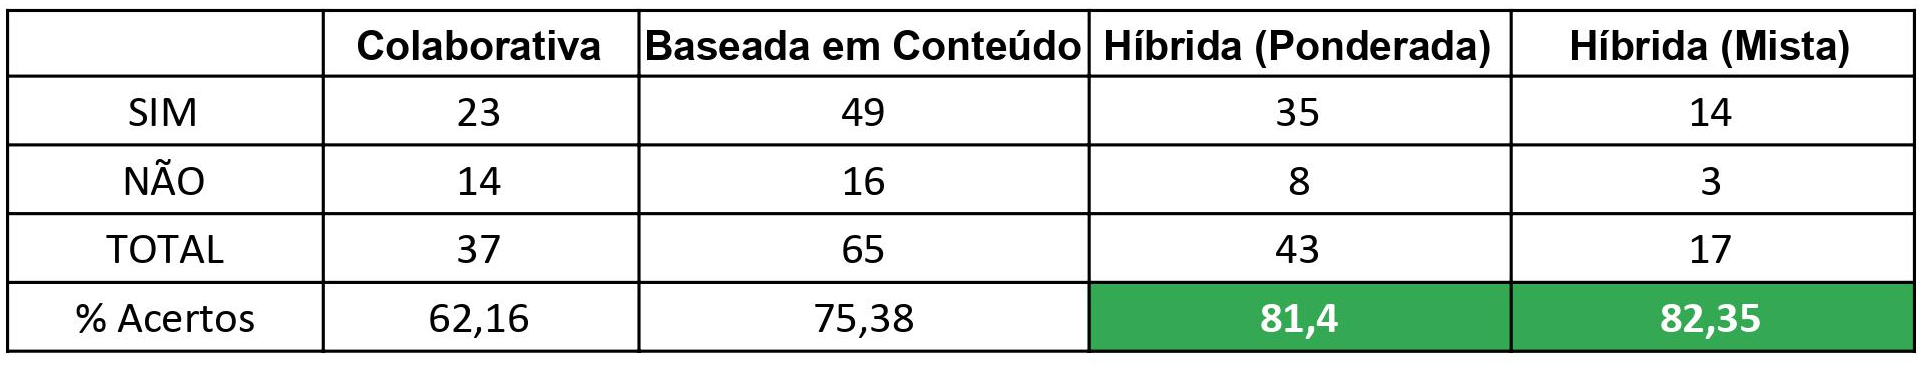
\includegraphics[width=.9\linewidth]{imagens/findmusicEstatisticaTaxa.jpg}
	\caption[Taxas da Estatística Descritiva]{Taxas da Estatística Descritiva}
    \label{fig:findMusicEstatisticaTaxa}
\end{figure}

De acordo com os dados disponíveis na figura \ref{fig:findMusicEstatisticaTaxa}, conclui-se que as abordagens híbridas (marcadas pela cor verde) obtiveram um resultado superior as estratégias colaborativa e baseada em conteúdo quando utilizadas de maneira isolada.

\subsection{Teste T de Student}

Como outra forma de avaliação estatística das recomendações foi utilizado o Teste t de Student, que busca avaliar a distância entre os resultados recomendados e as notas avaliadas em determinado item pelo avaliador. Nesse tipo de abordagem é analisado a diferença entre os valores recomendados e os avaliados pelos avaliadores, buscando a menor divergência possível entre os valores.

\begin{figure}[H]
	\centering
	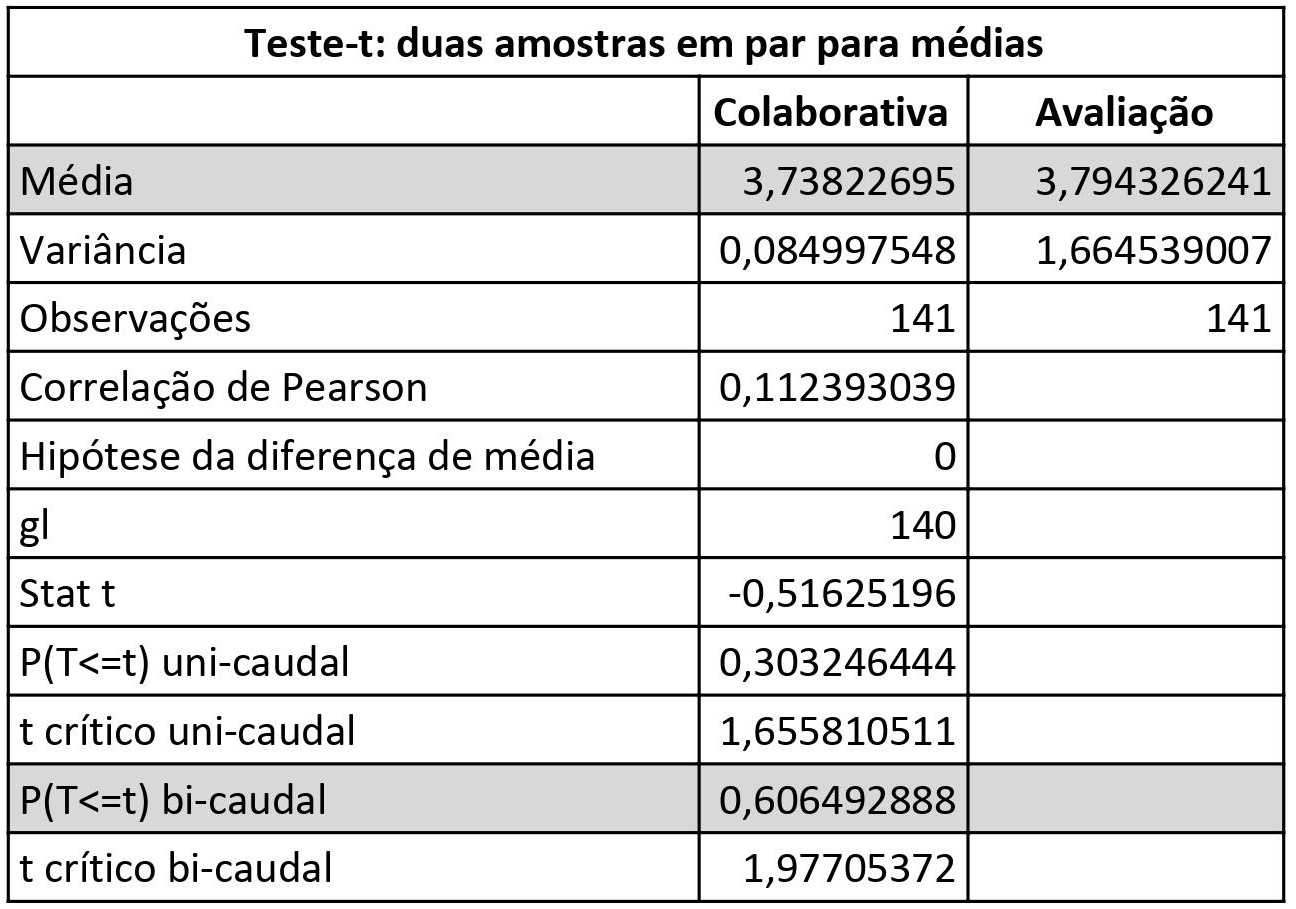
\includegraphics[width=.6\linewidth]{imagens/findmusicTesteTColaborativa.jpg}
	\caption[Teste T: Filtragem Colaborativa]{Teste T: Filtragem Colaborativa}
    \label{fig:findMusicTesteTColaborativa}
\end{figure}

Com os resultados obtidos na figura \ref{fig:findMusicTesteTColaborativa}, pode-se observar que o valor de \textbf{P(t<=t) bi-caudal} é superior a \textbf{0,05}. Desse modo, é possível definir que as recomendações para filtragem colaborativa foram boas, uma vez que são estatisticamente iguais as avaliações dos usuários.

\begin{figure}[H]
	\centering
	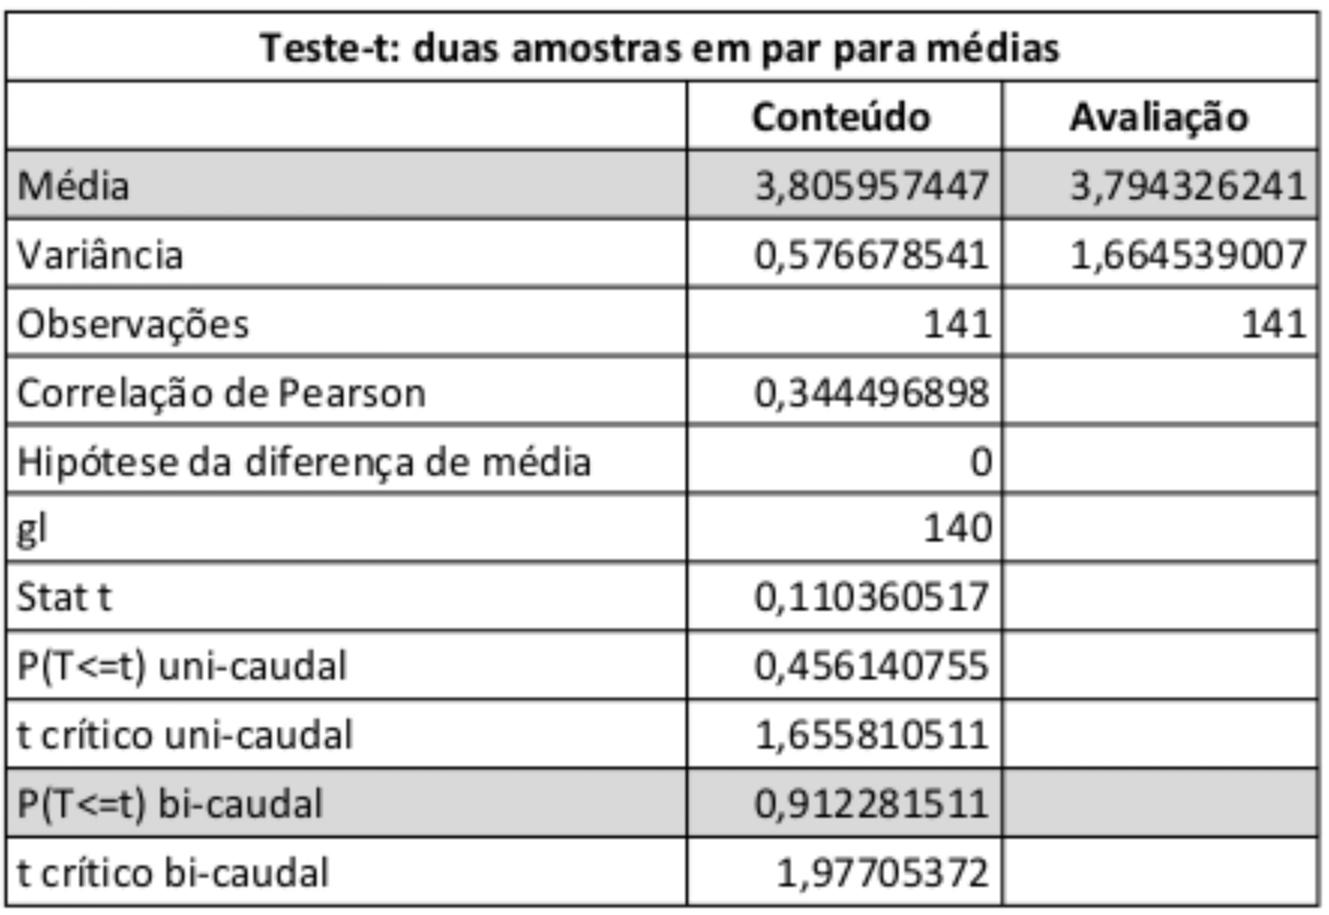
\includegraphics[width=.6\linewidth]{imagens/findmusicTesteTConteudo.jpg}
	\caption[Teste T: Filtragem Baseada em Conteúdo]{Teste T: Filtragem Baseada em Conteúdo}
    \label{fig:findMusicTesteTConteudo}
\end{figure}

Com os dados obtidos na figura \ref{fig:findMusicTesteTConteudo}, é visto que o valor \textbf{P(t<=t) bi-caudal} é superior a \textbf{0,05}. Esse resultado permite definir que as recomendações geradas na filtragem baseada em conteúdo são estatisticamente iguais as avaliações dos usuários.

\begin{figure}[H]
	\centering
	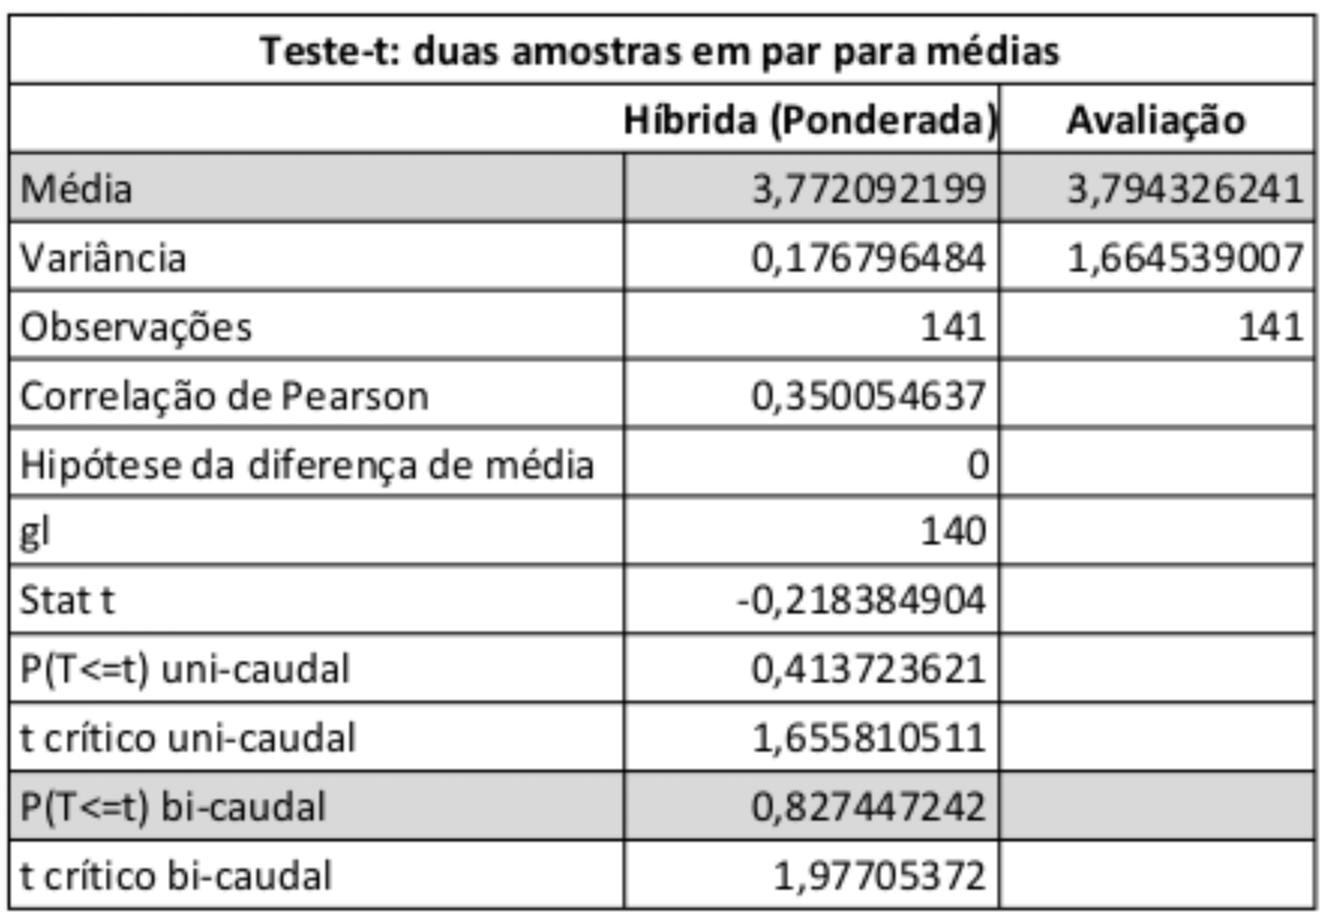
\includegraphics[width=.6\linewidth]{imagens/findmusicTesteTPonderado.jpg}
	\caption[Teste T: Filtragem Híbrida Ponderada]{Teste T: Filtragem Híbrida Ponderada}
    \label{fig:findMusicTesteTPonderado}
\end{figure}

Com os dados definidos na figura \ref{fig:findMusicTesteTPonderado}, é possível observar que o valor \textbf{P(t<=t) bi-caudal} superior a \textbf{0,05}. Isso demonstra que as recomendações da filtragem híbrida ponderada são estatisticamente iguais as avaliações dos usuários.

\begin{figure}[H]
	\centering
	\includegraphics[width=.6\linewidth]{imagens/findmusicTesteTMista.jpg}
	\caption[Teste T: Filtragem Híbrida Mista]{Filtragem Híbrida Mista}
    \label{fig:findMusicTesteTMista}
\end{figure}

De acordo com a figura \ref{fig:findMusicTesteTMista}, os resultados das recomendações da abordagem híbrida mista não apresentam bons níveis de similaridade com as avaliações dos usuários, visto que, o valor \textbf{P(t<=t) bi-caudal} é inferior a \textbf{0,05}.

\subsection{Resumo dos resultados}

Como resumo dos resultados gerados acima, é possível definir os seguintes dados, apresentados na figura \ref{fig:resumoEstatisticaCultural}:

\begin{figure}[H]
	\centering
	\includegraphics[width=.8\linewidth]{imagens/resumoEstatisticaCultural.jpg}
	\caption[Resumo da estatística para o estudo de caso cultural]{Resumo da estatística para o estudo de caso cultural}
    \label{fig:resumoEstatisticaCultural}
\end{figure}
\chapter{\textbf{Conclusão}} % Este comando é utilizado para criar capítulos

\section{Análise Geral do Trabalho}

O trabalho desenvolvido propiciou o desenvolvimento de um sistema de recomendação híbrido, prosseguindo com os estudos desenvolvidos nos trabalhos de \citeonline{tccluisa} e \citeonline{tcctiago}.

Com o desenvolvimento aberto para comunidade e disponibilização de uma API documentada, além de aplicações para visualização e geração das recomendações torna-se possível a utilização e melhoria do sistema por qualquer pessoa que possua interesse. Vale ressaltar que a estrutura do código foi desenvolvida buscando a modularização, o que acaba por possibilitar a adição de novas funcionalidades no sistema sem muito esforço.

A partir do estudo de caso aplicado, foi possível avaliar que a recomendação híbrida apresentou resultados estatisticamente superiores as abordagens colaborativa e baseada em conteúdo quando utilizadas individualmente, demonstrando desse modo a viabilidade dessa abordagem para recomendação.

Acerca do uso da concorrência, infelizmente, não foi atingido o objetivo esperado, apresentando problemas no tempo de execução. Enquanto isso, a recomendação offline mostrou resultados satisfatórios podendo, desse modo, se apresentar como uma alternativa viável para melhoria de performance do sistema. 

\section{Trabalhos Futuros}

Como trabalhos futuros para sistema podem ser adicionados novas abordagens de recomendação, possibilitando o estudo e aplicação de novas técnicas. Novos sistemas de consulta e visualização de dados também podem ser desenvolvidos buscando atingir nichos ou plataformas diferentes.

Com o estudo mais profundo da área de arquitetura e desenvolvimento de sistemas distribuídos pode ser que a técnica de concorrência apresente-se como uma solução mais viável, podendo ser desenvolvida com sucesso em novos trabalhos.
%%% ====================================================================
%%% Início da parte pós-textual do documento.
\postextual


%%% Referências Bibliográfica

\bibliography{bibliografia/bibliography}

%%% Início dos apêndices ---------------------------------------------
\apendices


% --------------------------------------------------------------------
\chapter{Titulo}

\begin{enumerate}
    \item Item 1
    \item Item 2
\end{enumerate}

% --------------------------------------------------------------------



%%% Início dos anexos ------------------------------------------------
\anexos

\partanexos*

\chapter{Algoritmo de recomendação}

\section{Filtragem Colaborativa}

\subsection{Estruturação dos dados}

Inicialmente é necessário organizar os dados existentes para a realização da recomendação. Para isso, é gerado um tabela que demonstra as notas avaliadas pelos avaliadores para os itens no sistema, conforme mostrado na figura \ref{fig:avaliacoes}. Os campos em amarelo representam os valores ainda não avaliados, sendo tarefa do sistema de recomendação calcular as possíveis notas dos avaliadores para esses campos.

\begin{figure}[H]
	\centering
	\includegraphics[width=0.8\linewidth]{imagens/recomendacaoAvaliacoes.jpg}
	\caption[Avaliações dos itens pelos avaliadores]{Avaliações dos itens pelos avaliadores}
    \label{fig:avaliacoes}
\end{figure}

\subsection{Similaridade entre os avaliadores}

Como a recomendação colaborativa usa como base o conceito de vizinhança para seus cálculos, é necessário medir a distância existente entre os avaliadores. Para esse exemplo será usado o cálculo da distância do avaliador Jorge em relação a todos os outros avaliadores do sistema, conforme mostrado na figura \ref{fig:similaridadeJorge}. De maneira geral, esse processo deverá ser realizado para todos os avaliadores do sistema.

\begin{figure}[H]
	\centering
	\includegraphics[width=1\linewidth]{imagens/similaridadeJorge.png}
	\caption[Cálculo da similaridade do Jorge com os avaliadores]{Cálculo da similaridade do Jorge com os avaliadores}
    \label{fig:similaridadeJorge}
\end{figure}

Para esse cálculo foi utilizado a fórmula da distância euclidiana, utilizando como parâmetros as notas informadas pelos avaliadores em cada um dos itens. Para cálculo da distância euclidiana é utilizado um conjunto de pares, representado pela notas de Jorge e do avaliador calculado no momento acerca de determinado item. Caso algum dos parâmetros esteja vazio, a coordenada é ignorada pelo algoritmo no cálculo da distância.

Para facilitar a visualização o cálculo da distância euclidiana foi decomposto nos seguintes passos:

\begin{itemize}
    \item Definição das coordenadas;
    \item Cálculo do quadrado da diferença;
    \item Somatório dos quadrados da diferença;
    \item Raiz quadrado do somatório dos quadrados da diferença.
\end{itemize}

Nos cálculos abaixo, é possível observar a geração da distância euclidiana entre Jorge e Bianca:

\subsubsection{Definição das coordenadas}

Separando as coordenadas válidas obteremos uma tabela conforme demonstrado na figura \ref{fig:coordenadasEuclidiana}:

\begin{figure}[H]
	\centering
	\includegraphics[width=.7\linewidth]{imagens/coordenadasEuclidiana.jpg}
	\caption[Coordenadas para distância euclidiana]{Coordenadas para distância euclidiana entre Jorge e Bianca}
    \label{fig:coordenadasEuclidiana}
\end{figure}

\subsubsection{Cálculo do quadrado da diferença}

Aplicando a fórmula do quadrado da diferença nas coordenadas apresentadas na figura \ref{fig:coordenadasEuclidiana} é possível chegar nos resultados descritos na figura \ref{fig:quadradoDiferenca}:

\begin{equation*}
    {F(x,y) = \left( x_{i}-y_{i}\right)^2 }
    \label{eq:quadradoDiferenca}
\end{equation*}

\begin{figure}[H]
	\centering
	\includegraphics[width=.8\linewidth]{imagens/quadradoDiferenca.jpg}
	\caption[Quadrado da diferença das coordenadas]{Quadrado da diferença das coordenadas}
    \label{fig:quadradoDiferenca}
\end{figure}

\subsubsection{Somatório dos quadrados da diferença}

Nessa etapa, somente é necessário realizar a soma entre os dados encontrados na função \textbf{F(x)} mostrada na figura \ref{fig:quadradoDiferenca}. Desse modo chega-se na seguinte equação \ref{eq:somaQuadrados}:

\begin{equation*}
    \begin{aligned}
    {S(x,y)& = 0.25 + 12.25 + 2.25} \\
    {S(x,y)& = 14.75}
    \end{aligned}
    \label{eq:somaQuadrados}
\end{equation*}

\subsubsection{Raiz quadrado do somatório dos quadrados da diferença}

Aplicando a raiz quadrado sobre o resultado do somatório obtido na equação \ref{eq:somaQuadrados} obtemos o seguinte resultado apresentado na equação \ref{eq:raizSomaQuadrados}:

\begin{equation*}
    \begin{aligned}
    {D(x,y)& = \sqrt{S(x, y)} \\
    {D(x,y)& = \sqrt{14.75}} \\
    {D(x,y)& \approx{3.84}
    \end{aligned}
    \label{eq:raizSomaQuadrados}
\end{equation*}

A partir desses resultados é possível obter um coeficiente de distância entre o usuário Jorge e Bianca de aproximadamente \textbf{3.84}. A partir desse valor, é possível realizar a análise de distância entre todos os usuários do sistema e definir os vizinhos, que seriam os que apresentarem menor coeficiente de distância.

Para facilitar a visualização da distância também pode ser definido um coeficiente de similaridade, que poderia ser representado com a equação \ref{eq:similaridade} mostrada abaixo:

\begin{equation*}
    \begin{aligned}
    {Sm(x,y)& = 1/(1 + D(x,y))} \\
    {Sm(x,y)& = 1/1 + 3.84}} \\
    {Sm(x,y)& \approx{0.21}
    \end{aligned}
    \label{eq:similaridade}
\end{equation*}

Com o coeficiente de similaridade definido, podemos visualizar que quando maior esse valor, maior será a proximidade entre os usuários.

\subsection{Similaridade entre itens}

Com os coeficientes de similaridade definidos, pode-se analisar calcular as notas dos itens para recomendação. Na abordagem colaborativa a similaridade dos usuários será utilizada como forma de peso para as suas avaliações, sendo que quanto mais próximo os usuários estejam, maior será o impacto de suas avaliações na nota que será recomendada pelo sistema.

Levando a análise do Jorge como exemplo, pode-se calcular as notas avaliadas pelos outros usuários acerca dos itens. Para isso, é realizado a multiplicação entre as notas avaliadas e o coeficiente de similaridade entre Jorge e o usuário em questão, conforme mostrado na figura \ref{fig:similaridadeAvaliacoes}:

\begin{figure}[H]
	\centering
	\includegraphics[width=1\linewidth]{imagens/similaridadeAvaliacao.PNG}
	\caption[Similaridade x Avaliações]{Similaridade x Avaliações}
    \label{fig:similaridadeAvaliacoes}
\end{figure}

\subsection{Cálculo da recomendação}

Com os dados de similaridade de itens disponíveis, é possível calcular a possível nota que o usuário dará para os itens que ainda não avaliou. Utilizando o exemplo do Jorge, é possível visualizar que a bateria ainda não foi avaliada. Dessa forma, pode-se calcular essa nota, utilizando os seguintes passos descritos abaixo:

\begin{itemize}
    \item Soma das similaridades dos usuários;
    \item Soma das similaridades dos itens;
    \item Cálculo da recomendação.
\end{itemize}

\subsubsection{Soma das similaridades dos usuários}

Para realização dessa conta basta selecionar todos os usuários que avaliaram o item que será recomendado (no exemplo do Jorge, a bateria) e somar o valor de suas similaridades, conforme a equação \ref{eq:somatorioSimilaridadeUsuarios}:

\begin{equation*}
    \begin{aligned}
    {Su(x,y)& = 0.21}
    \end{aligned}
    \label{eq:somatorioSimilaridadeUsuarios}
\end{equation*}

\textbf{OBS:} Como Carlos não avaliou a bateria sua nota será desconsiderada nesse cálculo.

\subsubsection{Soma das similaridades dos itens}

Nessa etapa. deve-se realizar o somatório de todos as avaliações do item que será recomendado. No exemplo utilizado, usaremos somente a nota da Bianca acerca da bateria, uma vez que o Carlos não avaliou esse item. Com isso, chegamos na equação \ref{eq:somatorioSimilaridadeUsuarios}:

\begin{equation*}
    \begin{aligned}
    {Si(x,y)& = 0.8}
    \end{aligned}
    \label{eq:somatorioSimilaridadeUsuarios}
\end{equation*}

\subsubsection{Cálculo da recomendação}

Com os somatórios das similaridades realizados, basta realizar uma divisão entre seus valores, conforme mostrado na equação \ref{eq:calculoRecomendacaoColaborativa} para se obter o valor da recomendação do item.

\begin{equation*}
    \begin{aligned}
    {R(x,y)& = Si/Su} \\
    {R(x,y)& = 0.8/0.21}
    {R(x,y)& = 3.8}
    \end{aligned}
    \label{eq:calculoRecomendacaoColaborativa}
\end{equation*}

Com isso podemos definir que a nota gerada pelo sistema para bateria ao Jorge será de \textbf{3.8}.

\section{FILTRAGEM BASEADA EM CONTEÚDO}

\subsection{Estruturação dos dados}

A organização dos dados iniciais para filtragem baseada em conteúdo pode ser dividida em duas partes, sendo uma da relação entre os avaliadores e os itens (igual a utilizada na filtragem colaborativa) e outra que apresenta os vínculos entre os itens e as tags. Ambas as tabelas podem ser visualizadas nas figuras \ref{fig:avaliacoes2} e \ref{fig:itensTags}:

\begin{figure}[H]
	\centering
	\includegraphics[width=.8\linewidth]{imagens/recomendacaoAvaliacoes.jpg}
	\caption[Avaliações dos itens pelos avaliadores]{Avaliações dos itens pelos avaliadores}
    \label{fig:avaliacoes2}
\end{figure}

\begin{figure}[H]
	\centering
	\includegraphics[width=.8\linewidth]{imagens/itemTags.PNG}
	\caption[Itens x Tags]{Itens x Tags}
    \label{fig:itensTags}
\end{figure}

\subsection{Identificação dos Perfis}

Na filtragem baseada em conteúdo têm-se como principal alvo o uso das características dos itens para geração da recomendação. Para isso, necessita-se criar e avaliar qual o impacto de cada tag para o usuário avaliado.

Para essa avaliação, será realizado a criação de perfil para o usuário. Usando o exemplo do Jorge, pode-se chegar no perfil apresentado na figura \ref{fig:perfilUsuario} a partir da multiplicação da nota avaliada pelo usuário e a relação entre item e tag existente para cada item. Vale ressaltar que nas duas últimas linhas da tabela exibida na figura \ref{fig:perfilUsuario} têm-se o somatório e média de cada tag.

\begin{figure}[H]
	\centering
	\includegraphics[width=.8\linewidth]{imagens/perfilUsuario.PNG}
	\caption[Perfil do Jorge]{Perfil do Jorge}
    \label{fig:perfilUsuario}
\end{figure}

\subsection{Similaridade entre as tags}

Para definir a similaridade dos itens com o usuário é necessário do perfil criado no passo anterior. Para definição dos coeficientes é necessário realizar o cálculo da distância euclidiana entre as notas avaliadas pelo usuário e os valores calculados para seu perfil. Para exemplificação, pode-se analisar a figura \ref{fig:coordenadasConteudo} que mostra o cálculo da distância euclidiana entre Jorge e o Celular:

\begin{figure}[H]
	\centering
	\includegraphics[width=.8\linewidth]{imagens/coordenadasConteudo.PNG}
	\caption[Coordenadas para distância euclidiana]{Coordenadas para distância euclidiana}
    \label{fig:coordenadasConteudo}
\end{figure}

Após realização dos cálculos pode-se obter o coeficiente de similaridade entre Jorge e os itens, conforme mostrado na figura \ref{fig:similaridadeConteudo}. Vale ressaltar que os cálculos de distância euclidiana e coeficiente de similaridade são os mesmos apresentados na seção de filtragem colaborativa, apenas mudando as variáveis comparadas. 

\begin{figure}[H]
	\centering
	\includegraphics[width=1\linewidth]{imagens/similaridadeConteudo.PNG}
	\caption[Similaridade de Itens com Jorge]{Similaridade de Itens com Jorge}
    \label{fig:similaridadeConteudo}
\end{figure}

\subsection{Similaridade entre os itens}

A partir da realização dos passos anteriores, é possível definir a similaridade dos itens multiplicando seu perfil com o valor de similaridade obtido na etapa anterior. Desse modo, é possível chegar no resultado mostrado na figura \ref{fig:similaridadeConteudoItem}:

\begin{figure}[H]
	\centering
	\includegraphics[width=1\linewidth]{imagens/similaridadeConteudoItem.PNG}
	\caption[Similaridade dos Itens com as tags]{Similaridade dos Itens com as tags}
    \label{fig:similaridadeConteudoItem}
\end{figure}

\subsection{Cálculo da nota das tags do Item}

Com a similaridade dos itens definida, é possível definir o peso das característica para os itens ainda não avaliados. Para isso, é necessário a realização dos seguintes passos:

\begin{itemize}
    \item Somatório das similaridades da tag avaliada;
    \item Somatório das similaridades dos itens que possuem a tag avaliada;
    \item Divisão dos somatórios das similaridades.
\end{itemize}

\subsubsection{Somatório das similaridades da tag avaliada}

Utilizando como base a tabela exibida na figura \ref{fig:similaridadeConteudoItem} pode-se exemplificar o somatório da tag \textbf{Musical}. Para isso, basta realizar o somatório da columa \textbf{Sim. x Mus}, como mostrado na equação abaixo:

\begin{equation*}
    \begin{aligned}
    {St(x,y)& = 0 + 2.23 + 0 + 2.23} \\
    {St(x,y)& = 4.46}
    \end{aligned}
    \label{eq:calculoRecomendacaoColaborativa}
\end{equation*}

\subsubsection{Somatório das similaridades dos itens que possuem a tag avaliada}

Para realização desse cálculo é necessário selecionar todos os itens tem vínculo com a tag analisada e realizar o somatório de sua similaridade. No exemplo será utilizada a tag \textbf{Musical}, fazendo com que sejam selecionados os itens \textbf{Guitarra} e \textbf{Fone}. O valor da similaridade está disponível no perfil do usuário e a conta realizada é mostrada na equação \ref{eq:somaSimilaridadeItem}:

\begin{equation*}
    \begin{aligned}
    {Sit(x,y)& = 0.56 + 0.64} \\
    {Sit(x,y)& = 1.2}
    \end{aligned}
    \label{eq:somaSimilaridadeItem}
\end{equation*}

\subsubsection{Divisão dos somatórios das similaridades}

Com os somatórios realizados nos itens anteriores, basta realizar o passo mostrado na equação \ref{eq:valorTagItem} para descobrir o valor da tag para o item que ainda não foi avaliado (no exemplo usado, a bateria).

\begin{equation*}
    \begin{aligned}
    {Vt(x,y)& = St(x,y)/Sit(x,y)} \\
    {Vt(x,y)& = 4.46/1.2} \\
    {Vt(x,y)& \approx{3.72}}
    \end{aligned}
    \label{eq:valorTagItem}
\end{equation*}

Desse modo, é possível definir o valor \textbf{3.72} para a tag \textbf{Musical} no item \textbf{Bateria}.

\subsection{Cálculo da recomendação}

Com a definição do valor de todas as tags para o item ainda não avaliado, conforme demonstrado na figura \ref{fig:notasTags}, basta realizar a média desses valores para obter a nota do item, conforme demonstrado na equação \ref{eq:mediaTags}:

\begin{figure}[H]
	\centering
	\includegraphics[width=1\linewidth]{imagens/notasTags.PNG}
	\caption[Notas das tags para bateria]{Notas das tags para bateria}
    \label{fig:notasTags}
\end{figure}

\begin{equation*}
    \begin{aligned}
    {R(x,y)& = (3.73 + 4.27 + 4.51 + 4.51)/4} \\
    {R(x,y)& = 17.02/4} \\
    {R(x,y)& \approx{4.25}}
    \end{aligned}
    \label{eq:mediaTags}
\end{equation*}

Dessa maneira o sistema pode recomendar o item \textbf{Bateria} com a nota \textbf{4.25}.

\end{document}

